\documentclass[12pt]{extarticle}
\usepackage[paperwidth=18in,paperheight=8.5in]{geometry}
\usepackage{amsmath}
\usepackage{hyperref}
\usepackage{multirow}
\usepackage{pdfpages}
\usepackage[utf8]{inputenc}
\title{Kaon mixing: chiral and continuum extrapolations}
\author{R Mukherjee}
\date{\today}
\begin{document}
\maketitle
\tableofcontents
\clearpage
\begin{figure}
\centering
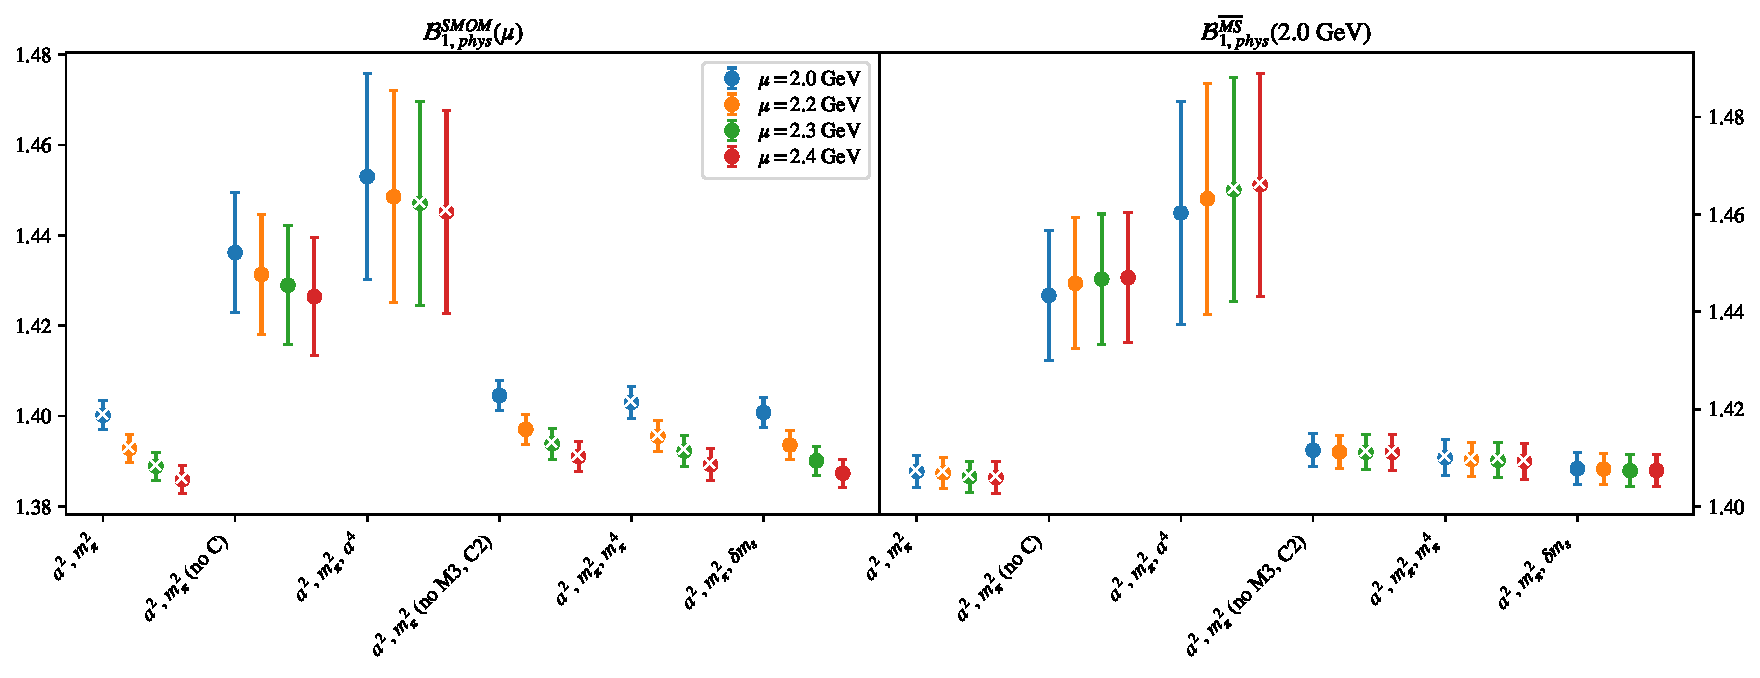
\includegraphics[page=1, width=1.1\textwidth]{VVpAA/NPR/fit_summary_bag.pdf}
\caption{$\mathcal{B}_{1}$\\(left) $\mathcal{B}_{phys}$ in RI/SMOM scheme from fit variations (fits with $p$-value $<0.05$ marked with ``$\times$"). \\(right) $\mathcal{B}_{phys}$ in $\overline{MS}$ computed using $\mathcal{B}^{\overline{MS}} = R^{\overline{MS}\leftarrow SMOM}(2.0)\sigma_{npt}(2.0,\mu) \mathcal{B}^{SMOM}(\mu)$.}
\end{figure}
\clearpage
\begin{figure}
\centering
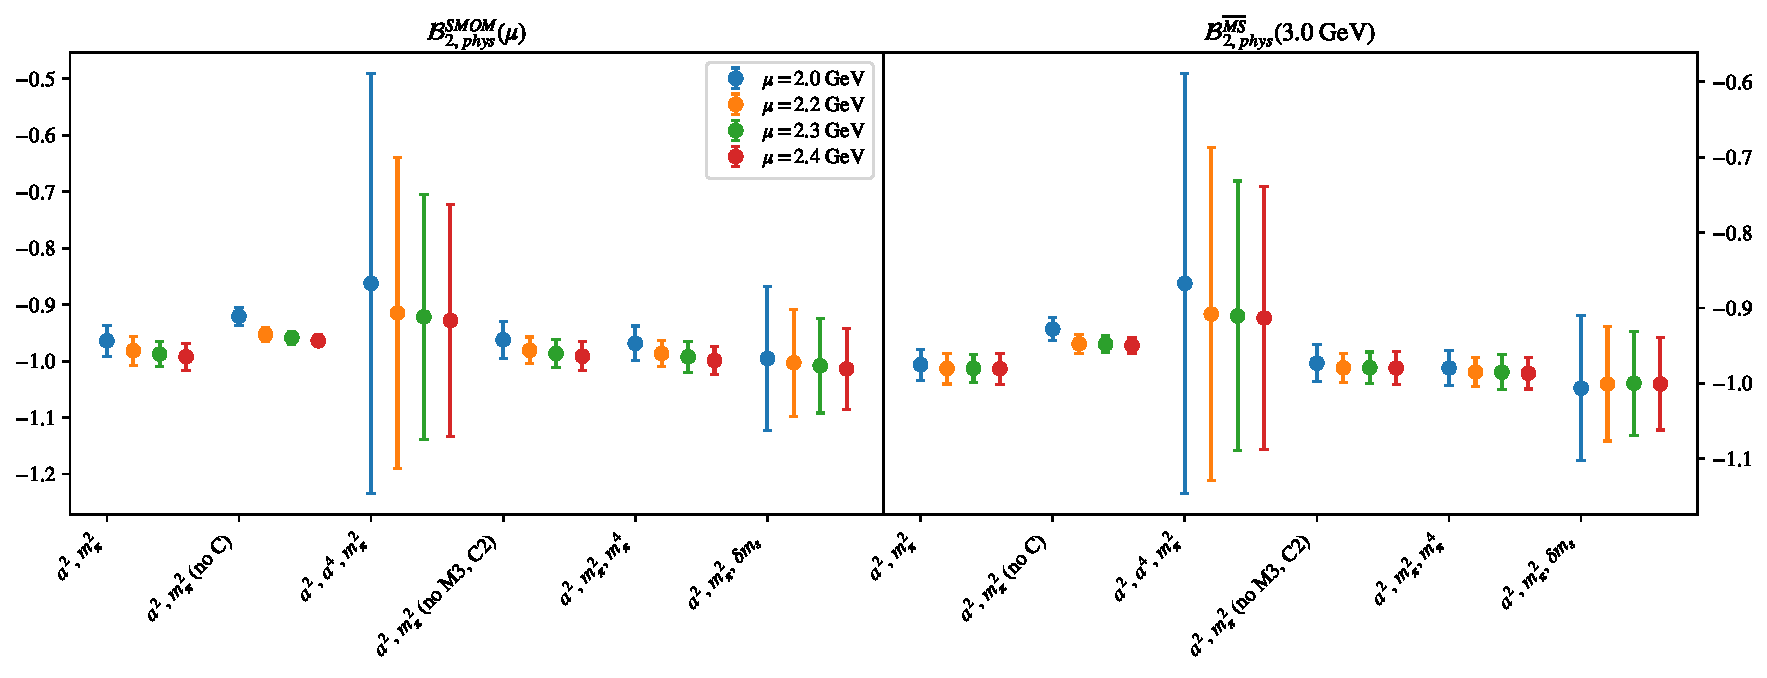
\includegraphics[page=1, width=1.1\textwidth]{VVmAA/NPR/fit_summary_bag.pdf}
\caption{$\mathcal{B}_{2}$\\(left) $\mathcal{B}_{phys}$ in RI/SMOM scheme from fit variations (fits with $p$-value $<0.05$ marked with ``$\times$"). \\(right) $\mathcal{B}_{phys}$ in $\overline{MS}$ computed using $\mathcal{B}^{\overline{MS}} = R^{\overline{MS}\leftarrow SMOM}(3.0)\sigma_{npt}(3.0,\mu) \mathcal{B}^{SMOM}(\mu)$.}
\end{figure}
\clearpage
\begin{figure}
\centering
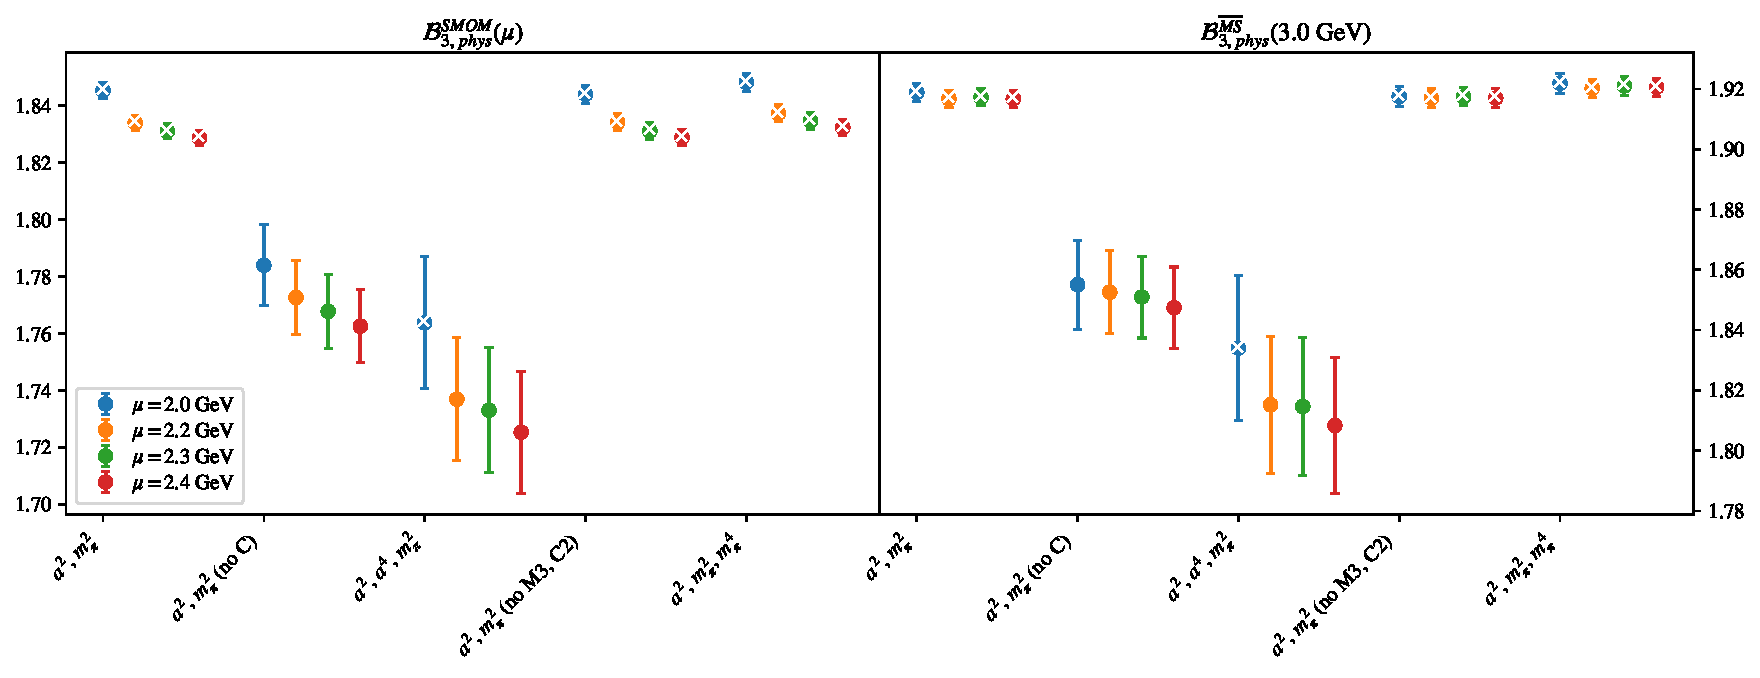
\includegraphics[page=1, width=1.1\textwidth]{SSmPP/NPR/fit_summary_bag.pdf}
\caption{$\mathcal{B}_{3}$\\(left) $\mathcal{B}_{phys}$ in RI/SMOM scheme from fit variations (fits with $p$-value $<0.05$ marked with ``$\times$"). \\(right) $\mathcal{B}_{phys}$ in $\overline{MS}$ computed using $\mathcal{B}^{\overline{MS}} = R^{\overline{MS}\leftarrow SMOM}(3.0)\sigma_{npt}(3.0,\mu) \mathcal{B}^{SMOM}(\mu)$.}
\end{figure}
\clearpage
\begin{figure}
\centering
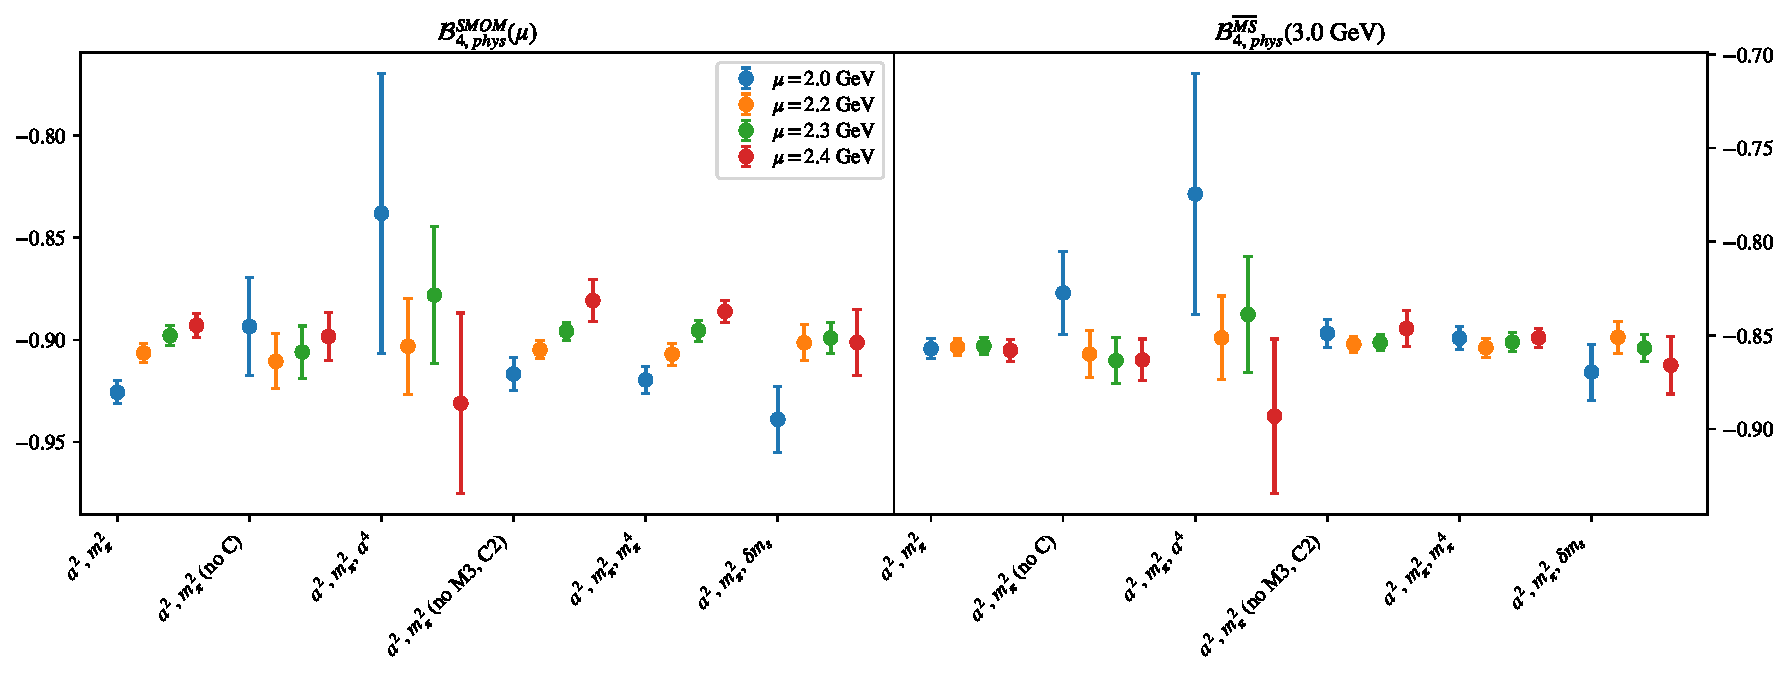
\includegraphics[page=1, width=1.1\textwidth]{SSpPP/NPR/fit_summary_bag.pdf}
\caption{$\mathcal{B}_{4}$\\(left) $\mathcal{B}_{phys}$ in RI/SMOM scheme from fit variations (fits with $p$-value $<0.05$ marked with ``$\times$"). \\(right) $\mathcal{B}_{phys}$ in $\overline{MS}$ computed using $\mathcal{B}^{\overline{MS}} = R^{\overline{MS}\leftarrow SMOM}(3.0)\sigma_{npt}(3.0,\mu) \mathcal{B}^{SMOM}(\mu)$.}
\end{figure}
\clearpage
\begin{figure}
\centering
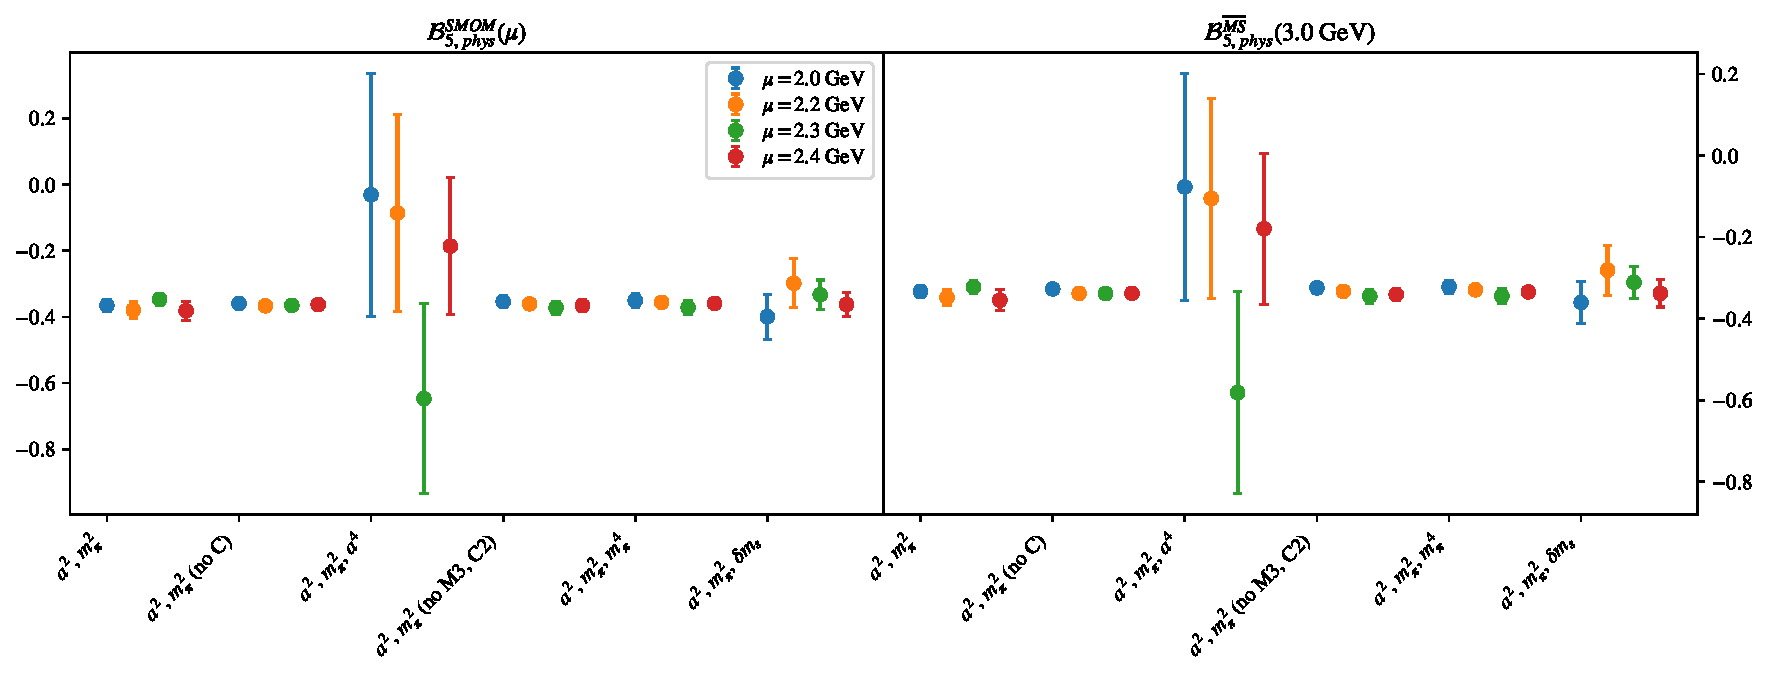
\includegraphics[page=1, width=1.1\textwidth]{TT/NPR/fit_summary_bag.pdf}
\caption{$\mathcal{B}_{5}$\\(left) $\mathcal{B}_{phys}$ in RI/SMOM scheme from fit variations (fits with $p$-value $<0.05$ marked with ``$\times$"). \\(right) $\mathcal{B}_{phys}$ in $\overline{MS}$ computed using $\mathcal{B}^{\overline{MS}} = R^{\overline{MS}\leftarrow SMOM}(3.0)\sigma_{npt}(3.0,\mu) \mathcal{B}^{SMOM}(\mu)$.}
\end{figure}
\clearpage
\section{$\mathcal{B}_1$}
\begin{table}[h!]
\begin{center}
\begin{tabular}{|c|c|c|c|c|c|c|}
\hline
$\mu$ (GeV) & $a^2$, $m_\pi^2$& $a^2$, $m_\pi^2$ (no C)& $a^2$, $m_\pi^2$, $a^4$& $a^2$, $m_\pi^2$ (no M3, C2)& $a^2$, $m_\pi^2$, $m_\pi^4$& $a^2$, $m_\pi^2$, $\delta m_s$\\
\hline
2.0& \hyperlink{VVpAA/NPR/bag_a2m2_20.pdf.1}{\textbf{1.4019(28)}: 2.288 (0.043)} & \hyperlink{VVpAA/NPR/bag_a2m2noC_20.pdf.1}{\textbf{1.436(12)}: 0.226 (0.797)} & \hyperlink{VVpAA/NPR/bag_a2a4m2_20.pdf.1}{\textbf{1.455(22)}: 1.374 (0.24)} & \hyperlink{VVpAA/NPR/bag_a2m2mcut_20.pdf.1}{\textbf{1.4055(32)}: 1.926 (0.123)} & \hyperlink{VVpAA/NPR/bag_a2m2m4_20.pdf.1}{\textbf{1.4046(34)}: 2.309 (0.055)} & \hyperlink{VVpAA/NPR/bag_a2m2delm_20.pdf.1}{\textbf{1.4027(30)}: 0.771 (0.544)}\\
2.2& \hyperlink{VVpAA/NPR/bag_a2m2_22.pdf.1}{\textbf{1.3942(28)}: 2.785 (0.016)} & \hyperlink{VVpAA/NPR/bag_a2m2noC_22.pdf.1}{\textbf{1.431(12)}: 0.357 (0.7)} & \hyperlink{VVpAA/NPR/bag_a2a4m2_22.pdf.1}{\textbf{1.452(22)}: 1.782 (0.129)} & \hyperlink{VVpAA/NPR/bag_a2m2mcut_22.pdf.1}{\textbf{1.3983(32)}: 2.262 (0.079)} & \hyperlink{VVpAA/NPR/bag_a2m2m4_22.pdf.1}{\textbf{1.3971(33)}: 2.61 (0.034)} & \hyperlink{VVpAA/NPR/bag_a2m2delm_22.pdf.1}{\textbf{1.3951(29)}: 0.976 (0.419)}\\
2.3& \hyperlink{VVpAA/NPR/bag_a2m2_23.pdf.1}{\textbf{1.3906(28)}: 2.823 (0.015)} & \hyperlink{VVpAA/NPR/bag_a2m2noC_23.pdf.1}{\textbf{1.428(12)}: 0.354 (0.702)} & \hyperlink{VVpAA/NPR/bag_a2a4m2_23.pdf.1}{\textbf{1.449(22)}: 1.774 (0.131)} & \hyperlink{VVpAA/NPR/bag_a2m2mcut_23.pdf.1}{\textbf{1.3950(31)}: 2.367 (0.069)} & \hyperlink{VVpAA/NPR/bag_a2m2m4_23.pdf.1}{\textbf{1.3939(33)}: 2.751 (0.027)} & \hyperlink{VVpAA/NPR/bag_a2m2delm_23.pdf.1}{\textbf{1.3919(29)}: 0.995 (0.409)}\\
2.4& \hyperlink{VVpAA/NPR/bag_a2m2_24.pdf.1}{\textbf{1.3879(28)}: 2.926 (0.012)} & \hyperlink{VVpAA/NPR/bag_a2m2noC_24.pdf.1}{\textbf{1.425(12)}: 0.387 (0.679)} & \hyperlink{VVpAA/NPR/bag_a2a4m2_24.pdf.1}{\textbf{1.447(22)}: 1.879 (0.111)} & \hyperlink{VVpAA/NPR/bag_a2m2mcut_24.pdf.1}{\textbf{1.3923(31)}: 2.395 (0.066)} & \hyperlink{VVpAA/NPR/bag_a2m2m4_24.pdf.1}{\textbf{1.3910(33)}: 2.746 (0.027)} & \hyperlink{VVpAA/NPR/bag_a2m2delm_24.pdf.1}{\textbf{1.3891(29)}: 1.03 (0.39)}\\
\hline
\end{tabular}
\caption{Physical point value from chiral and continuum extrapolation at renormalisation scale $\mu$. Entries are \textbf{value(error)}: $\chi^2/\text{DOF}$ ($p$-value).}
\end{center}
\end{table}
\begin{table}[h!]
\begin{center}
\begin{tabular}{|c c|c|c|c|c|c|c|}
\hline
$\mu$ (GeV) &  & $a^2$, $m_\pi^2$& $a^2$, $m_\pi^2$ (no C)& $a^2$, $m_\pi^2$, $a^4$& $a^2$, $m_\pi^2$ (no M3, C2)& $a^2$, $m_\pi^2$, $m_\pi^4$& $a^2$, $m_\pi^2$, $\delta m_s$\\
\hline
\multirow{3}{0.5in}{2.0} & $\alpha$ & 0.140(10)& -0.054(76)& -0.35(20)& 0.129(11)& 0.132(11)& 0.141(10)\\
 & $\beta$ & 0.00374(20)& 0.00335(38)& 0.00402(23)& 0.00316(32)& 0.0021(10)& 0.00501(50)\\
 & $\gamma$ &  &  & 1.00(42)&  & 0.000147(92)& -0.050(18)\\
\hline
\multirow{3}{0.5in}{2.2} & $\alpha$ & 0.146(10)& -0.062(76)& -0.38(20)& 0.133(11)& 0.137(11)& 0.147(10)\\
 & $\beta$ & 0.00372(20)& 0.00329(39)& 0.00401(23)& 0.00307(33)& 0.0019(10)& 0.00508(51)\\
 & $\gamma$ &  &  & 1.08(41)&  & 0.000162(91)& -0.053(18)\\
\hline
\multirow{3}{0.5in}{2.3} & $\alpha$ & 0.148(10)& -0.064(76)& -0.38(20)& 0.135(11)& 0.139(11)& 0.149(10)\\
 & $\beta$ & 0.00373(20)& 0.00327(39)& 0.00402(23)& 0.00306(32)& 0.0019(10)& 0.00511(50)\\
 & $\gamma$ &  &  & 1.08(41)&  & 0.000165(92)& -0.054(18)\\
\hline
\multirow{3}{0.5in}{2.4} & $\alpha$ & 0.149(10)& -0.064(76)& -0.39(20)& 0.135(11)& 0.140(11)& 0.150(10)\\
 & $\beta$ & 0.00373(20)& 0.00327(38)& 0.00404(22)& 0.00306(32)& 0.0019(10)& 0.00513(50)\\
 & $\gamma$ &  &  & 1.10(41)&  & 0.000167(90)& -0.054(18)\\
\hline
\end{tabular}
\caption{Fit values of coefficients in $Q = Q_{phys} + \mathbf{\alpha} a^2 + \mathbf{\beta}\left(\frac{m_\pi^2}{f_\pi^2}-\frac{m_{\pi,PDG}^2}{f_\pi^2}\right) + \gamma(\ldots)$}
\end{center}
\end{table}
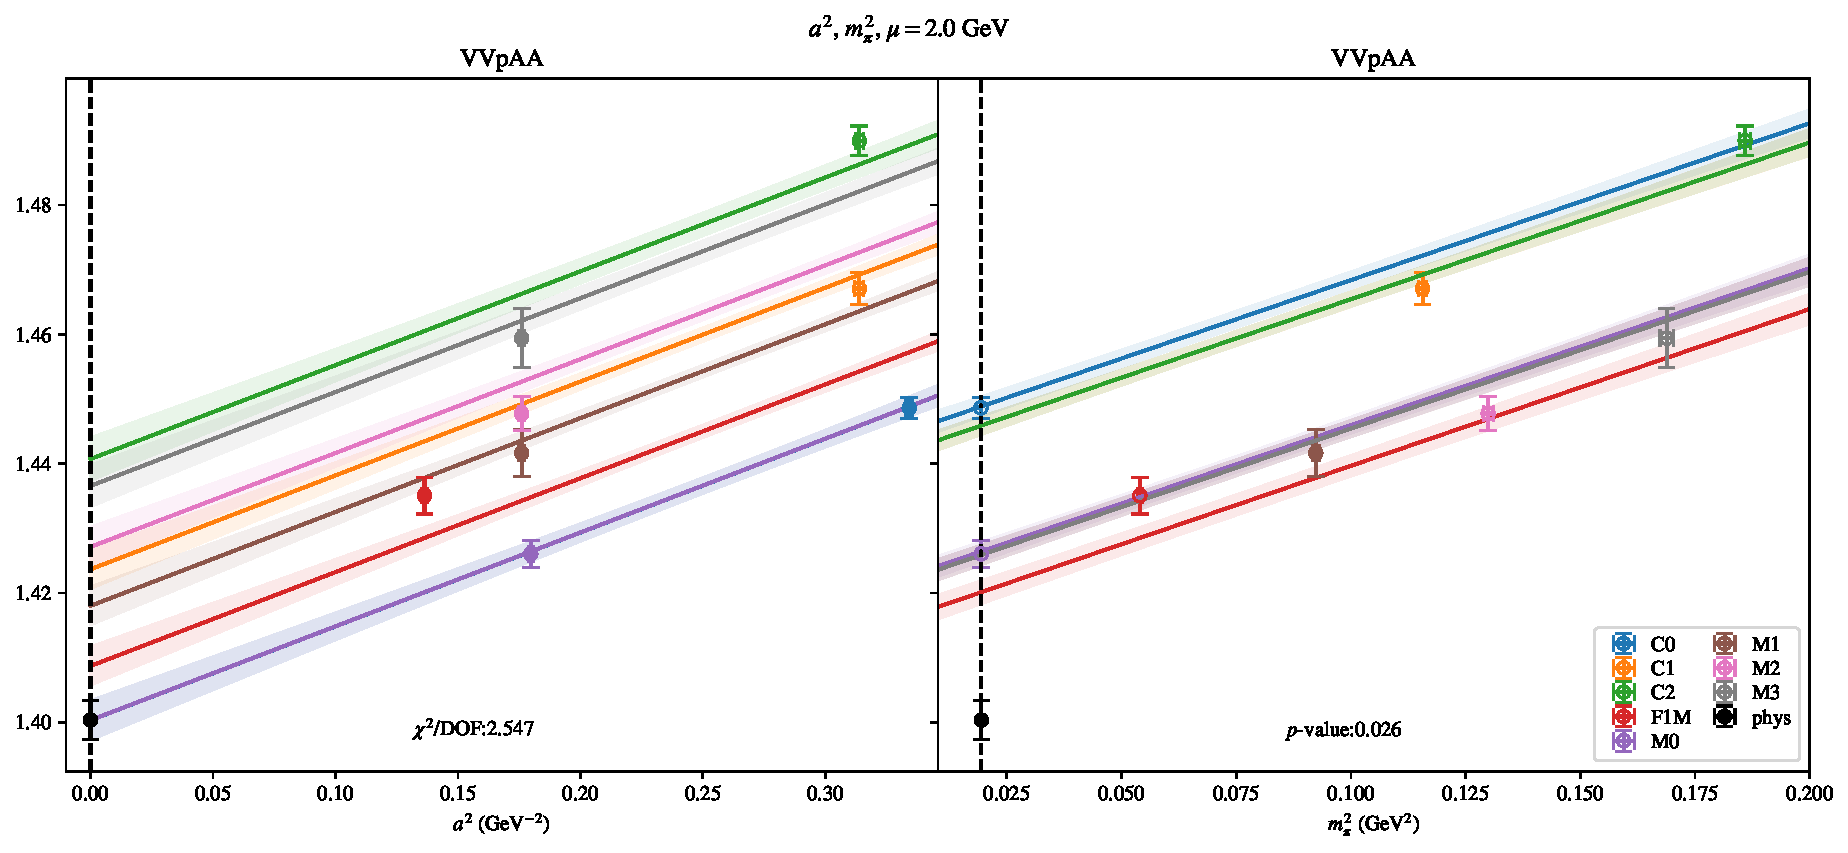
\includepdf[link, pages=-]{VVpAA/NPR/bag_a2m2_20.pdf}
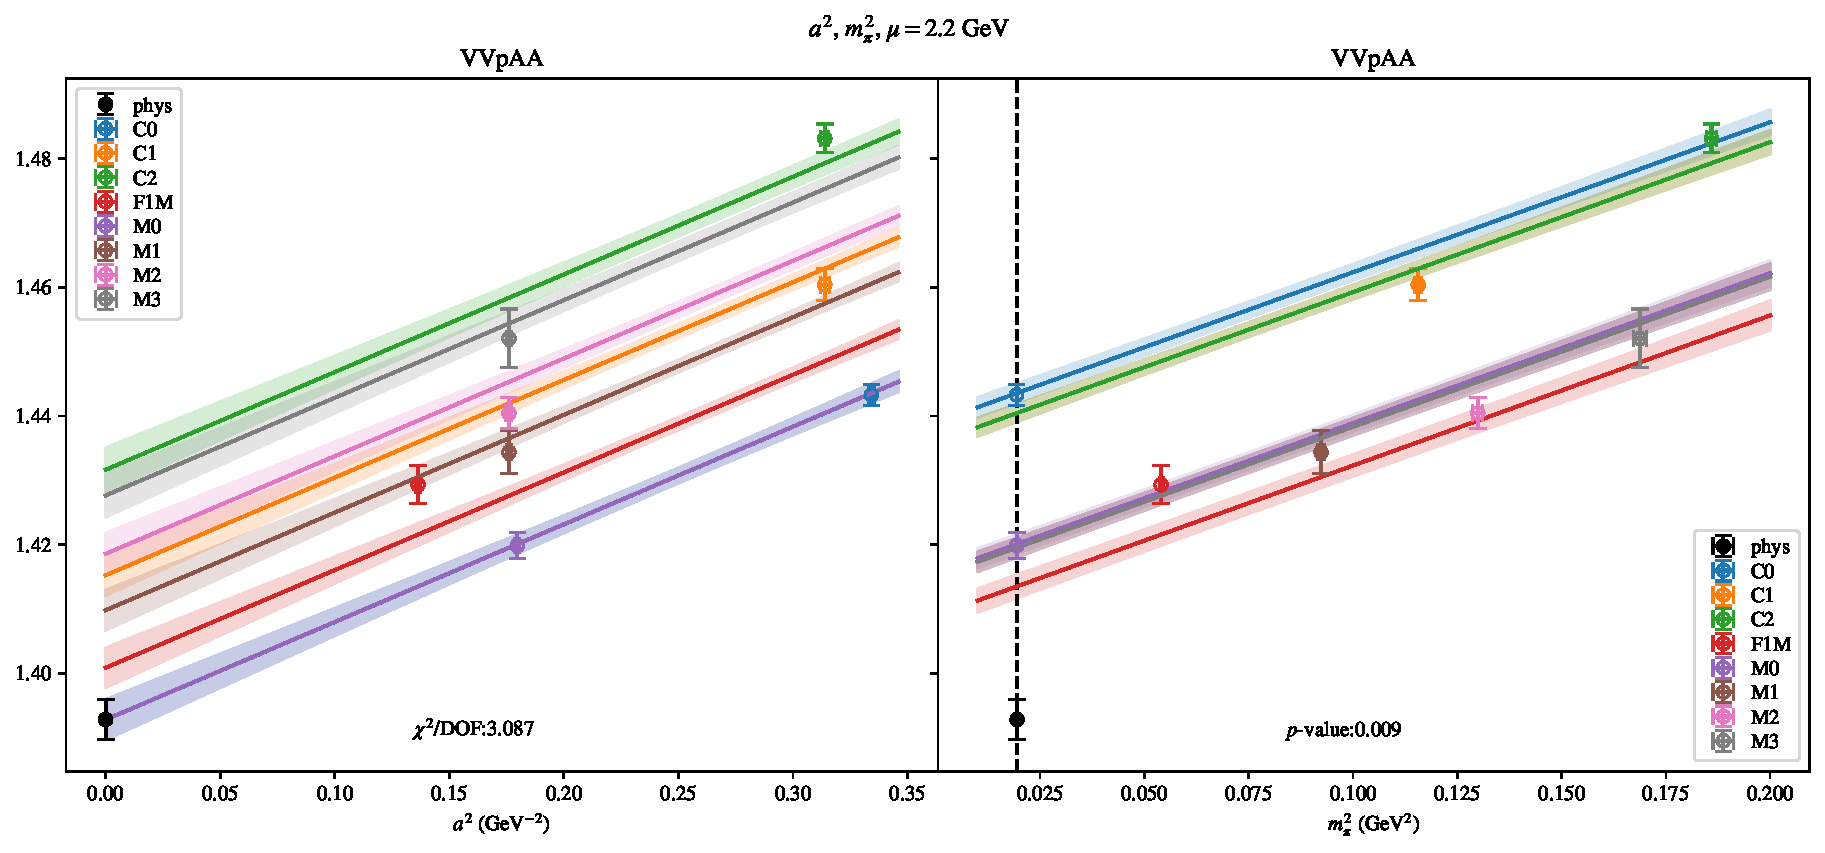
\includepdf[link, pages=-]{VVpAA/NPR/bag_a2m2_22.pdf}
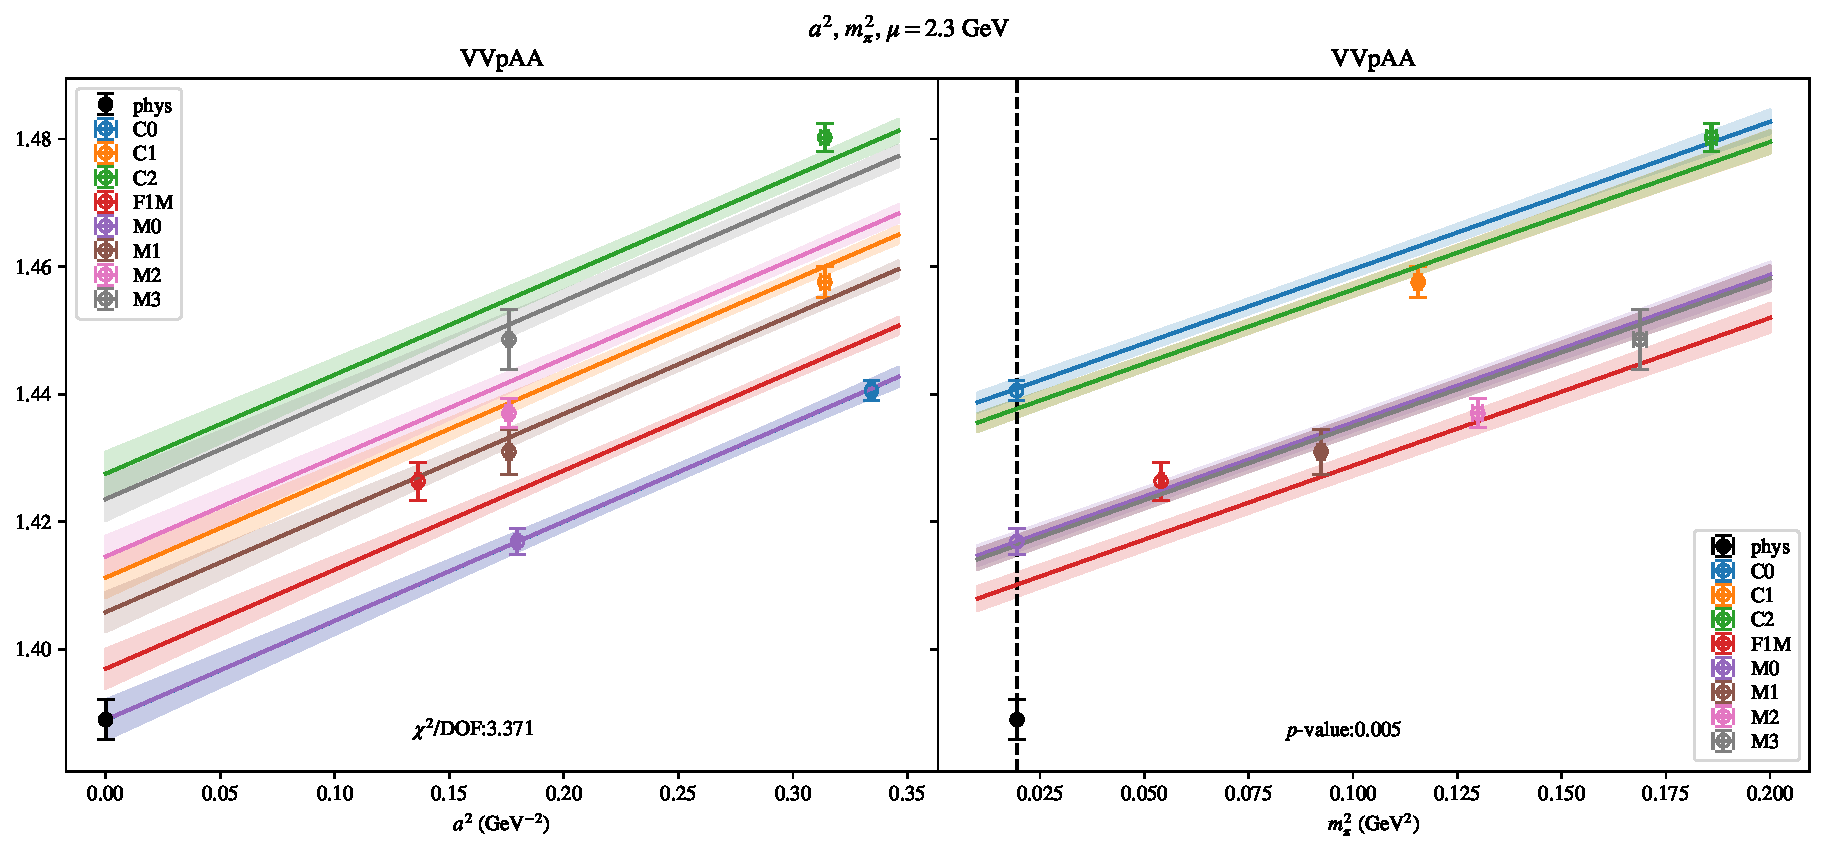
\includepdf[link, pages=-]{VVpAA/NPR/bag_a2m2_23.pdf}
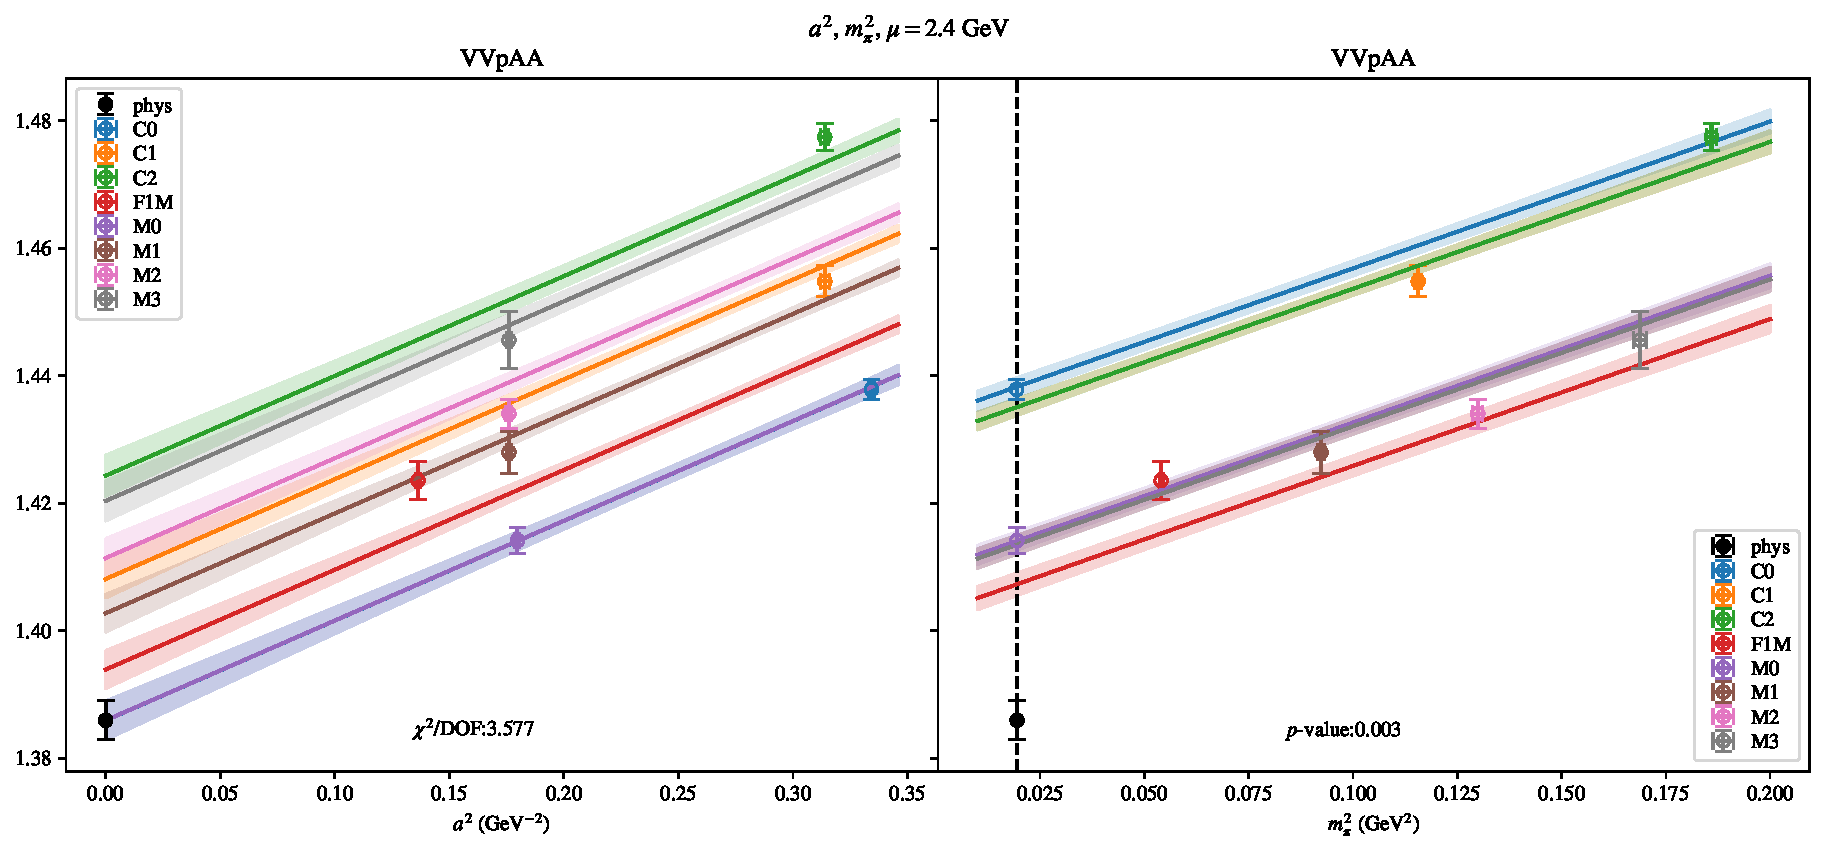
\includepdf[link, pages=-]{VVpAA/NPR/bag_a2m2_24.pdf}
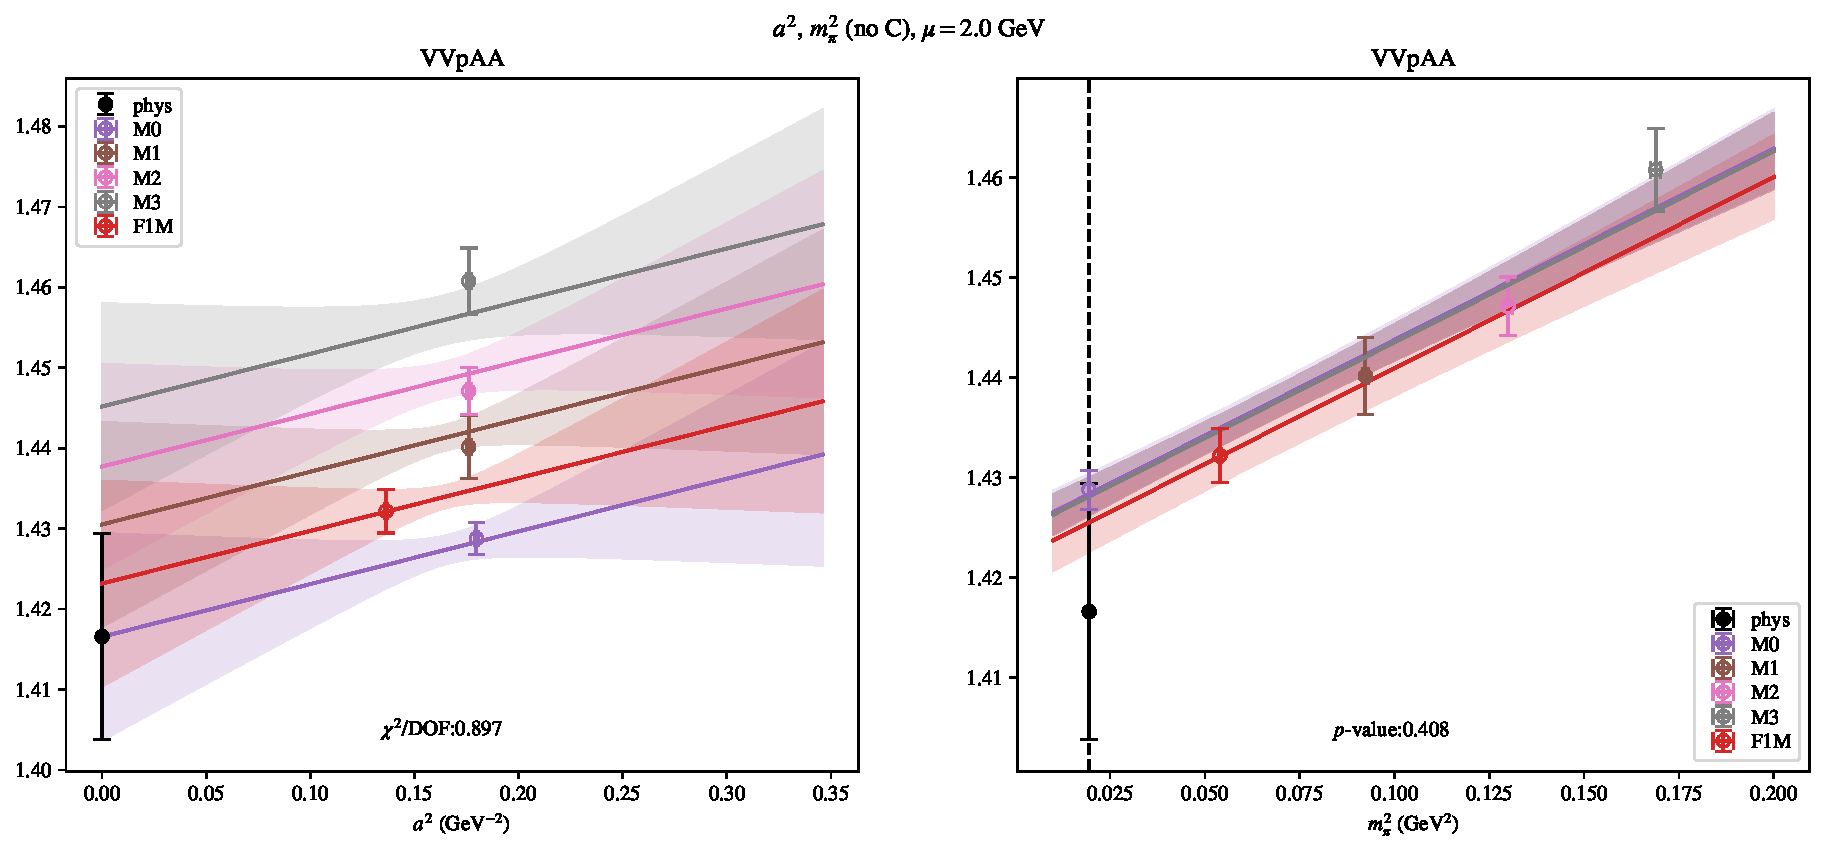
\includepdf[link, pages=-]{VVpAA/NPR/bag_a2m2noC_20.pdf}
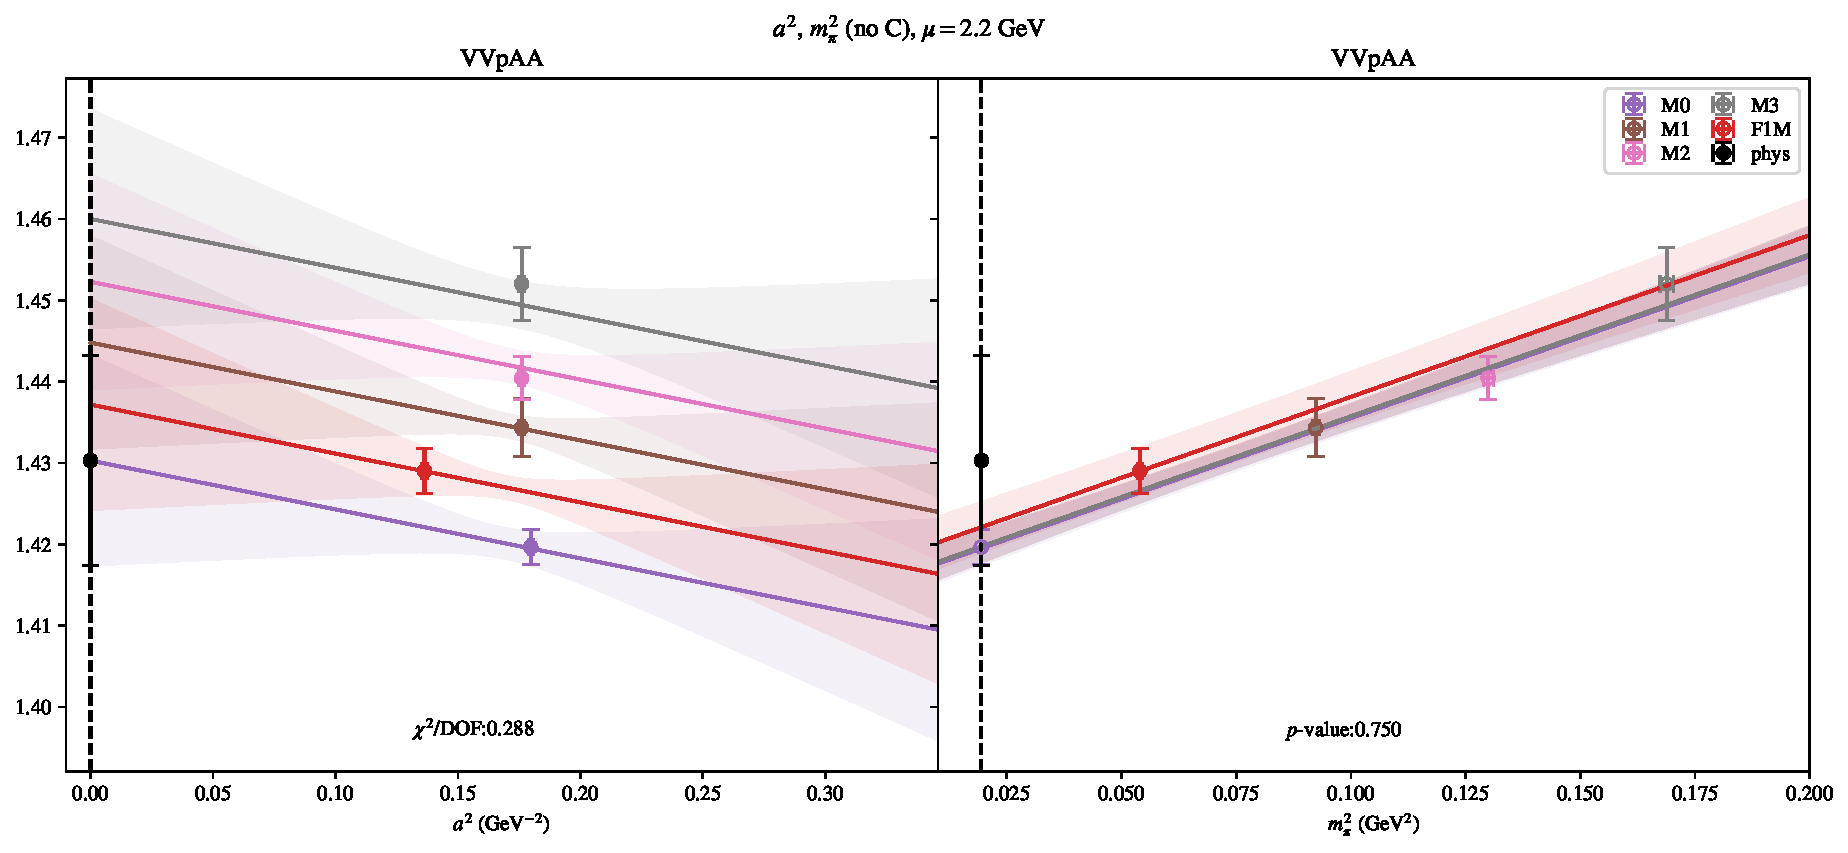
\includepdf[link, pages=-]{VVpAA/NPR/bag_a2m2noC_22.pdf}
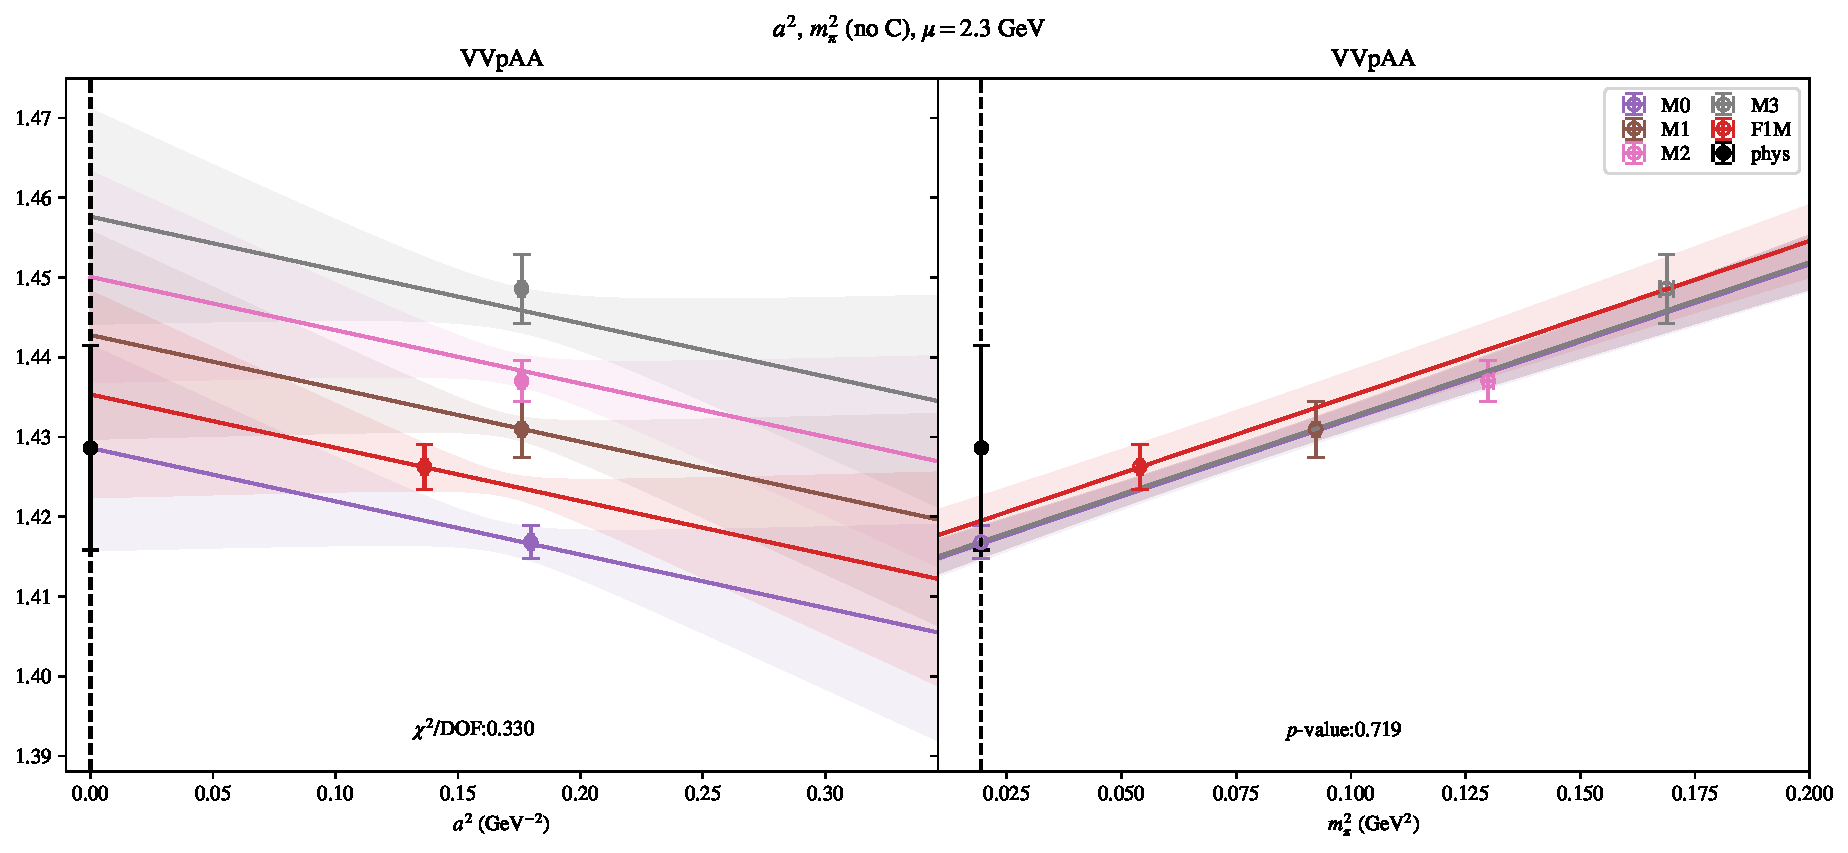
\includepdf[link, pages=-]{VVpAA/NPR/bag_a2m2noC_23.pdf}
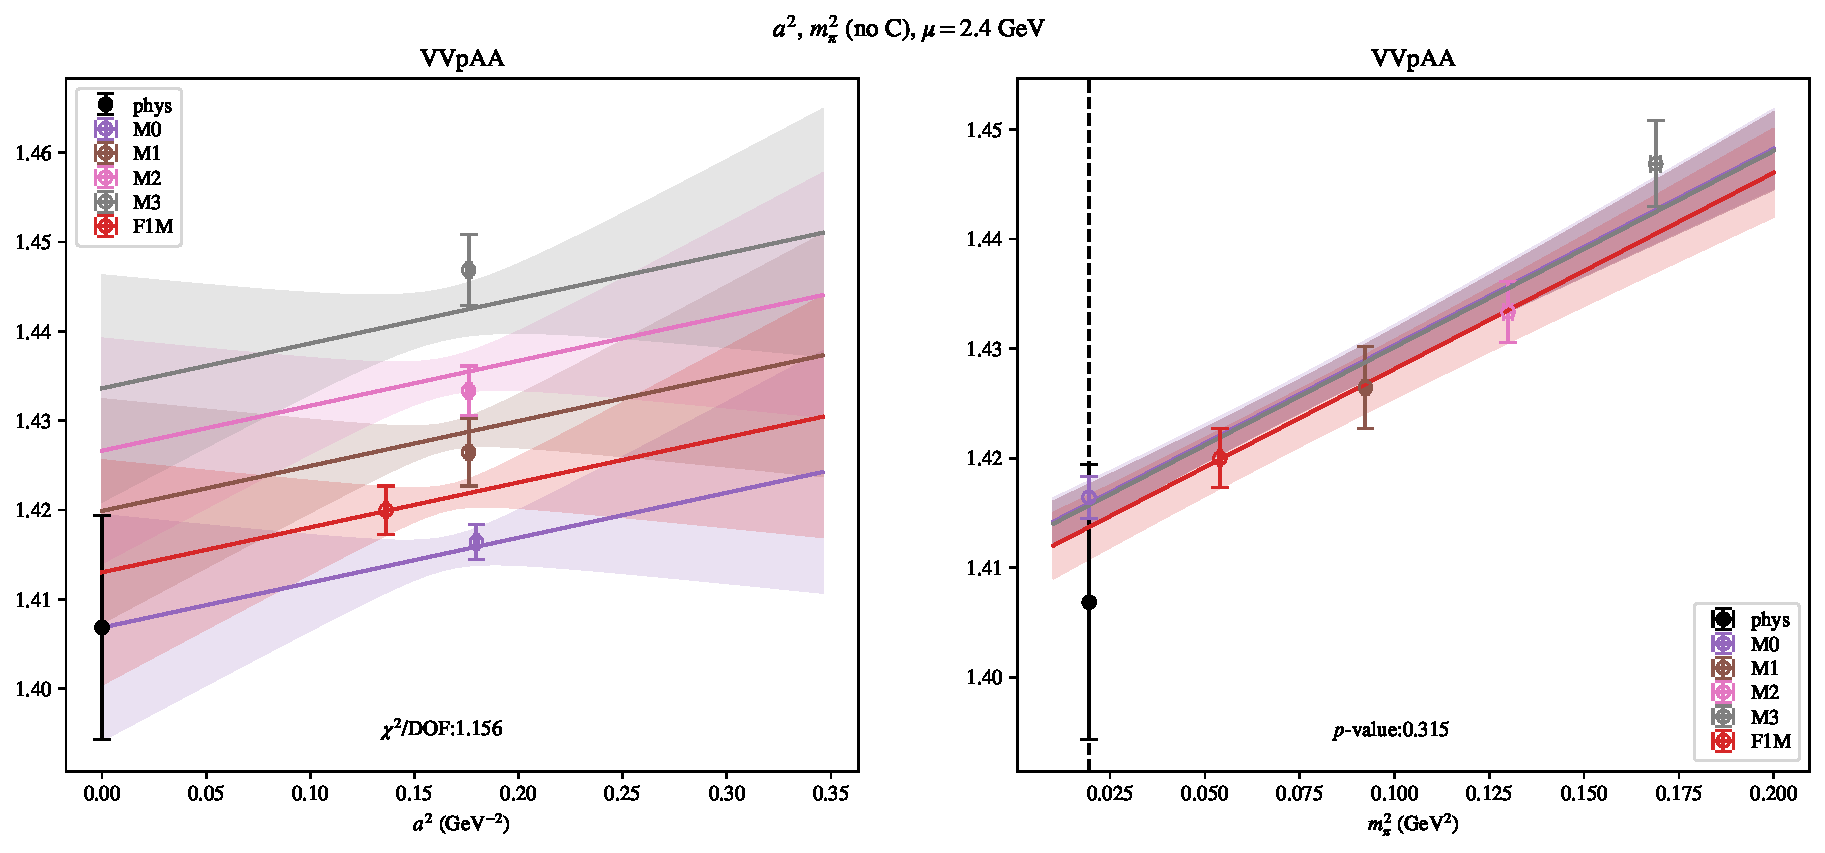
\includepdf[link, pages=-]{VVpAA/NPR/bag_a2m2noC_24.pdf}
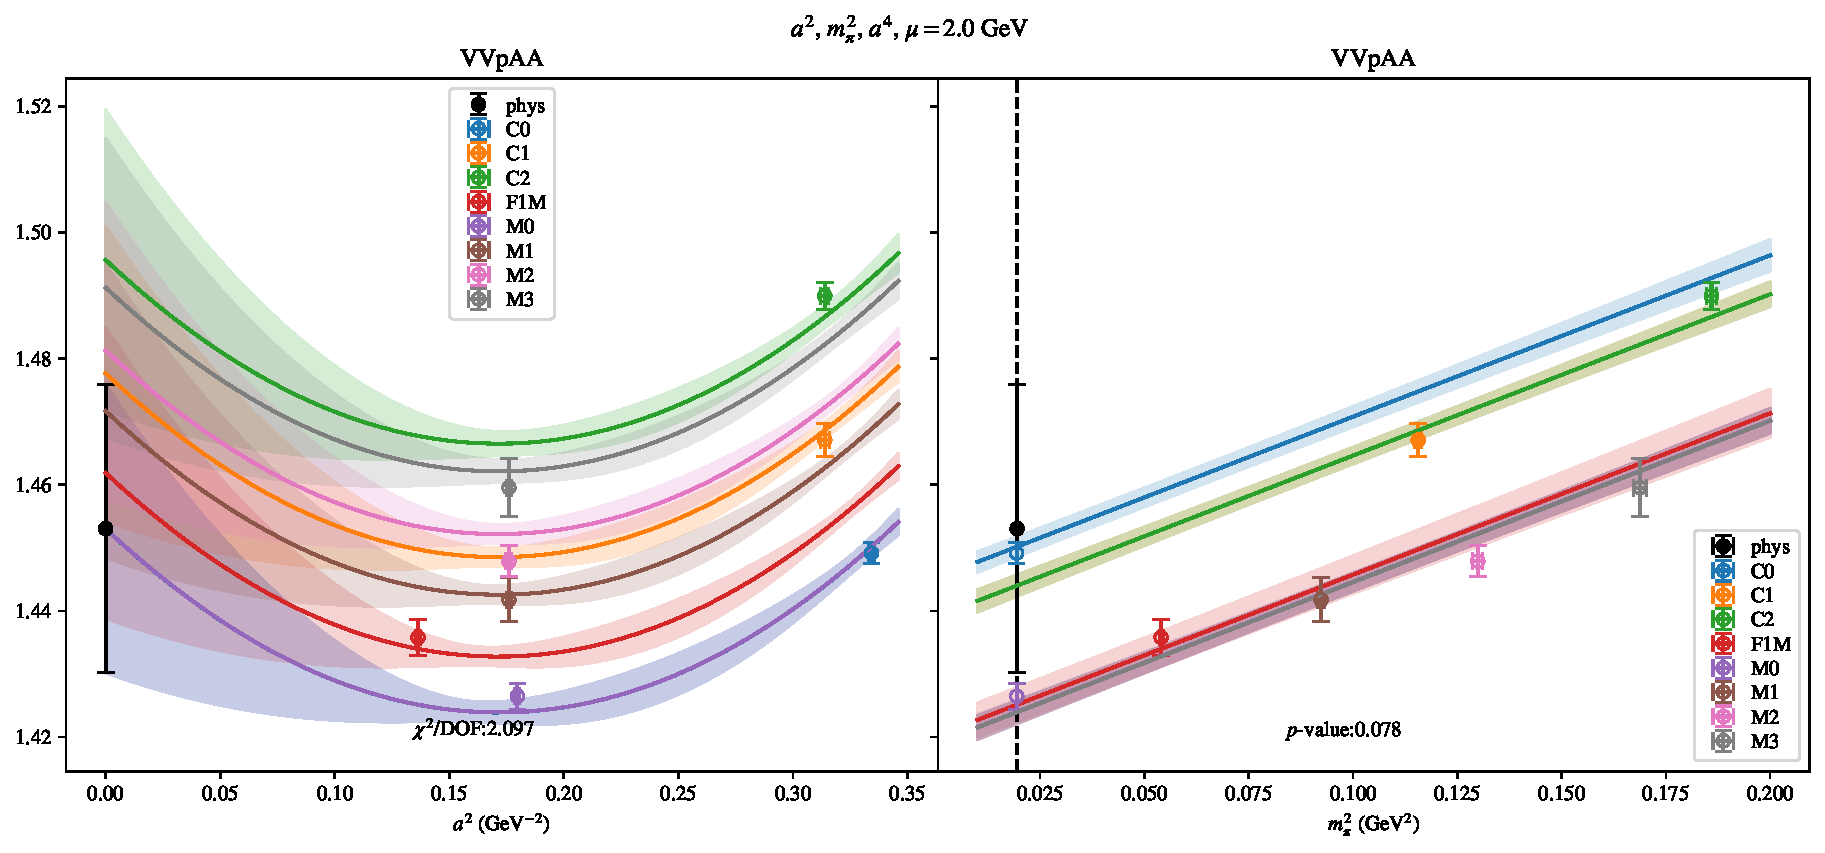
\includepdf[link, pages=-]{VVpAA/NPR/bag_a2a4m2_20.pdf}
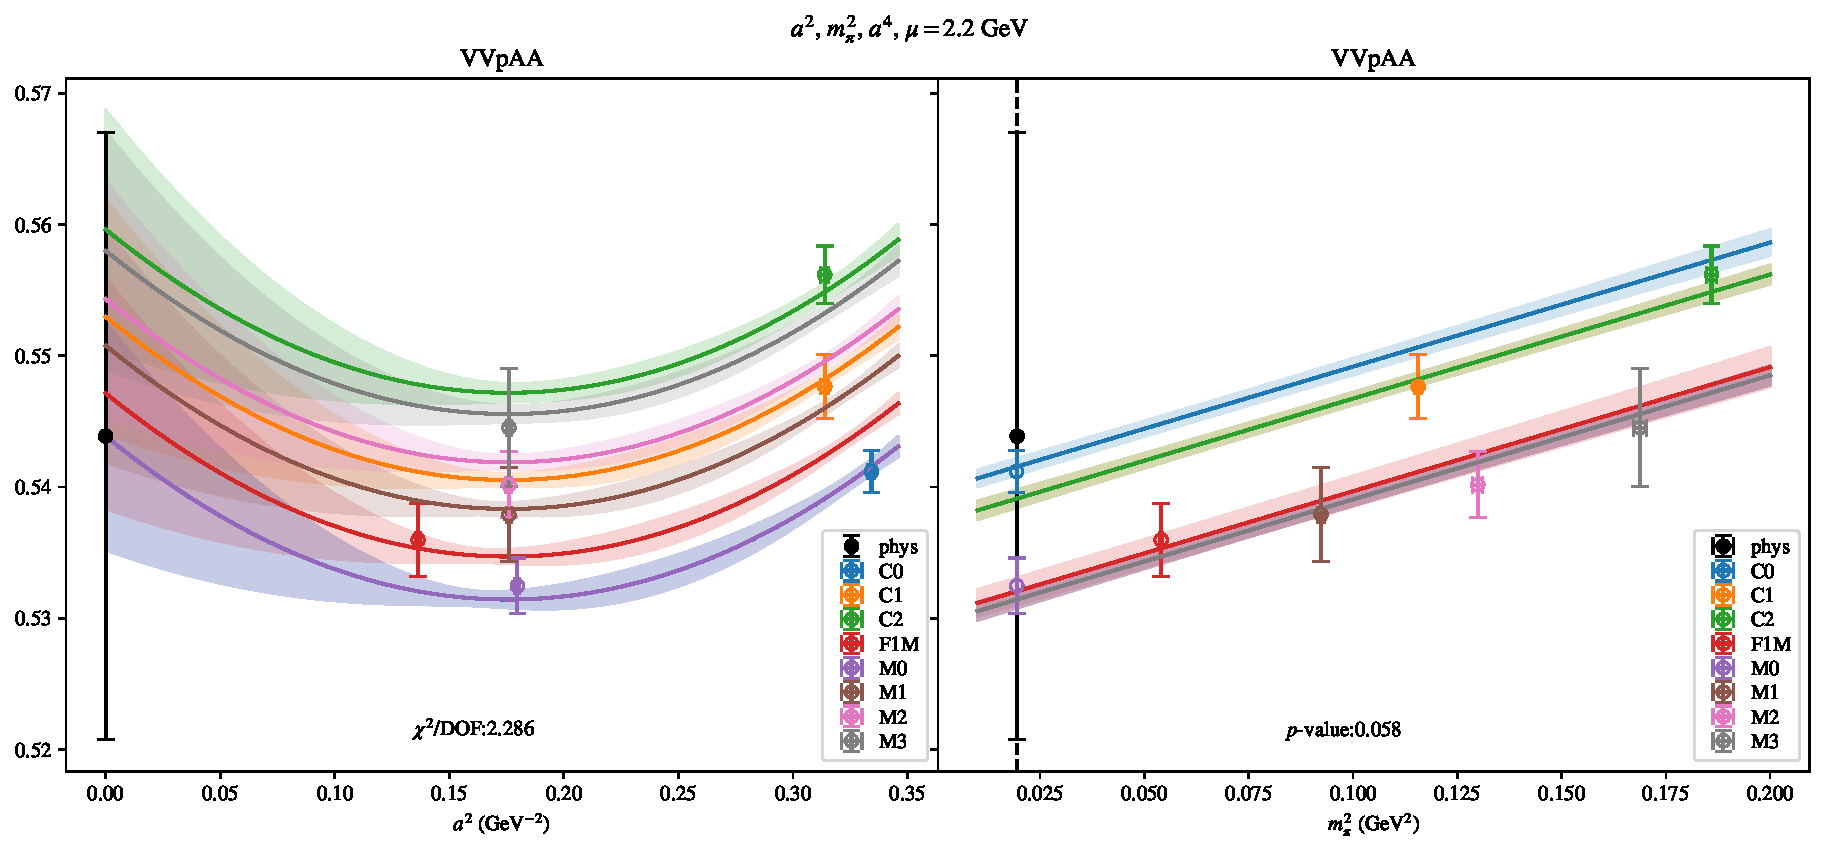
\includepdf[link, pages=-]{VVpAA/NPR/bag_a2a4m2_22.pdf}
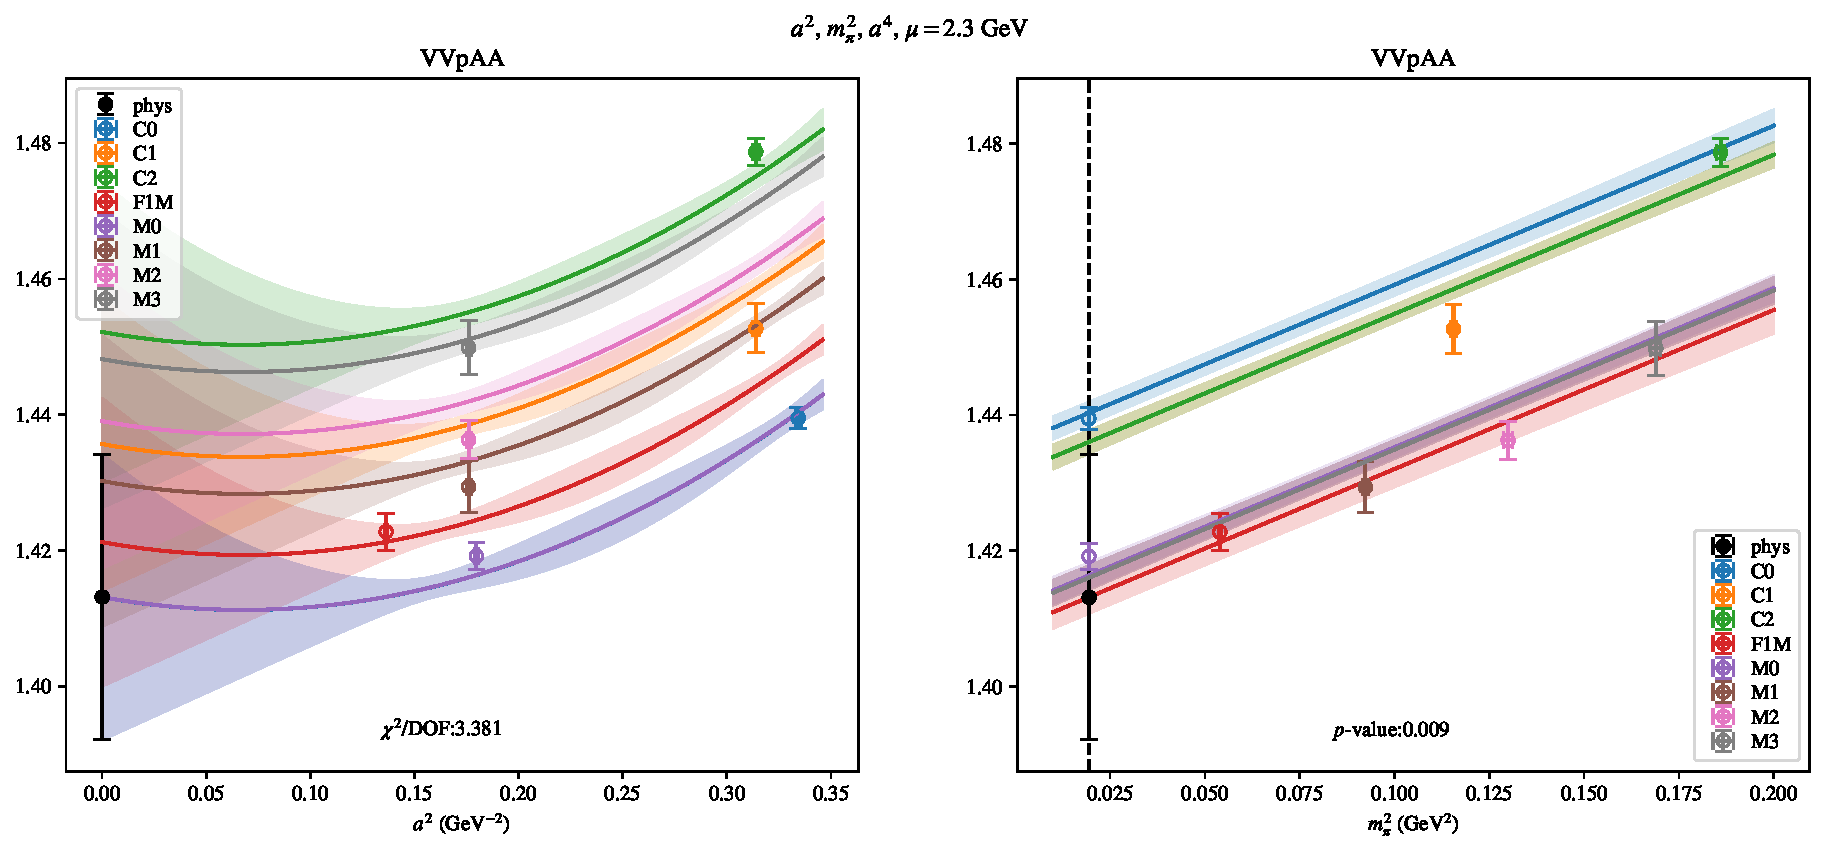
\includepdf[link, pages=-]{VVpAA/NPR/bag_a2a4m2_23.pdf}
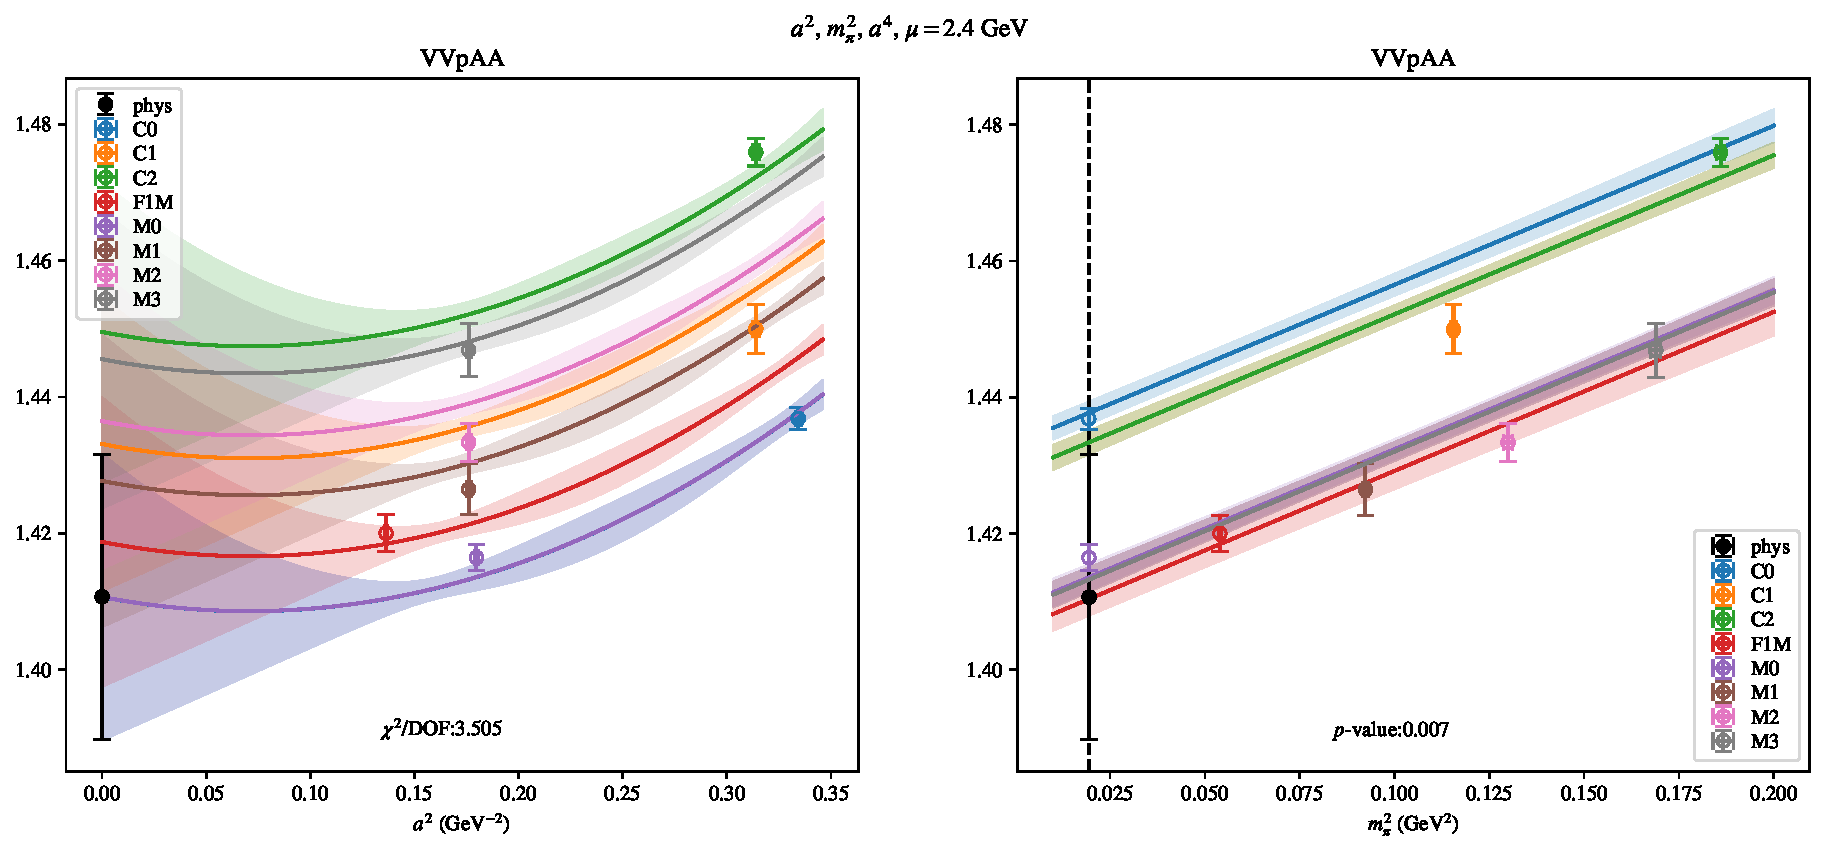
\includepdf[link, pages=-]{VVpAA/NPR/bag_a2a4m2_24.pdf}
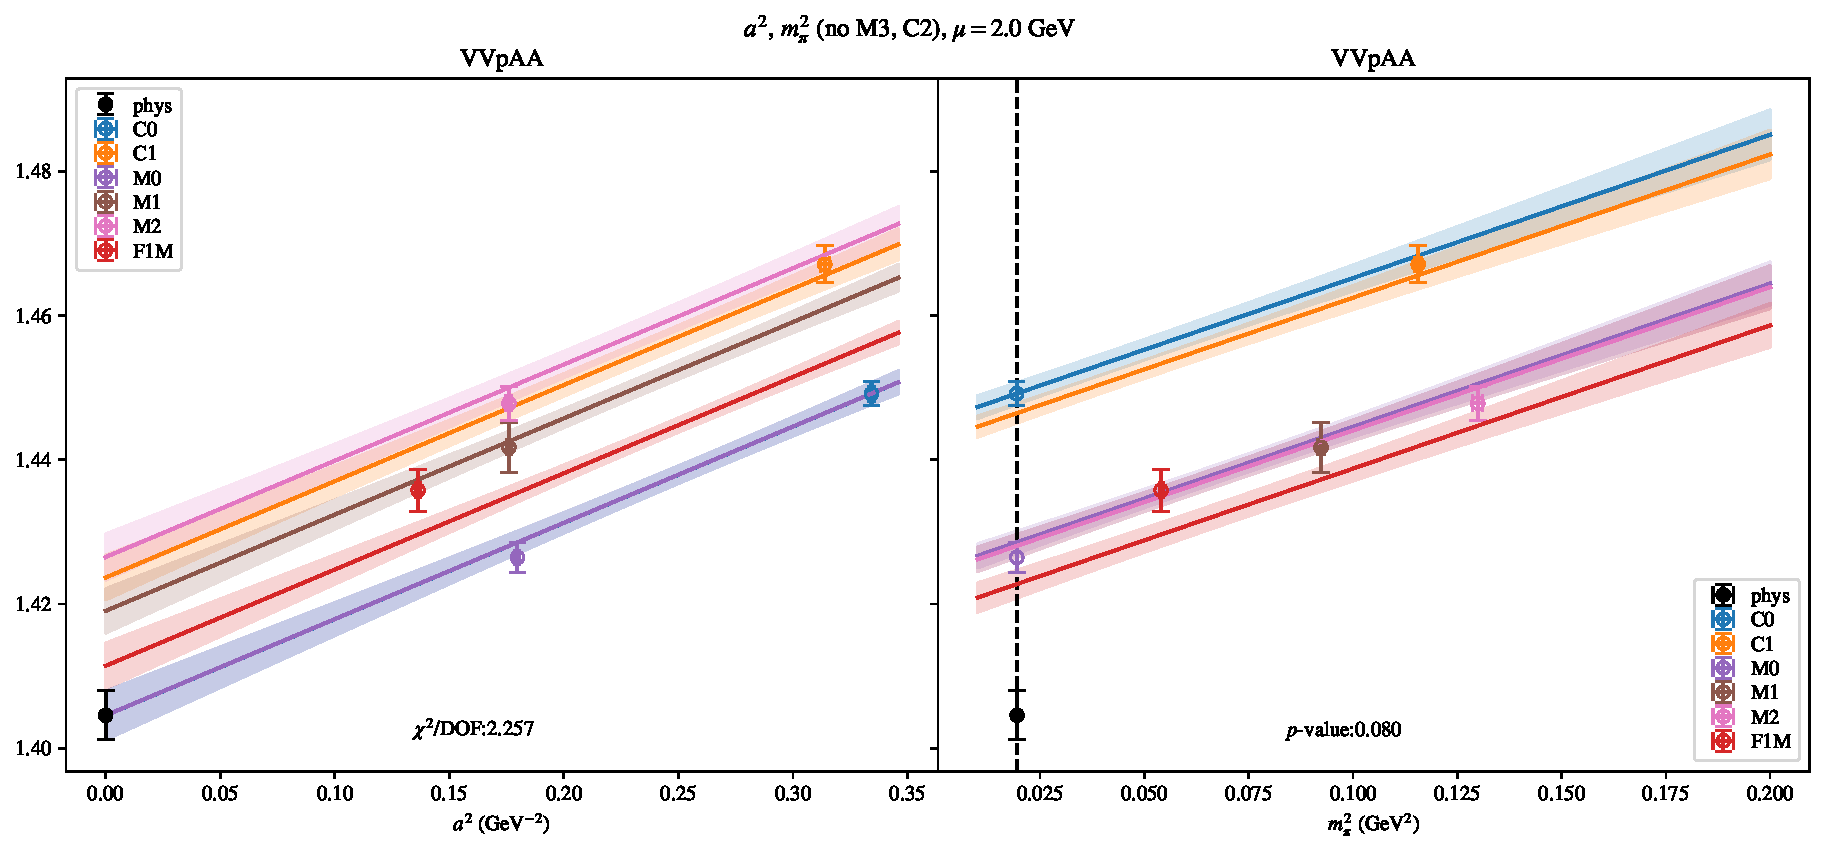
\includepdf[link, pages=-]{VVpAA/NPR/bag_a2m2mcut_20.pdf}
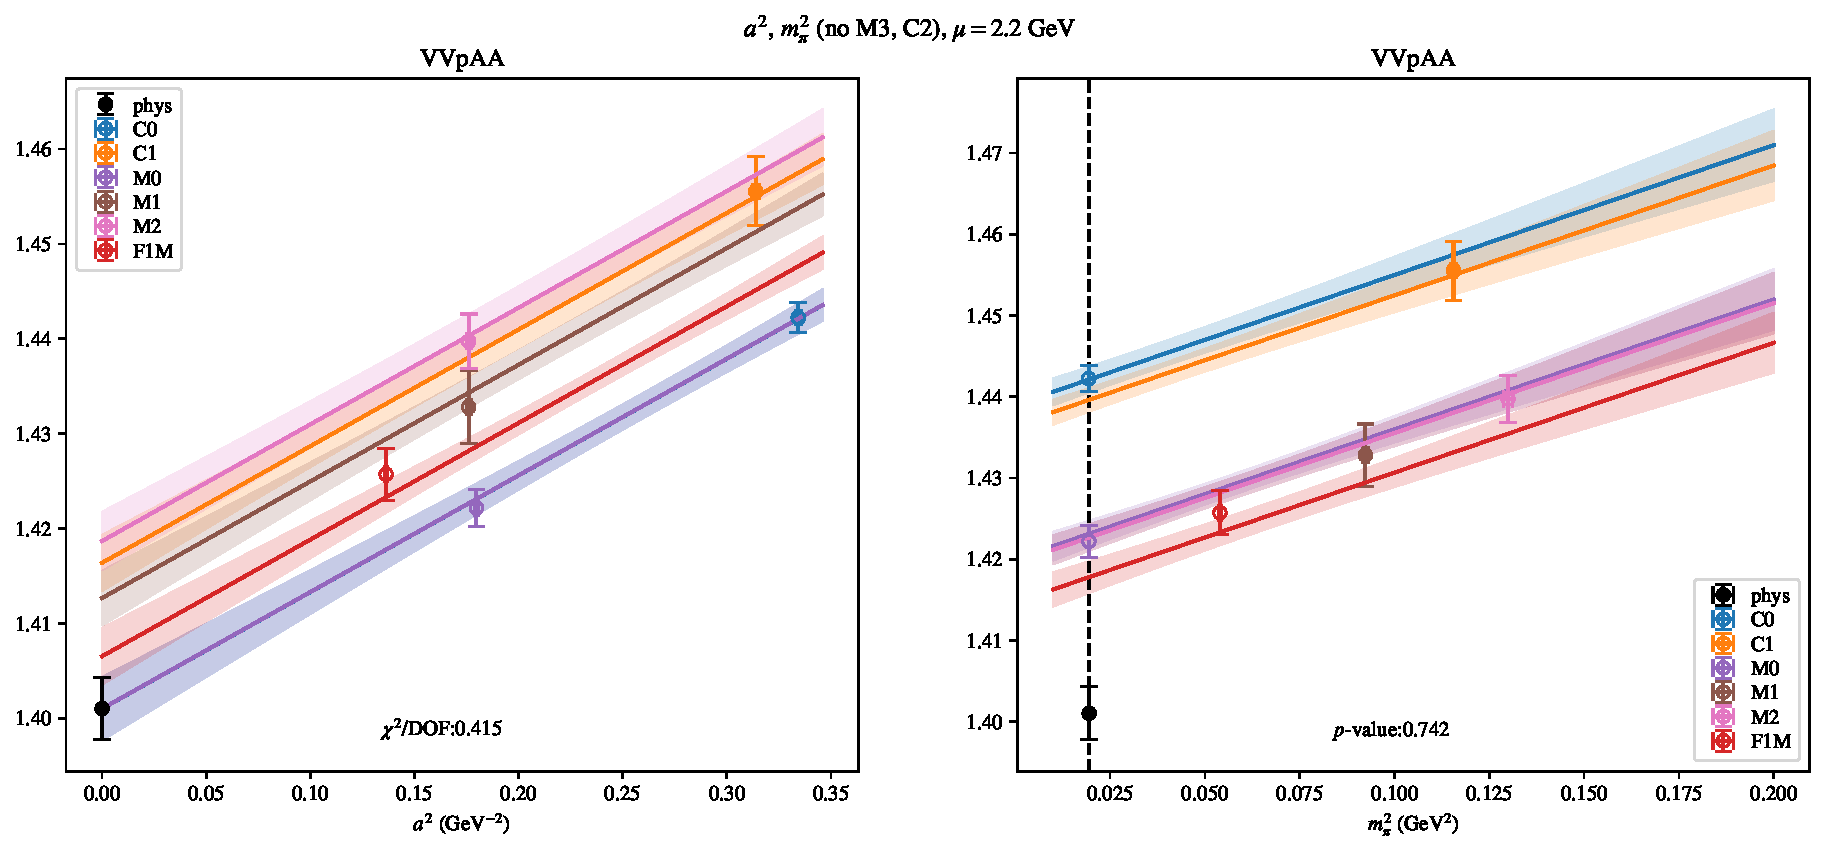
\includepdf[link, pages=-]{VVpAA/NPR/bag_a2m2mcut_22.pdf}
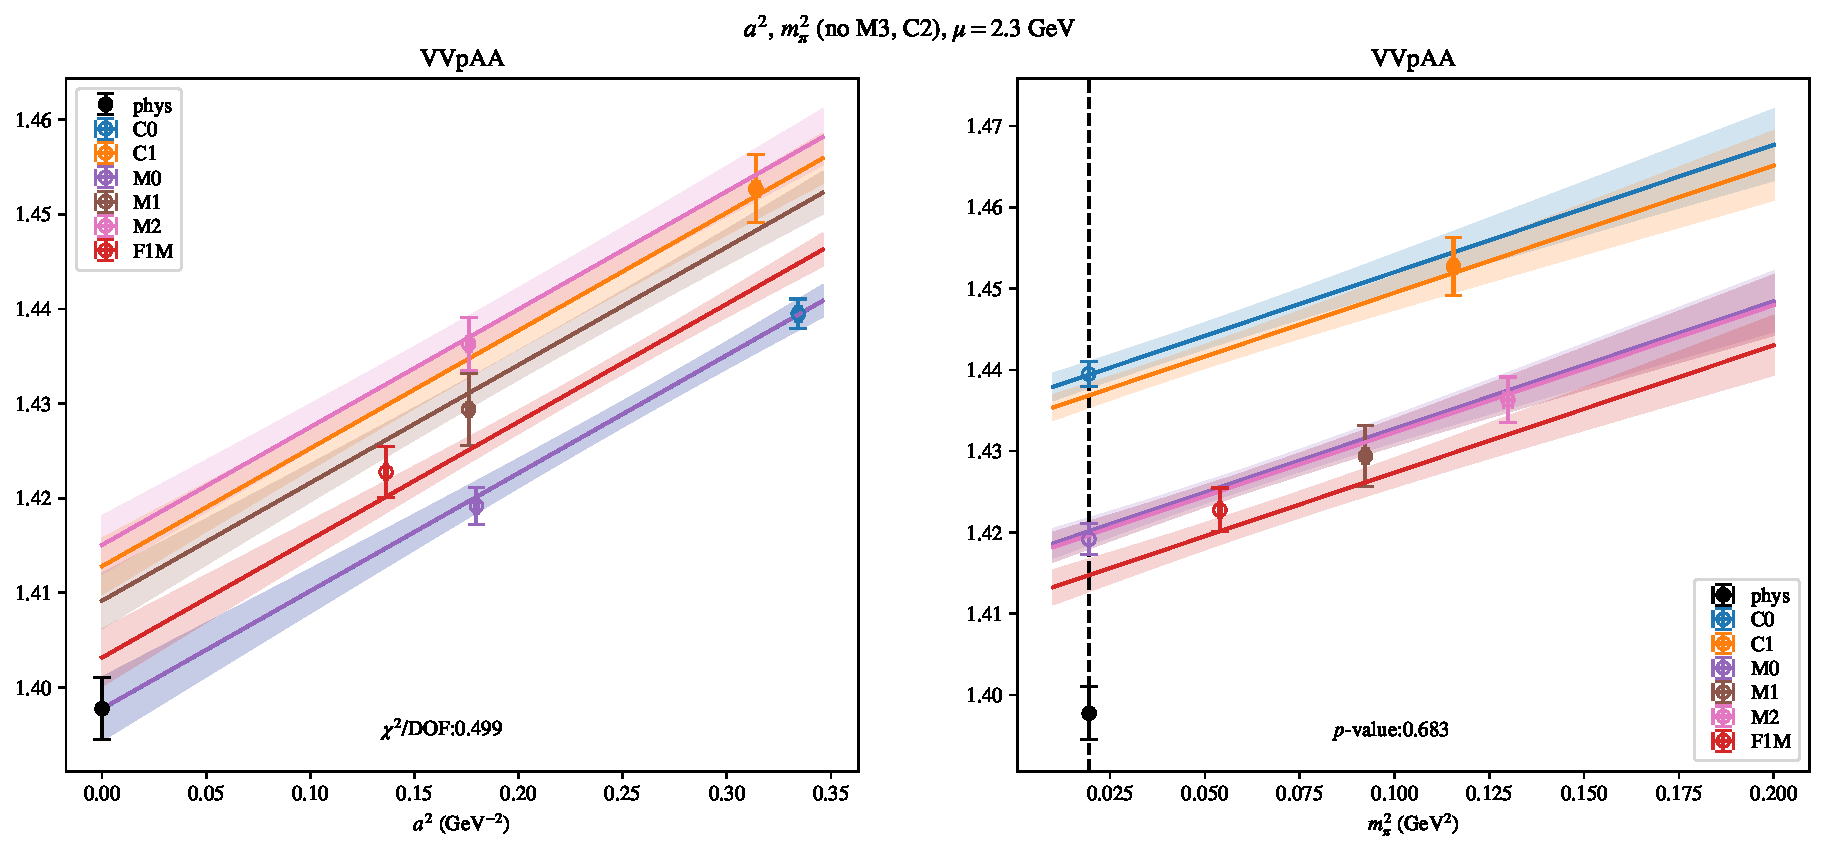
\includepdf[link, pages=-]{VVpAA/NPR/bag_a2m2mcut_23.pdf}
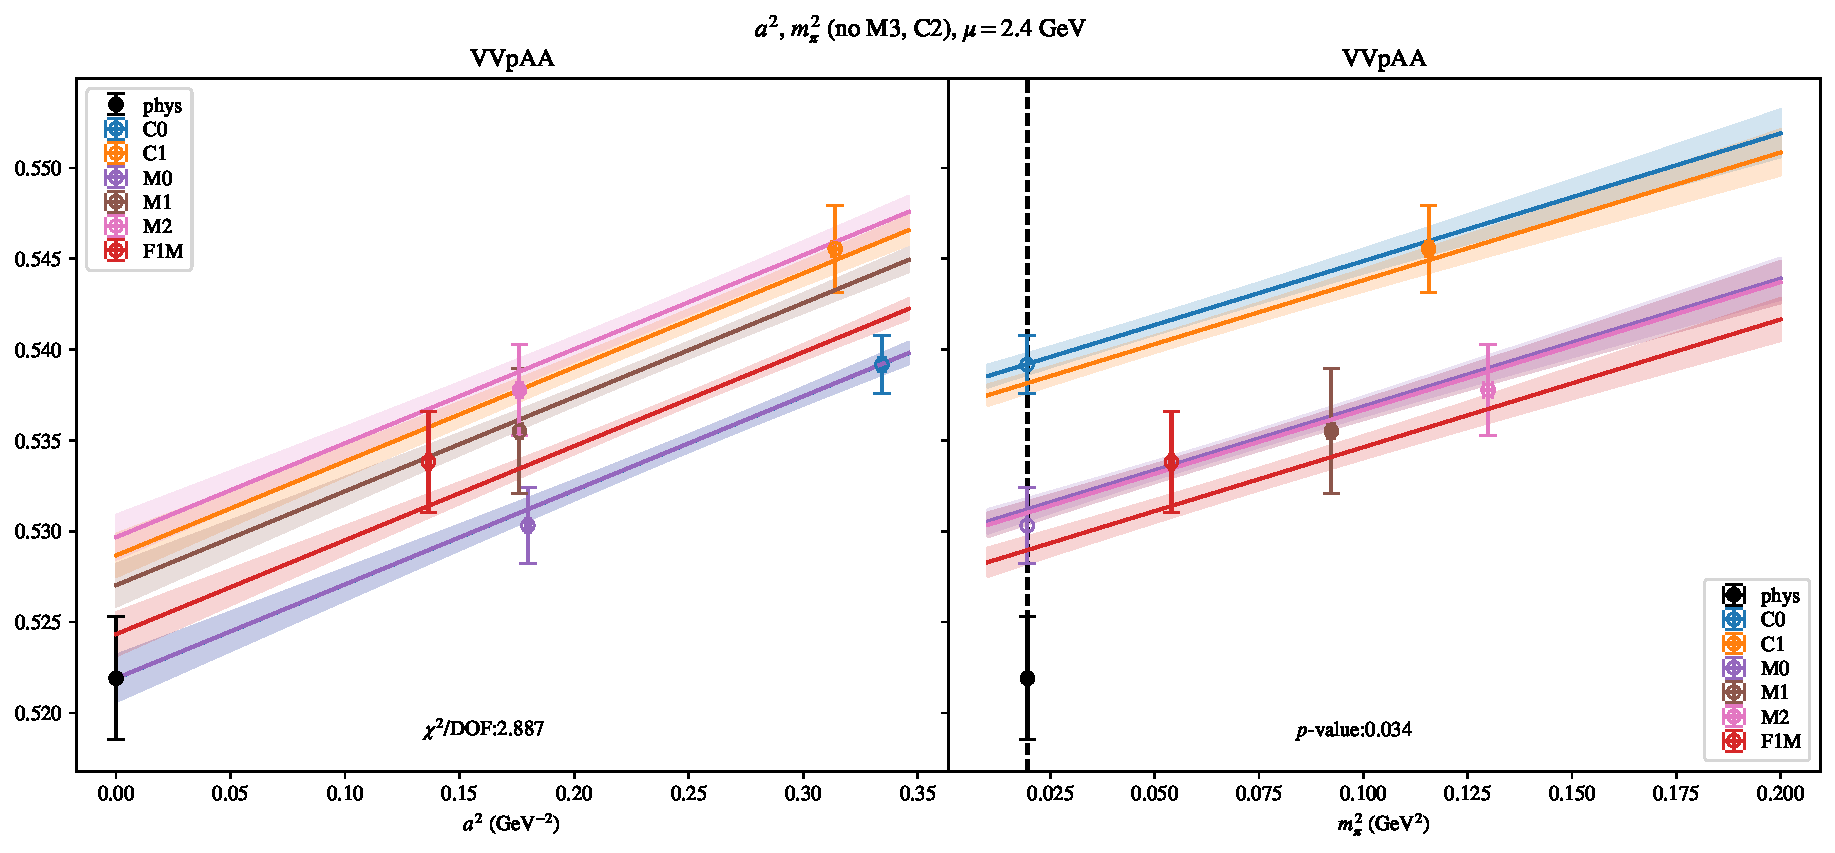
\includepdf[link, pages=-]{VVpAA/NPR/bag_a2m2mcut_24.pdf}
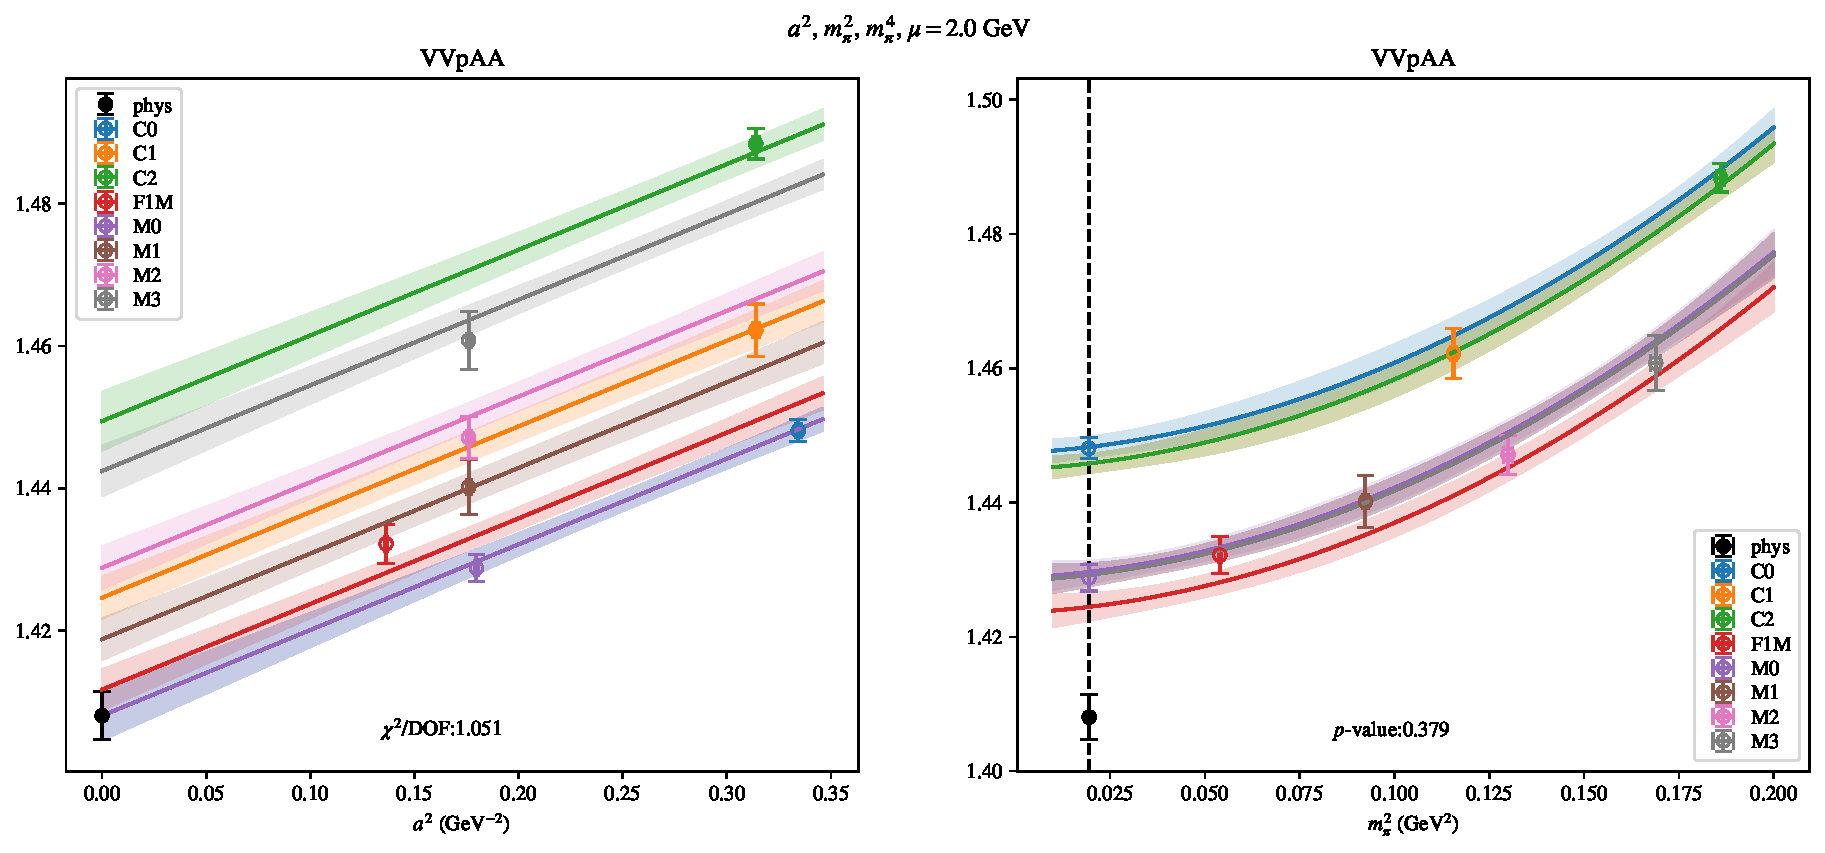
\includepdf[link, pages=-]{VVpAA/NPR/bag_a2m2m4_20.pdf}
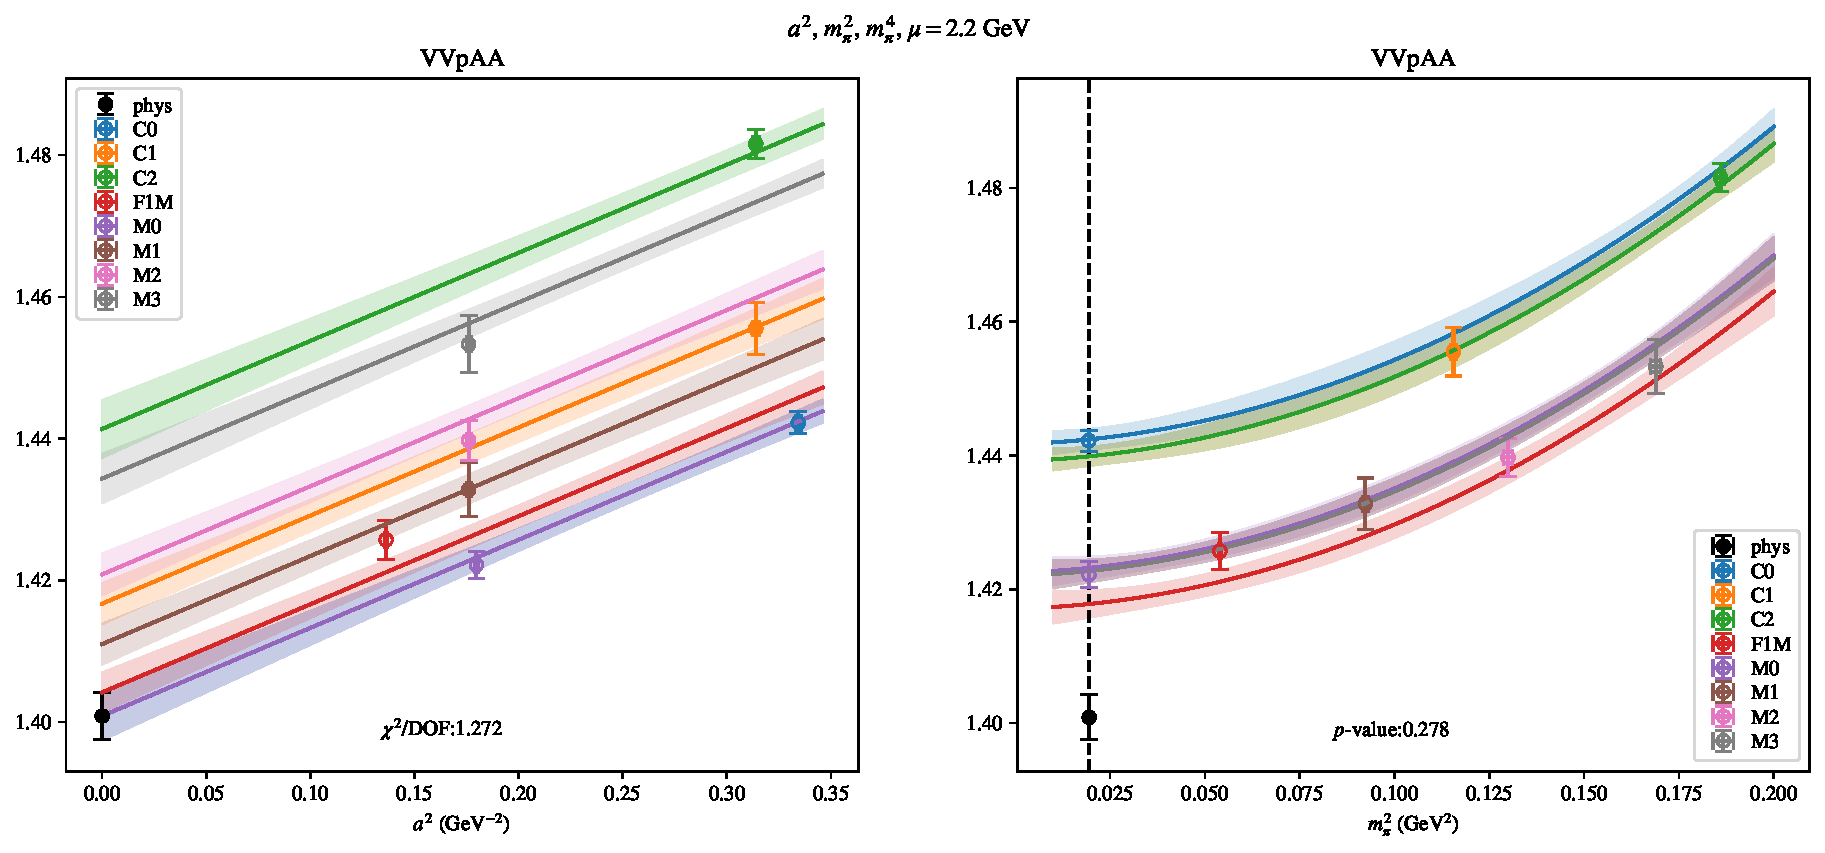
\includepdf[link, pages=-]{VVpAA/NPR/bag_a2m2m4_22.pdf}
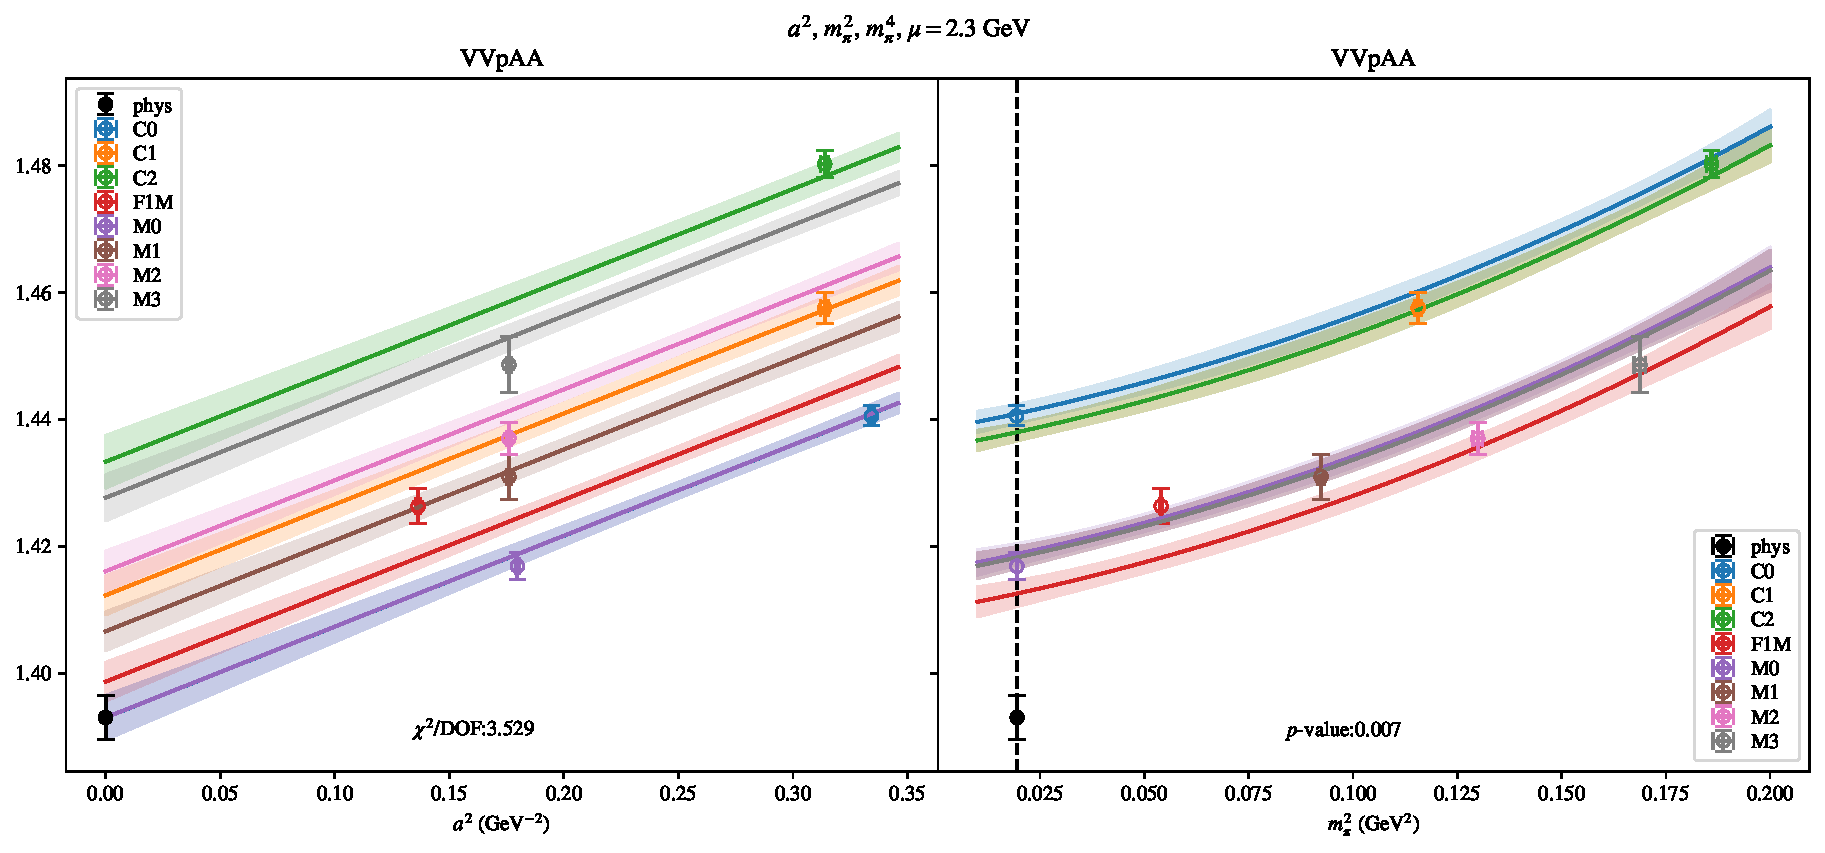
\includepdf[link, pages=-]{VVpAA/NPR/bag_a2m2m4_23.pdf}
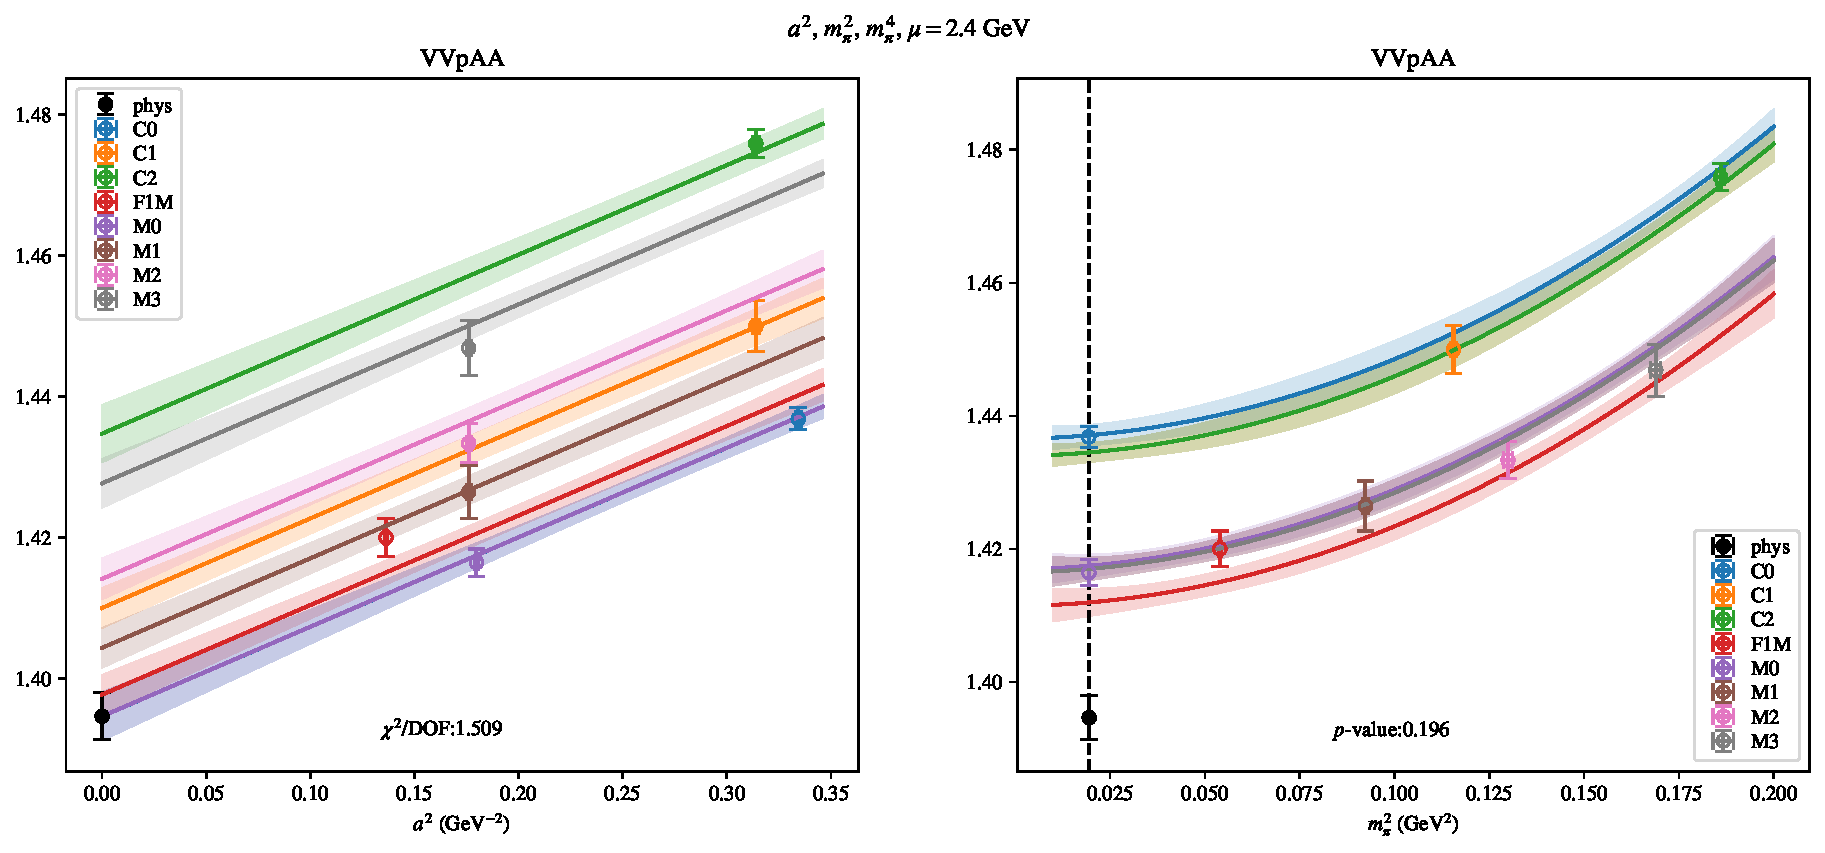
\includepdf[link, pages=-]{VVpAA/NPR/bag_a2m2m4_24.pdf}
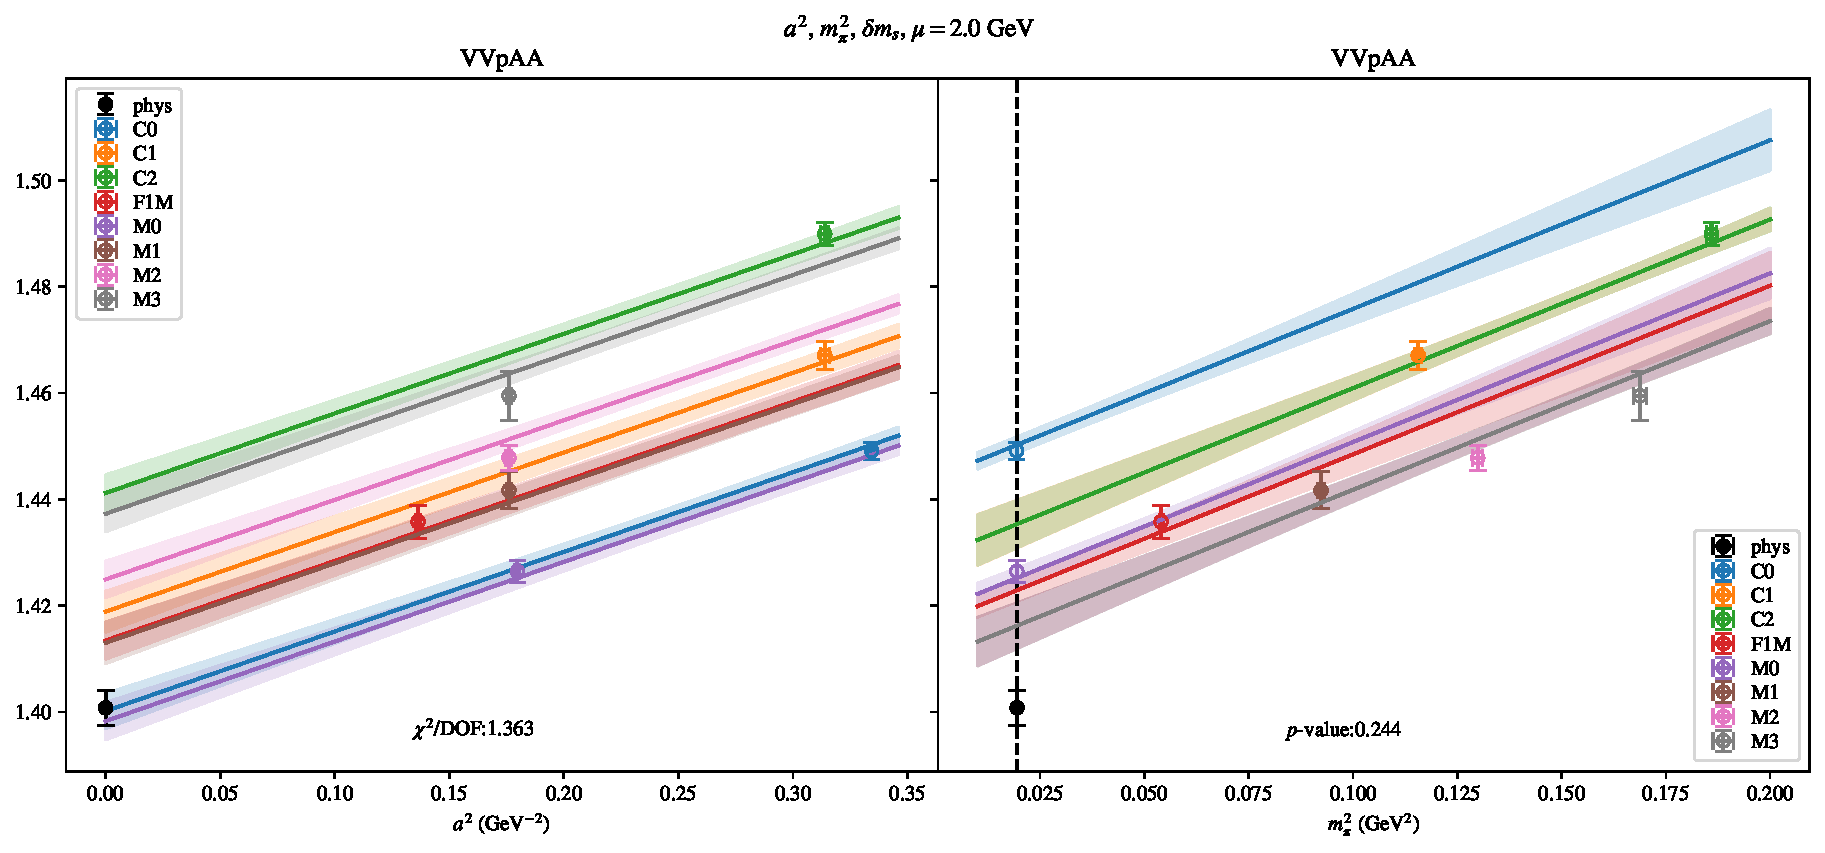
\includepdf[link, pages=-]{VVpAA/NPR/bag_a2m2delm_20.pdf}
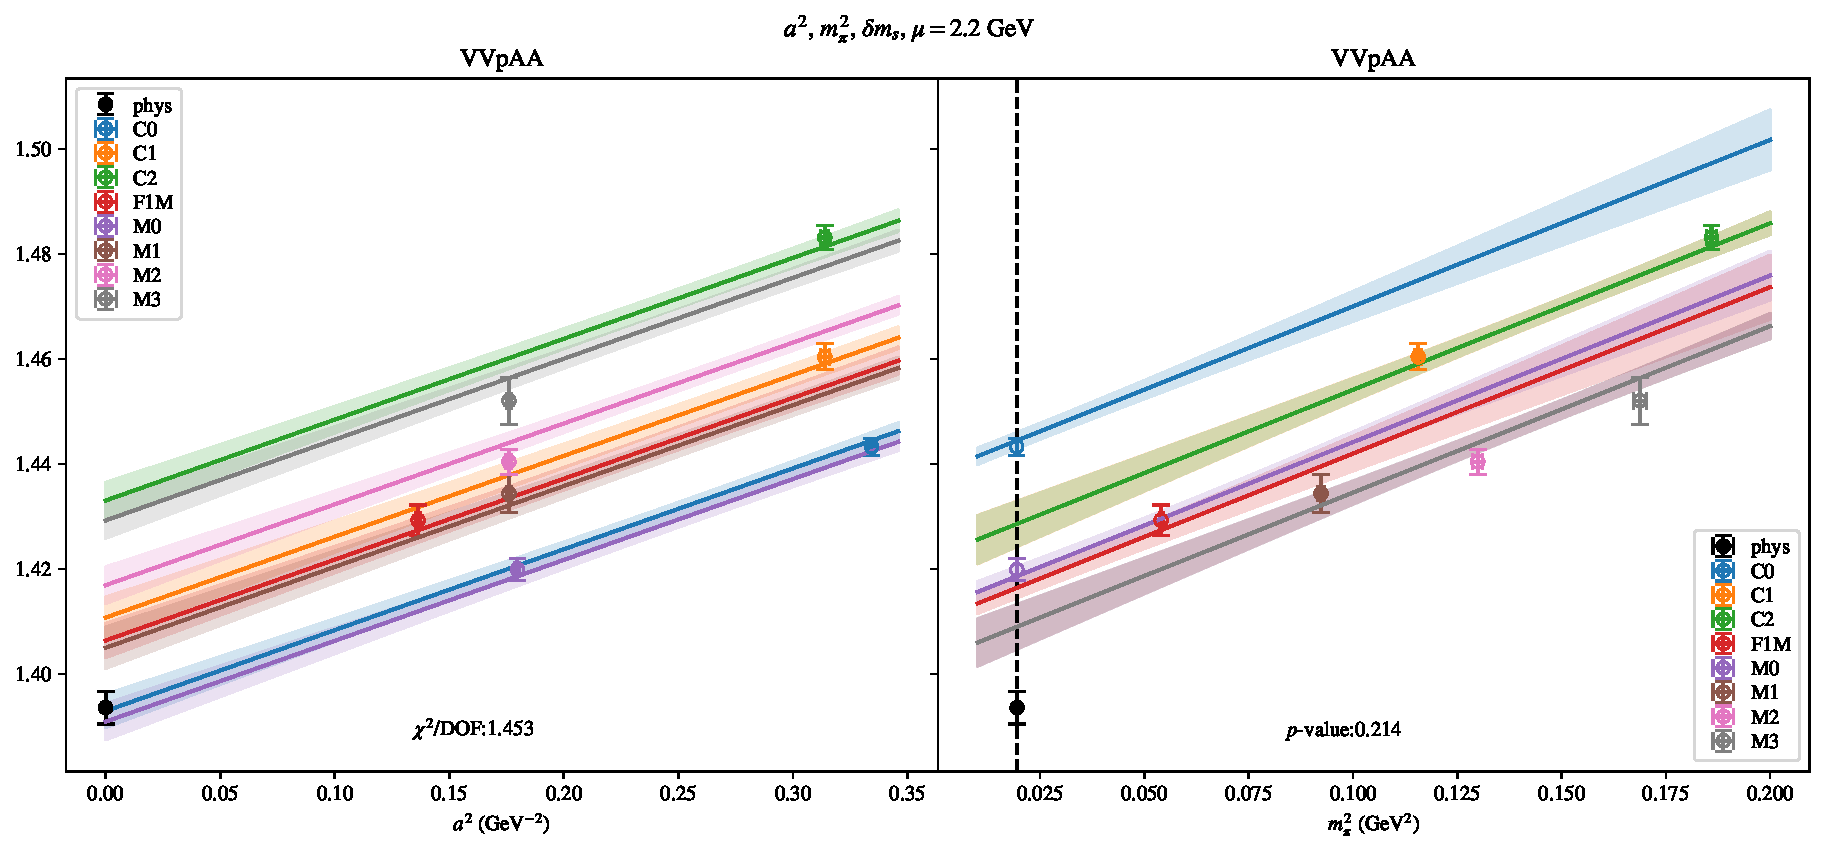
\includepdf[link, pages=-]{VVpAA/NPR/bag_a2m2delm_22.pdf}
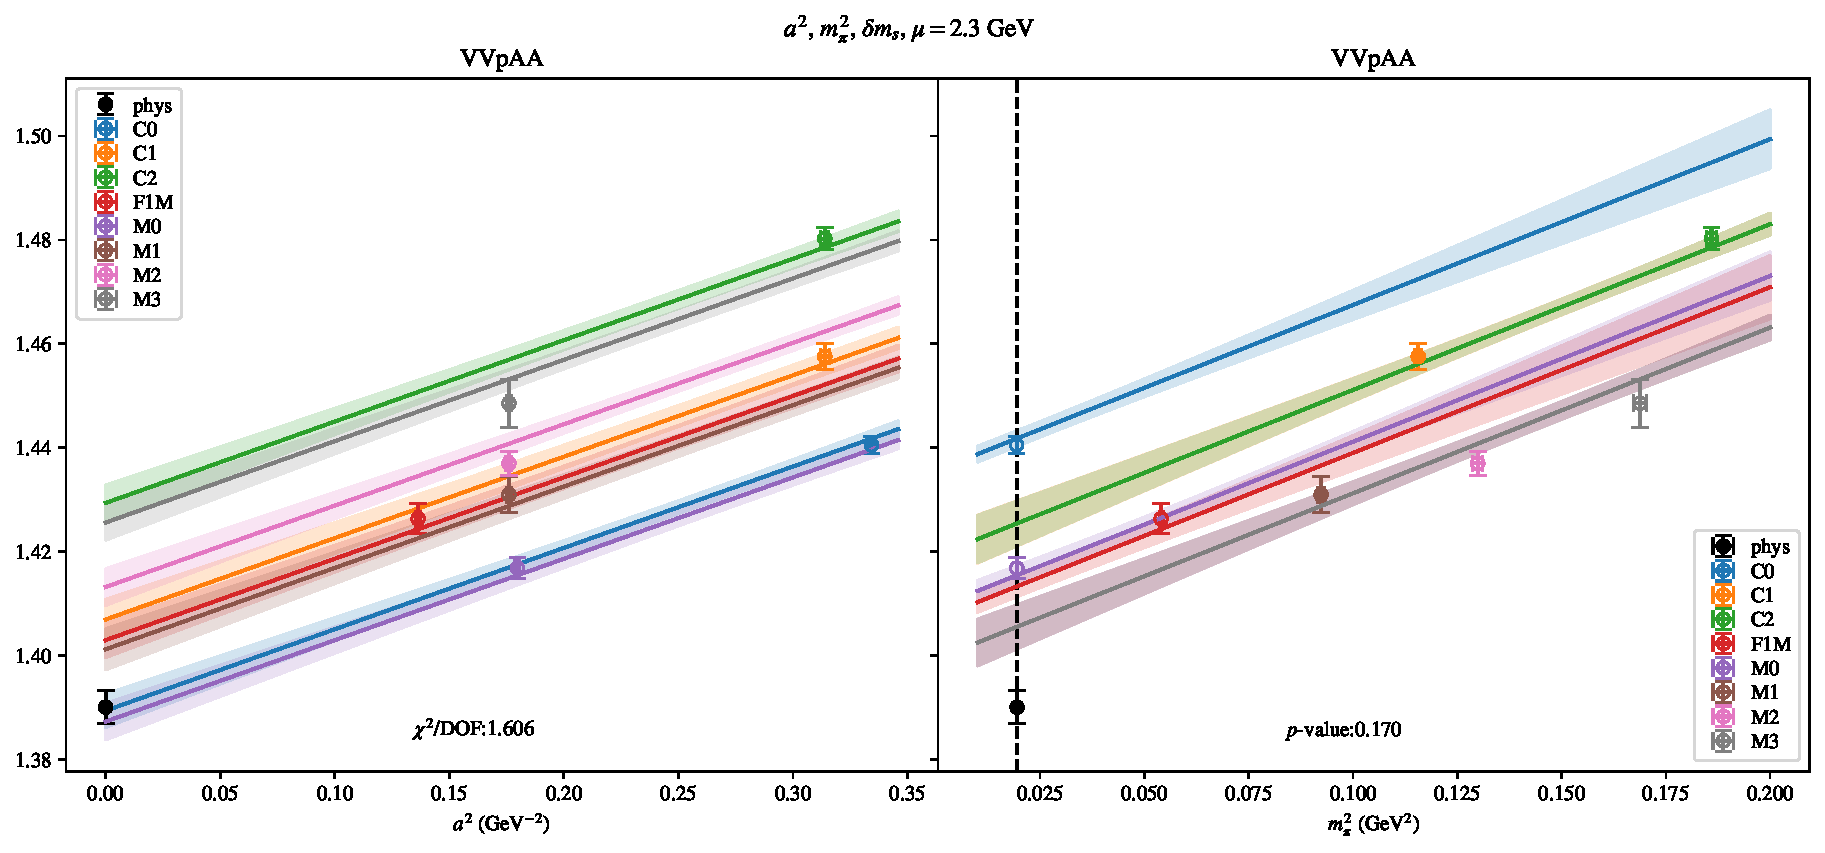
\includepdf[link, pages=-]{VVpAA/NPR/bag_a2m2delm_23.pdf}
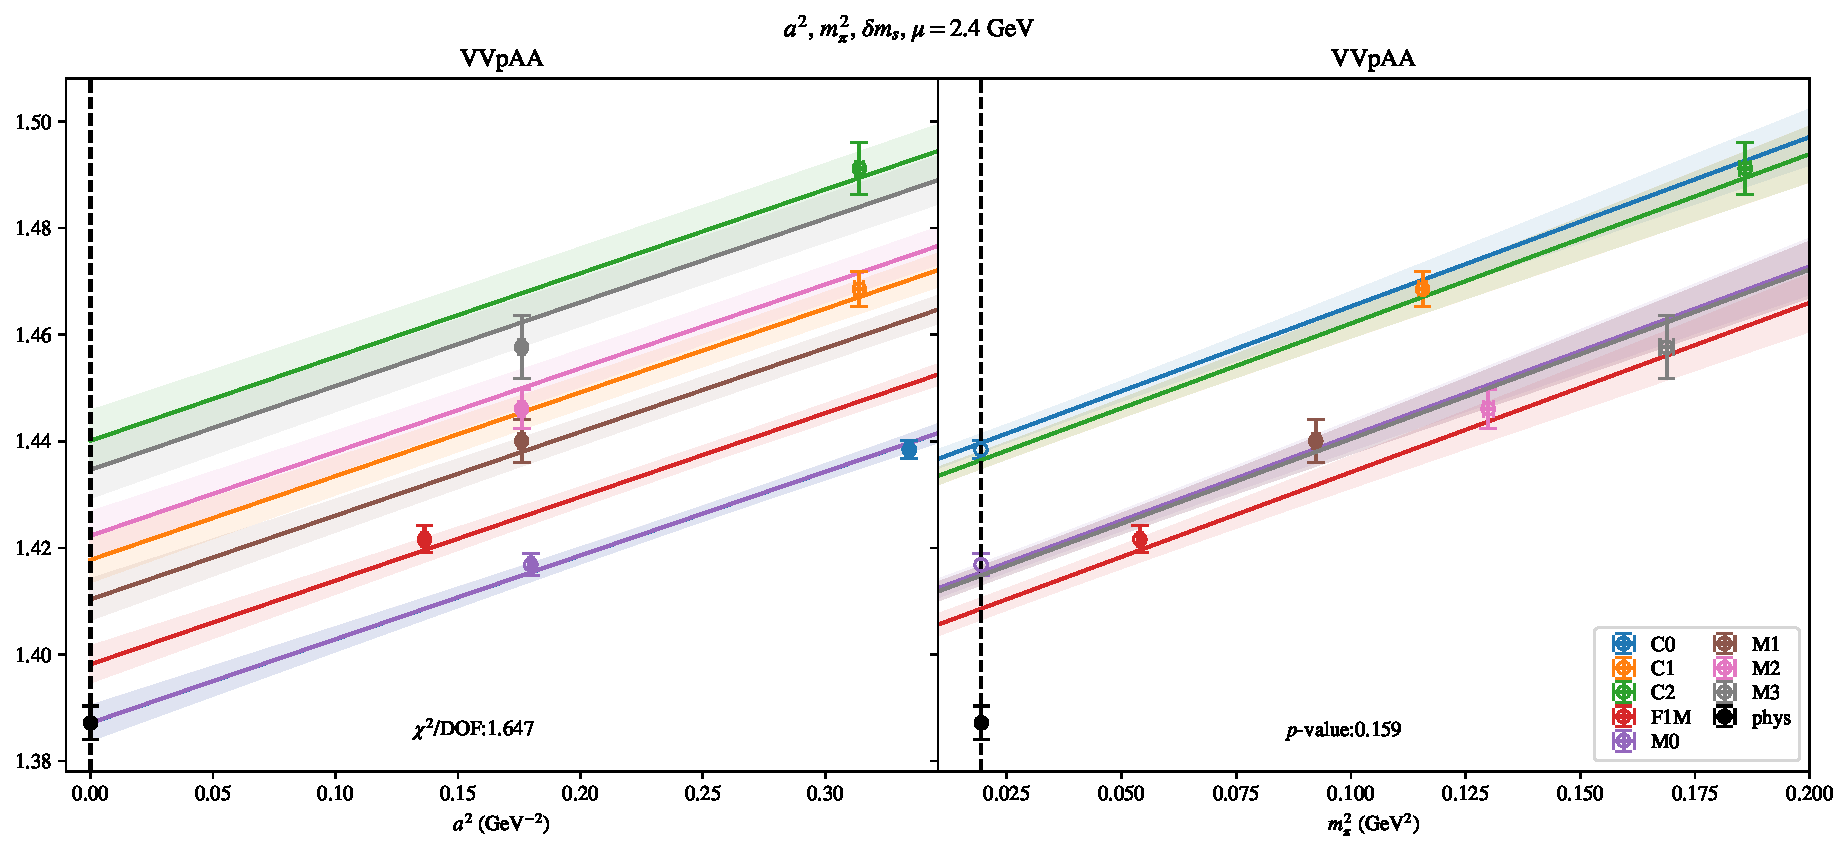
\includepdf[link, pages=-]{VVpAA/NPR/bag_a2m2delm_24.pdf}
\clearpage
\section{$\mathcal{B}_2$}
\begin{table}[h!]
\begin{center}
\begin{tabular}{|c|c|c|c|c|c|c|}
\hline
$\mu$ (GeV) & $a^2$, $m_\pi^2$& $a^2$, $m_\pi^2$ (no C)& $a^2$, $m_\pi^2$, $a^4$& $a^2$, $m_\pi^2$ (no M3, C2)& $a^2$, $m_\pi^2$, $m_\pi^4$& $a^2$, $m_\pi^2$, $\delta m_s$\\
\hline
2.0& \hyperlink{VVmAA/NPR/bag_a2m2_20.pdf.1}{\textbf{-0.9867(80)}: 0.345 (0.886)} & \hyperlink{VVmAA/NPR/bag_a2m2noC_20.pdf.1}{\textbf{-0.941(33)}: 0.081 (0.923)} & \hyperlink{VVmAA/NPR/bag_a2a4m2_20.pdf.1}{\textbf{-0.913(57)}: 0.118 (0.976)} & \hyperlink{VVmAA/NPR/bag_a2m2mcut_20.pdf.1}{\textbf{-0.9854(88)}: 0.669 (0.571)} & \hyperlink{VVmAA/NPR/bag_a2m2m4_20.pdf.1}{\textbf{-0.9877(92)}: 0.456 (0.768)} & \hyperlink{VVmAA/NPR/bag_a2m2delm_20.pdf.1}{\textbf{-0.9861(83)}: 0.322 (0.864)}\\
2.2& \hyperlink{VVmAA/NPR/bag_a2m2_22.pdf.1}{\textbf{-1.0007(64)}: 0.339 (0.89)} & \hyperlink{VVmAA/NPR/bag_a2m2noC_22.pdf.1}{\textbf{-0.961(30)}: 0.049 (0.952)} & \hyperlink{VVmAA/NPR/bag_a2a4m2_22.pdf.1}{\textbf{-0.940(52)}: 0.14 (0.968)} & \hyperlink{VVmAA/NPR/bag_a2m2mcut_22.pdf.1}{\textbf{-1.0014(83)}: 0.552 (0.647)} & \hyperlink{VVmAA/NPR/bag_a2m2m4_22.pdf.1}{\textbf{-1.0023(78)}: 0.37 (0.83)} & \hyperlink{VVmAA/NPR/bag_a2m2delm_22.pdf.1}{\textbf{-1.0005(74)}: 0.376 (0.826)}\\
2.3& \hyperlink{VVmAA/NPR/bag_a2m2_23.pdf.1}{\textbf{-1.0074(63)}: 0.385 (0.859)} & \hyperlink{VVmAA/NPR/bag_a2m2noC_23.pdf.1}{\textbf{-0.968(29)}: 0.052 (0.95)} & \hyperlink{VVmAA/NPR/bag_a2a4m2_23.pdf.1}{\textbf{-0.946(46)}: 0.128 (0.972)} & \hyperlink{VVmAA/NPR/bag_a2m2mcut_23.pdf.1}{\textbf{-1.0077(75)}: 0.59 (0.621)} & \hyperlink{VVmAA/NPR/bag_a2m2m4_23.pdf.1}{\textbf{-1.0081(75)}: 0.373 (0.828)} & \hyperlink{VVmAA/NPR/bag_a2m2delm_23.pdf.1}{\textbf{-1.0067(68)}: 0.378 (0.825)}\\
2.4& \hyperlink{VVmAA/NPR/bag_a2m2_24.pdf.1}{\textbf{-1.0118(59)}: 0.397 (0.851)} & \hyperlink{VVmAA/NPR/bag_a2m2noC_24.pdf.1}{\textbf{-0.975(28)}: 0.053 (0.949)} & \hyperlink{VVmAA/NPR/bag_a2a4m2_24.pdf.1}{\textbf{-0.955(46)}: 0.143 (0.966)} & \hyperlink{VVmAA/NPR/bag_a2m2mcut_24.pdf.1}{\textbf{-1.0120(69)}: 0.658 (0.578)} & \hyperlink{VVmAA/NPR/bag_a2m2m4_24.pdf.1}{\textbf{-1.0138(69)}: 0.413 (0.799)} & \hyperlink{VVmAA/NPR/bag_a2m2delm_24.pdf.1}{\textbf{-1.0120(58)}: 0.454 (0.769)}\\
\hline
\end{tabular}
\caption{Physical point value from chiral and continuum extrapolation at renormalisation scale $\mu$. Entries are \textbf{value(error)}: $\chi^2/\text{DOF}$ ($p$-value).}
\end{center}
\end{table}
\begin{table}[h!]
\begin{center}
\begin{tabular}{|c c|c|c|c|c|c|c|}
\hline
$\mu$ (GeV) &  & $a^2$, $m_\pi^2$& $a^2$, $m_\pi^2$ (no C)& $a^2$, $m_\pi^2$, $a^4$& $a^2$, $m_\pi^2$ (no M3, C2)& $a^2$, $m_\pi^2$, $m_\pi^4$& $a^2$, $m_\pi^2$, $\delta m_s$\\
\hline
\multirow{3}{0.5in}{2.0} & $\alpha$ & 0.169(28)& -0.10(19)& -0.51(53)& 0.165(30)& 0.172(30)& 0.169(28)\\
 & $\beta$ & -0.00147(53)& -0.0013(10)& -0.00108(58)& -0.00148(96)& -0.0006(29)& -0.0007(12)\\
 & $\gamma$ &  &  & 1.4(10)&  & -0.00008(24)& -0.031(45)\\
\hline
\multirow{3}{0.5in}{2.2} & $\alpha$ & 0.212(22)& -0.03(18)& -0.35(47)& 0.214(28)& 0.217(25)& 0.214(25)\\
 & $\beta$ & -0.00160(45)& -0.00138(92)& -0.00126(54)& -0.00137(77)& -0.0003(21)& -0.0012(10)\\
 & $\gamma$ &  &  & 1.14(97)&  & -0.00012(18)& -0.018(39)\\
\hline
\multirow{3}{0.5in}{2.3} & $\alpha$ & 0.238(21)& 0.001(172)& -0.33(43)& 0.238(25)& 0.239(24)& 0.237(24)\\
 & $\beta$ & -0.00156(39)& -0.00138(89)& -0.00123(47)& -0.00139(74)& -0.0005(21)& -0.0010(10)\\
 & $\gamma$ &  &  & 1.15(88)&  & -0.00009(17)& -0.021(39)\\
\hline
\multirow{3}{0.5in}{2.4} & $\alpha$ & 0.258(20)& 0.04(16)& -0.27(43)& 0.258(23)& 0.263(22)& 0.260(20)\\
 & $\beta$ & -0.00154(37)& -0.00139(76)& -0.00121(46)& -0.00141(66)& -0.0005(18)& -0.00106(90)\\
 & $\gamma$ &  &  & 1.07(87)&  & -0.00009(16)& -0.019(31)\\
\hline
\end{tabular}
\caption{Fit values of coefficients in $Q = Q_{phys} + \mathbf{\alpha} a^2 + \mathbf{\beta}\left(\frac{m_\pi^2}{f_\pi^2}-\frac{m_{\pi,PDG}^2}{f_\pi^2}\right) + \gamma(\ldots)$}
\end{center}
\end{table}
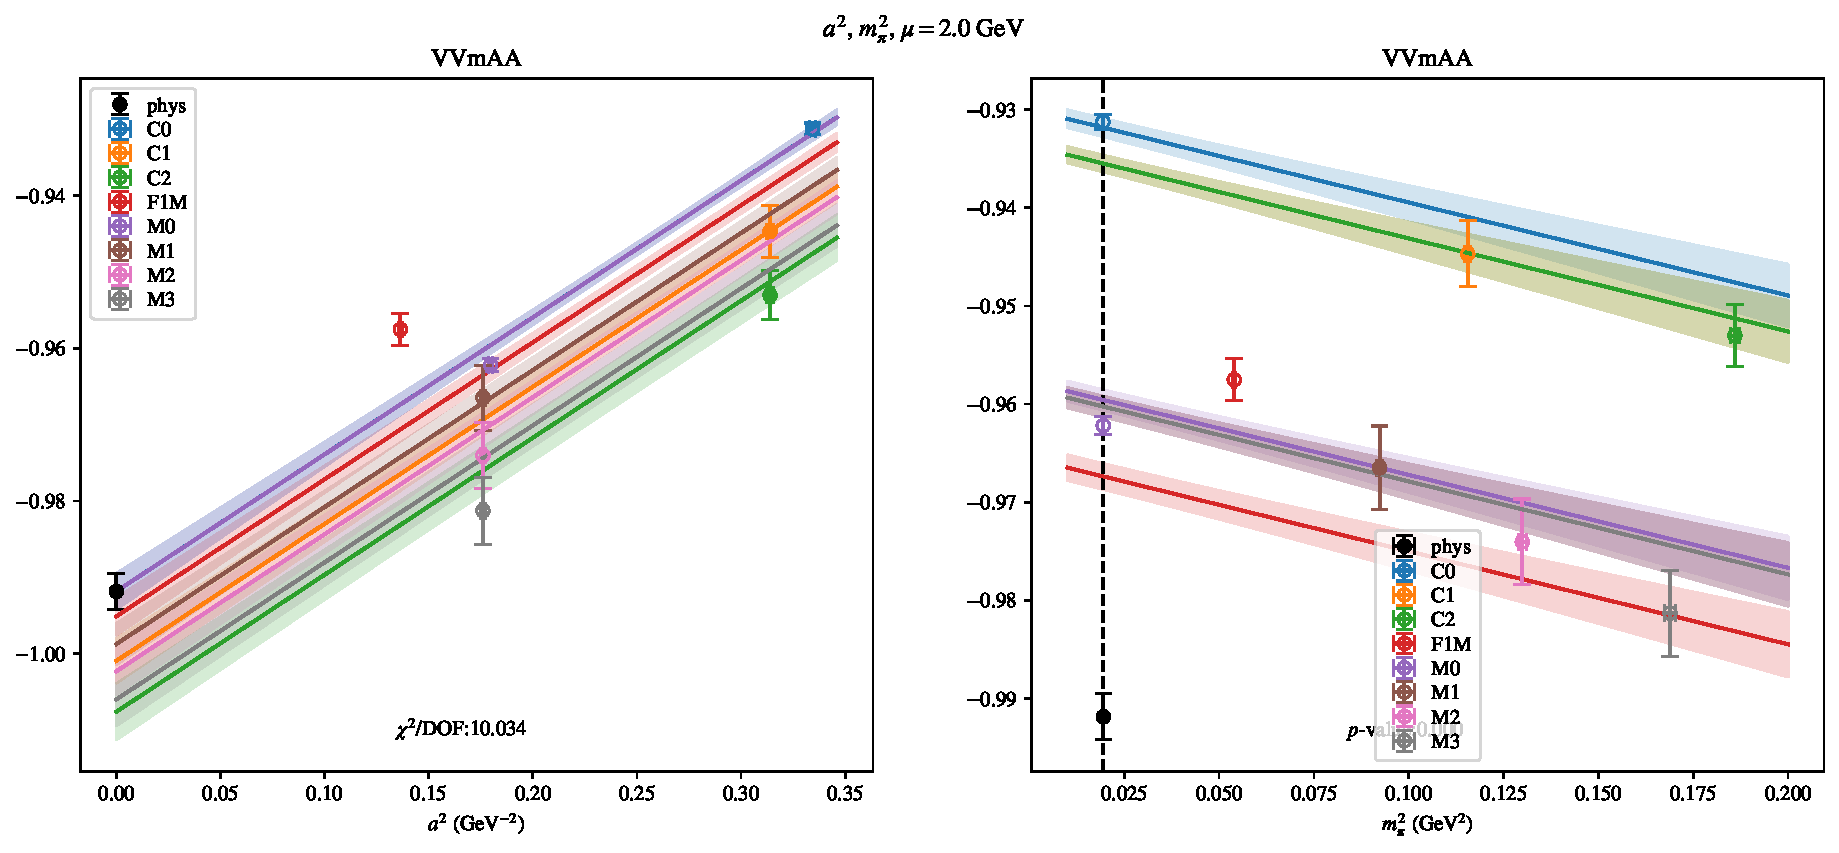
\includepdf[link, pages=-]{VVmAA/NPR/bag_a2m2_20.pdf}
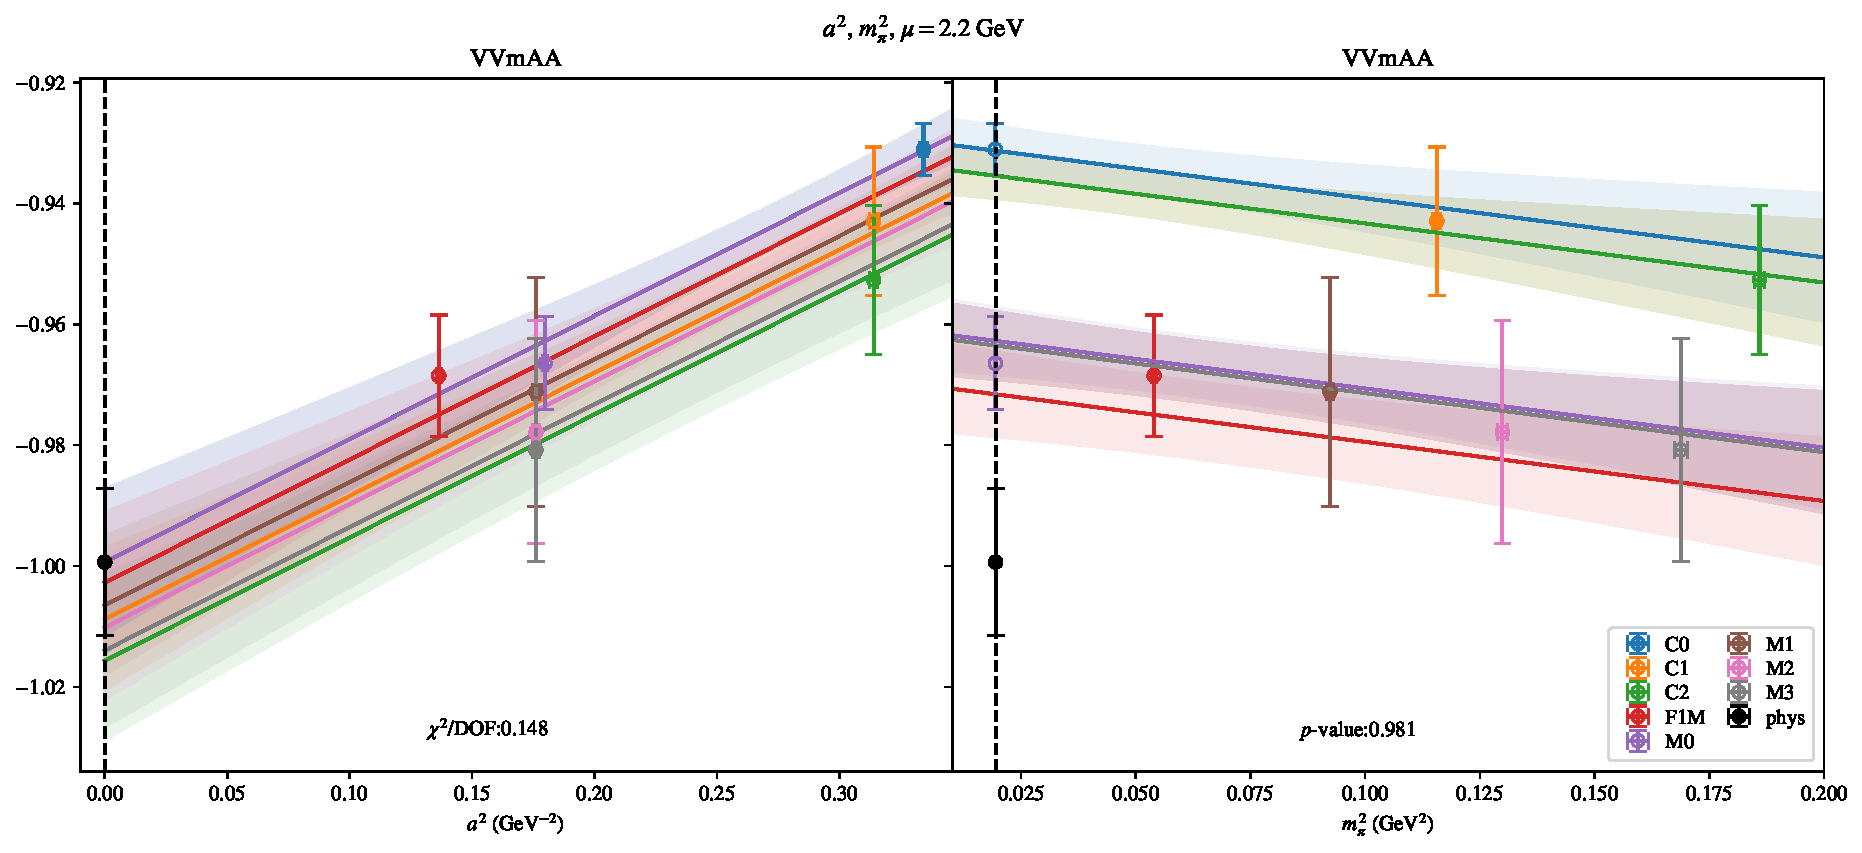
\includepdf[link, pages=-]{VVmAA/NPR/bag_a2m2_22.pdf}
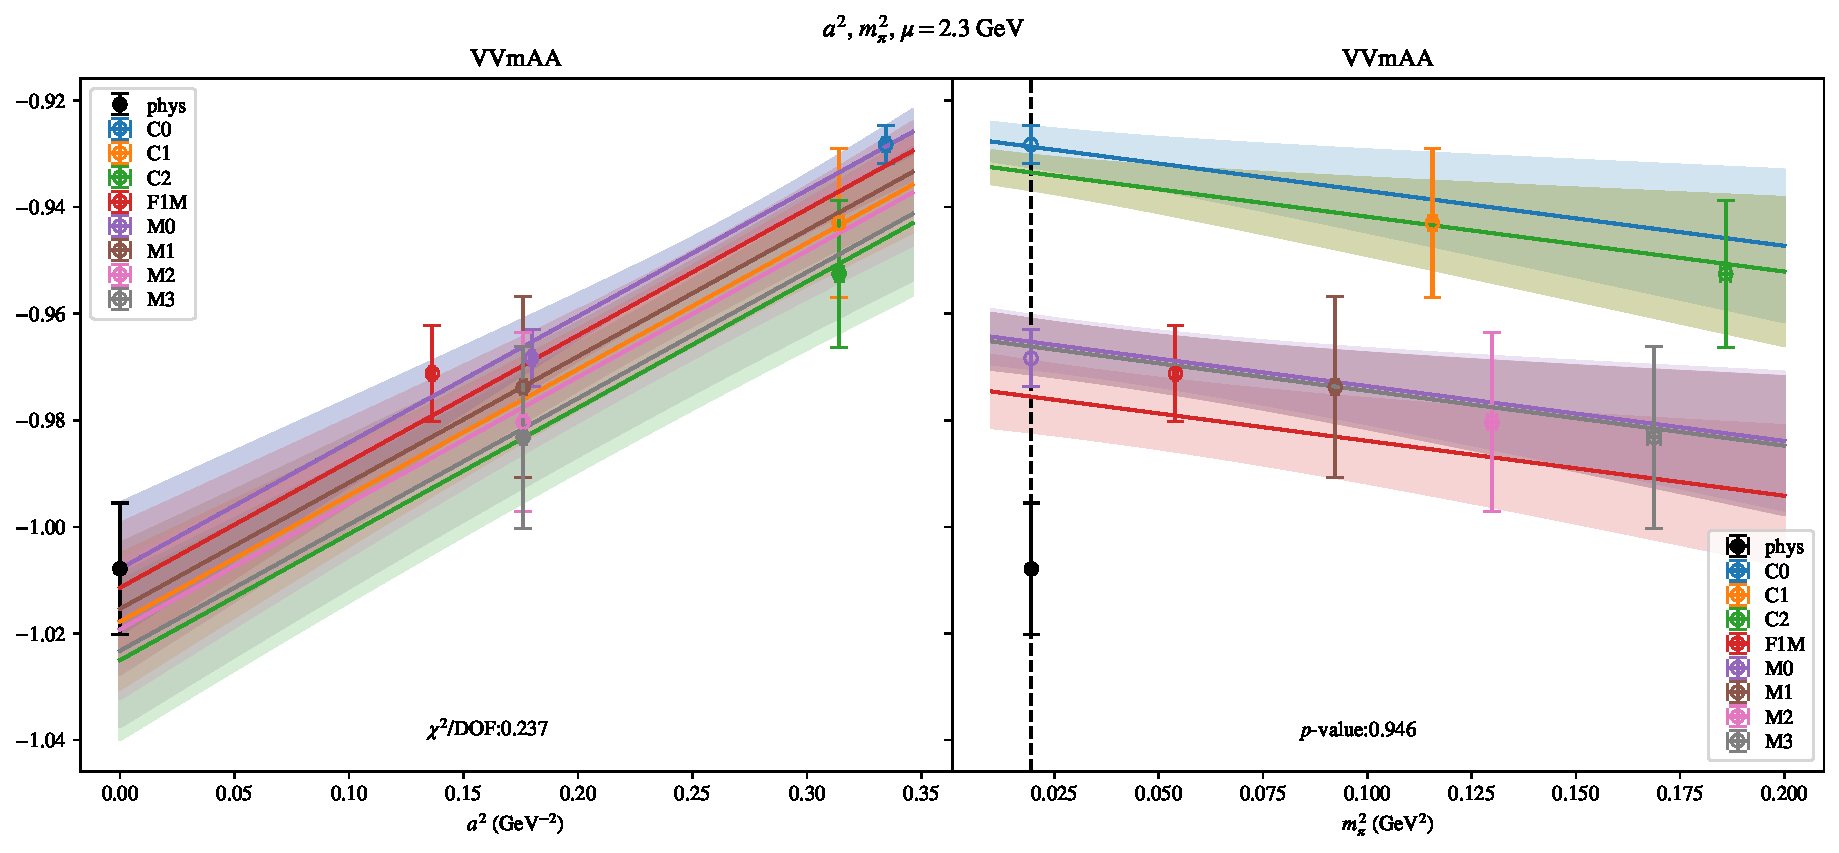
\includepdf[link, pages=-]{VVmAA/NPR/bag_a2m2_23.pdf}
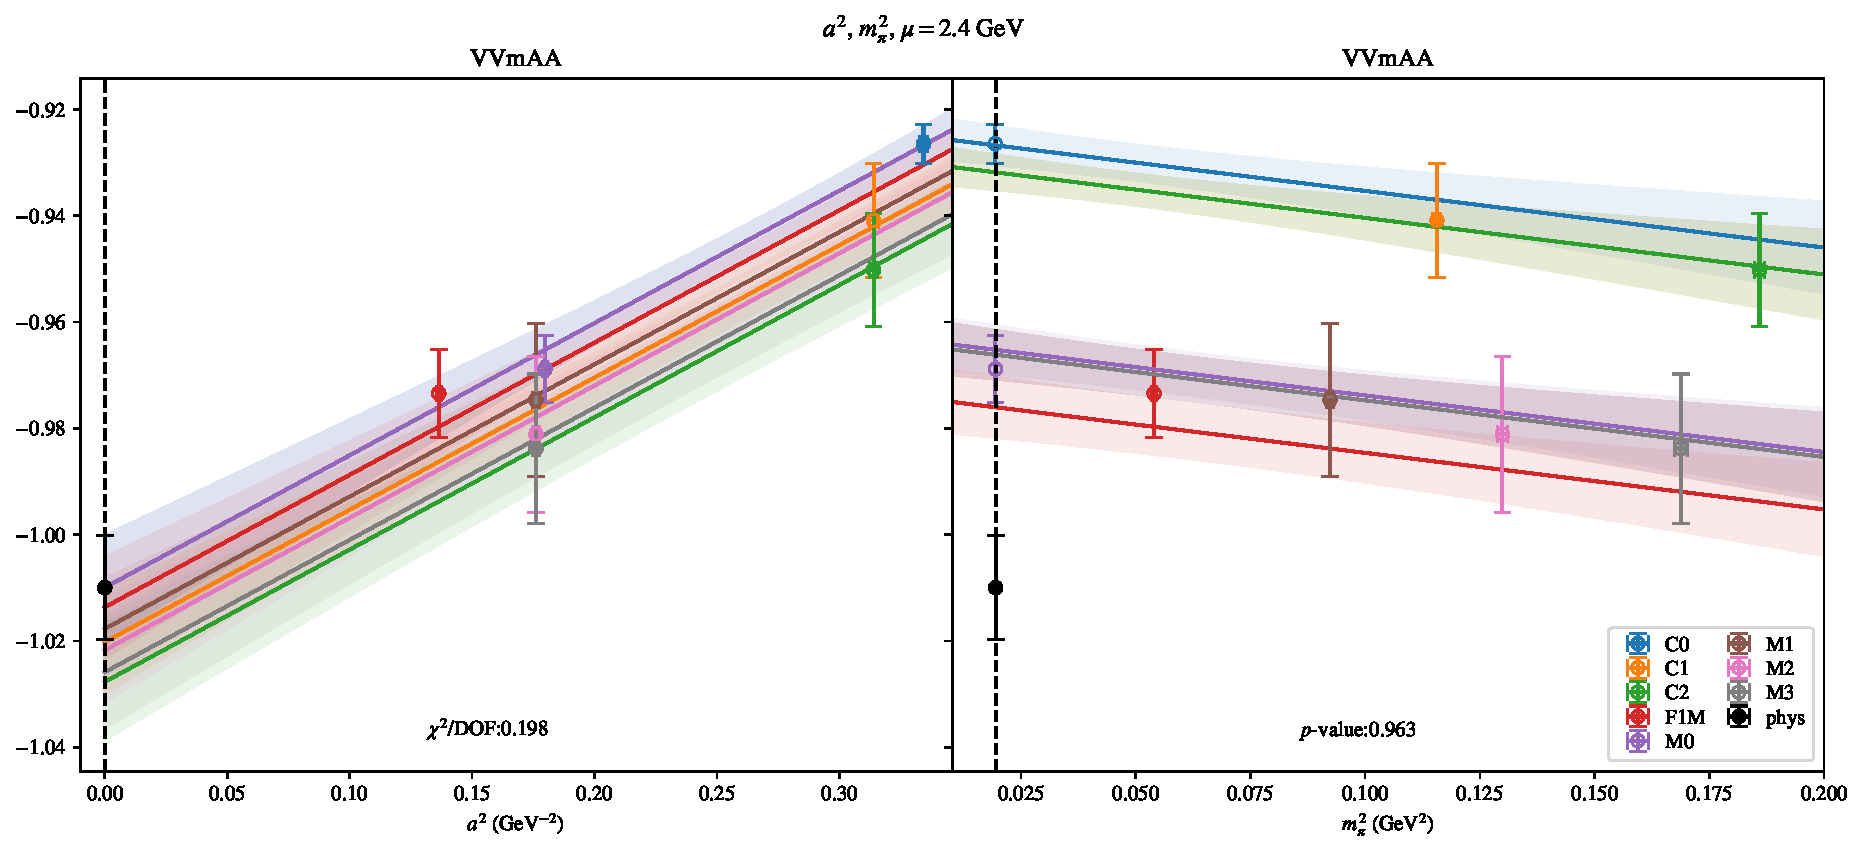
\includepdf[link, pages=-]{VVmAA/NPR/bag_a2m2_24.pdf}
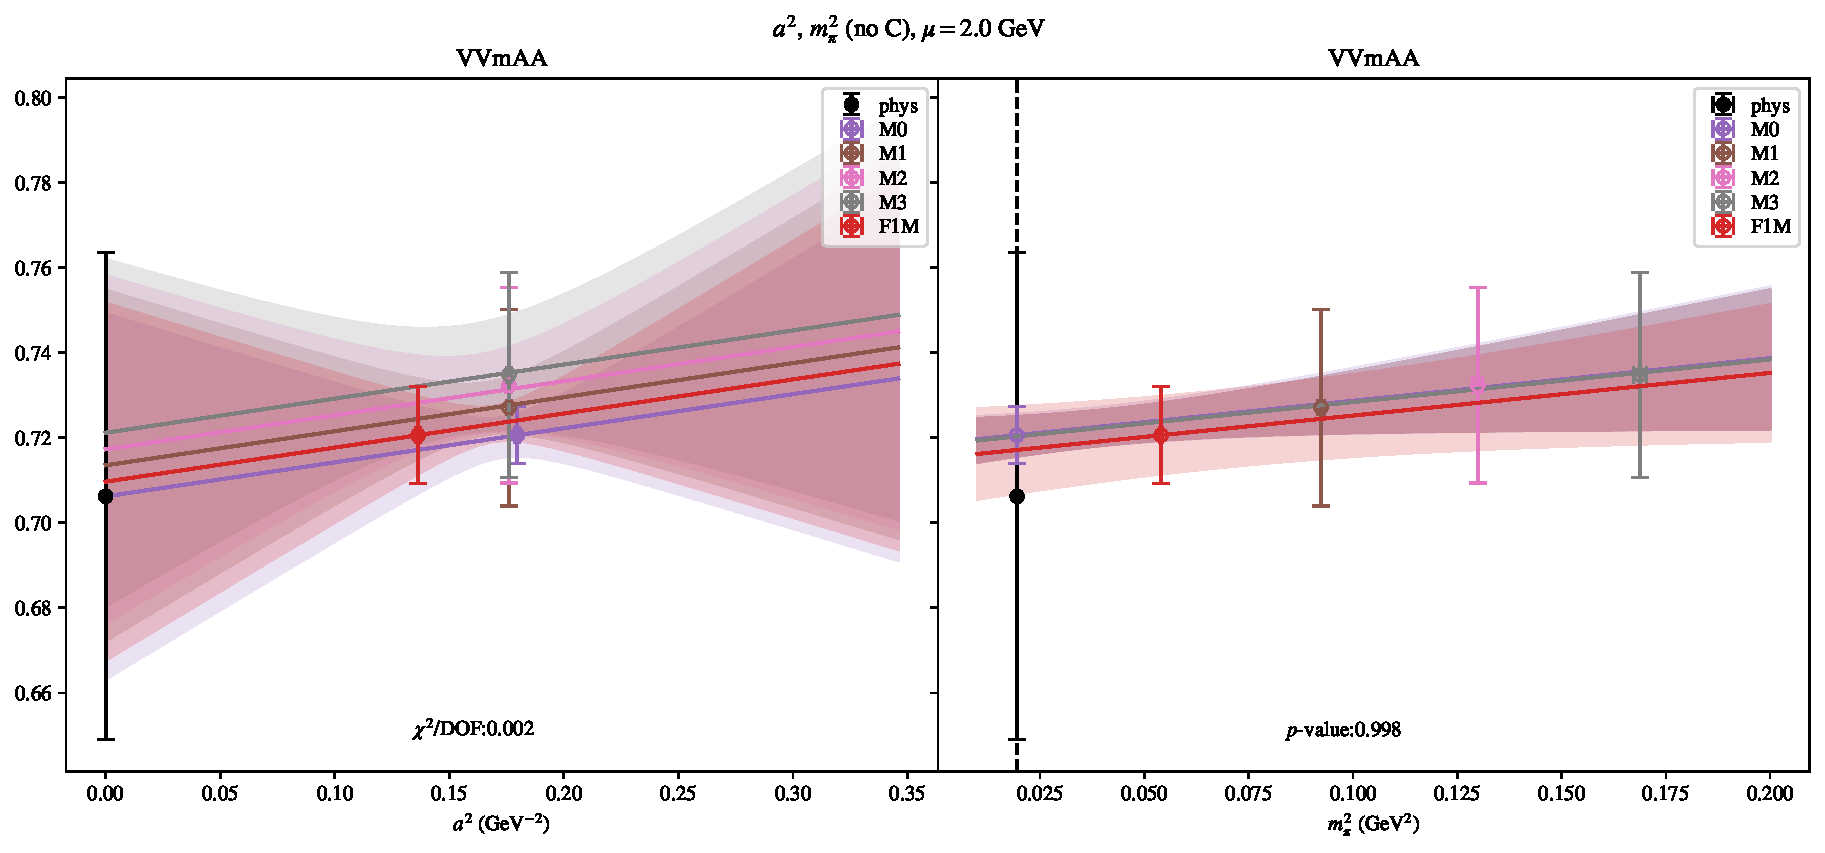
\includepdf[link, pages=-]{VVmAA/NPR/bag_a2m2noC_20.pdf}
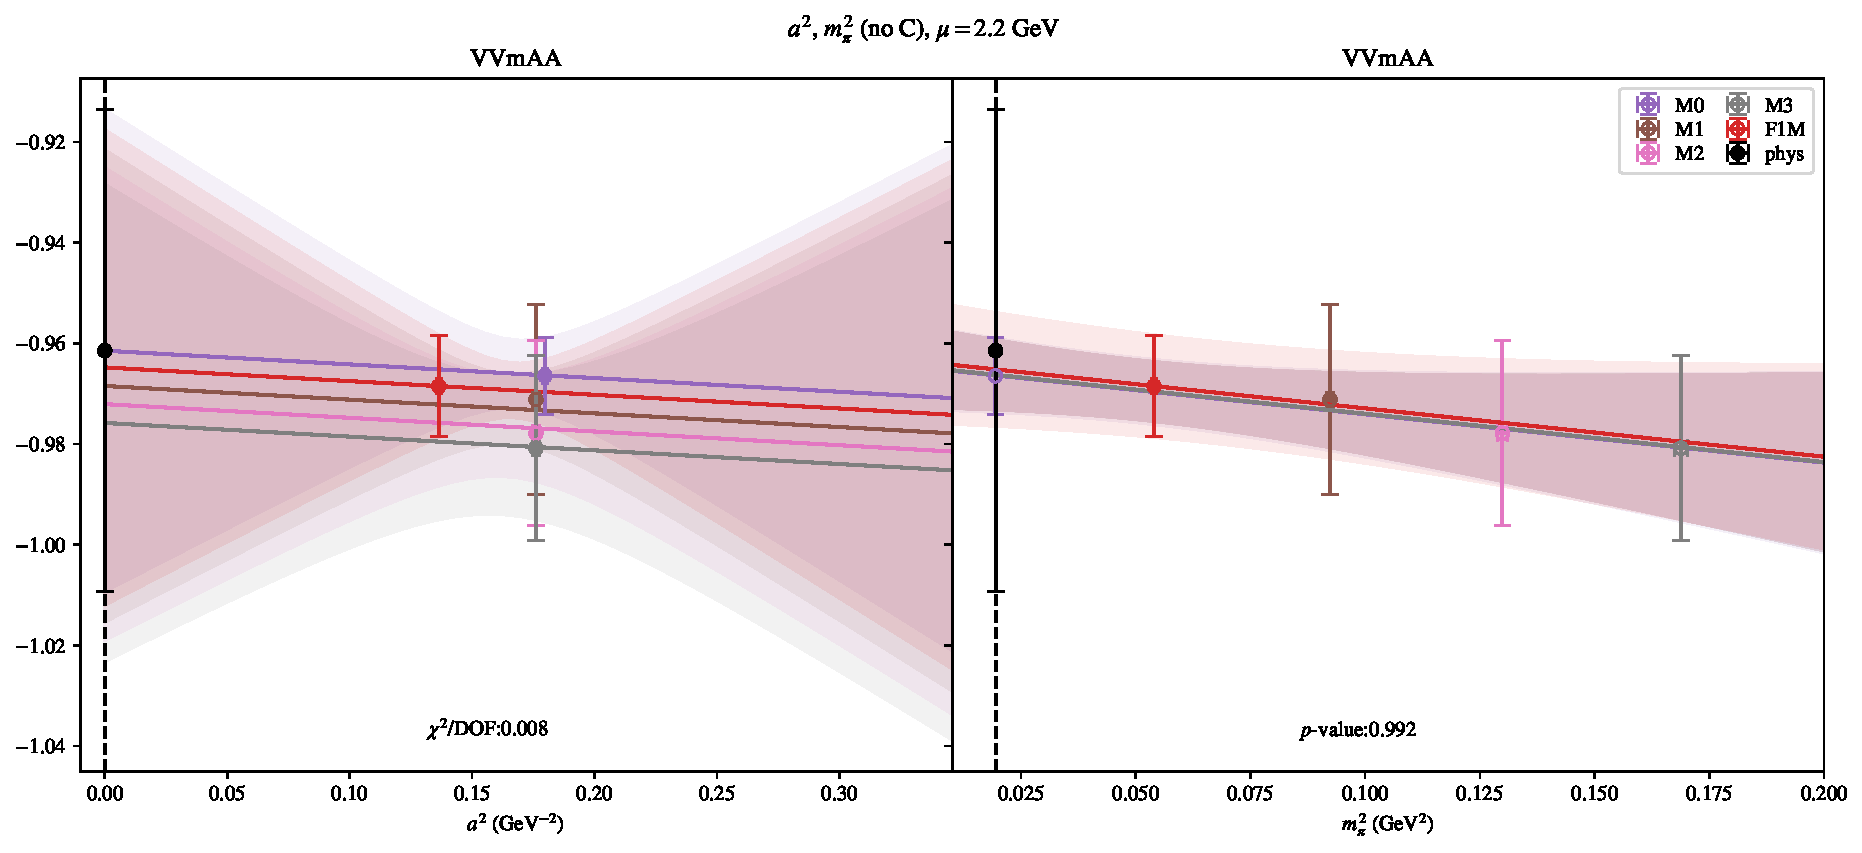
\includepdf[link, pages=-]{VVmAA/NPR/bag_a2m2noC_22.pdf}
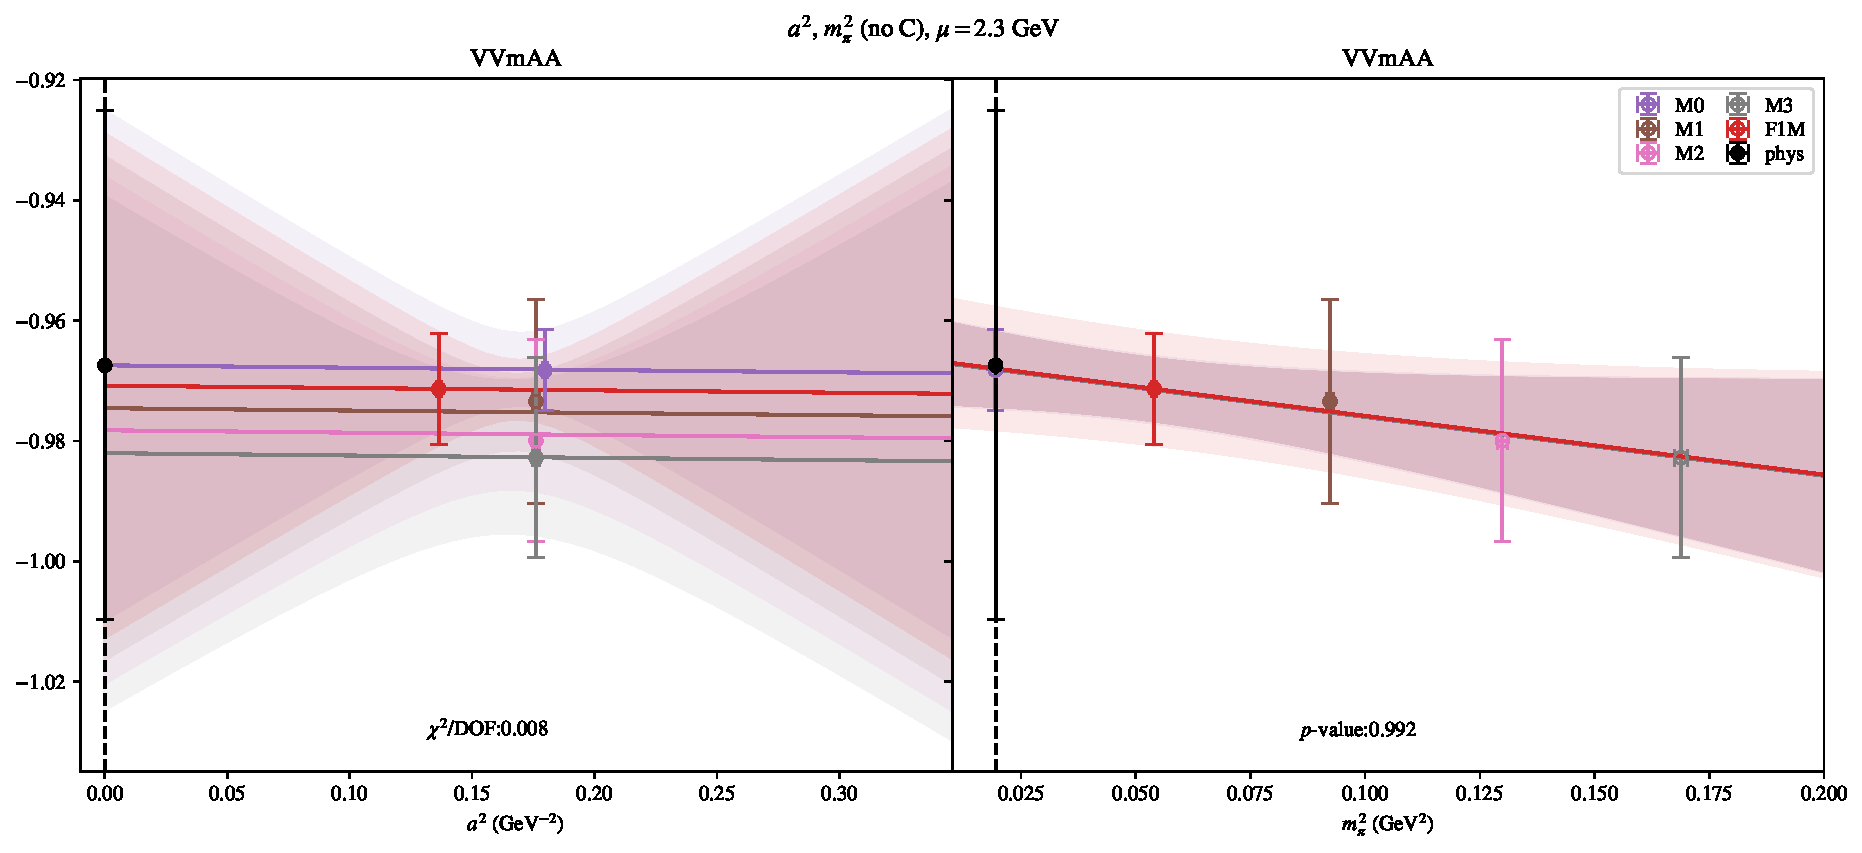
\includepdf[link, pages=-]{VVmAA/NPR/bag_a2m2noC_23.pdf}
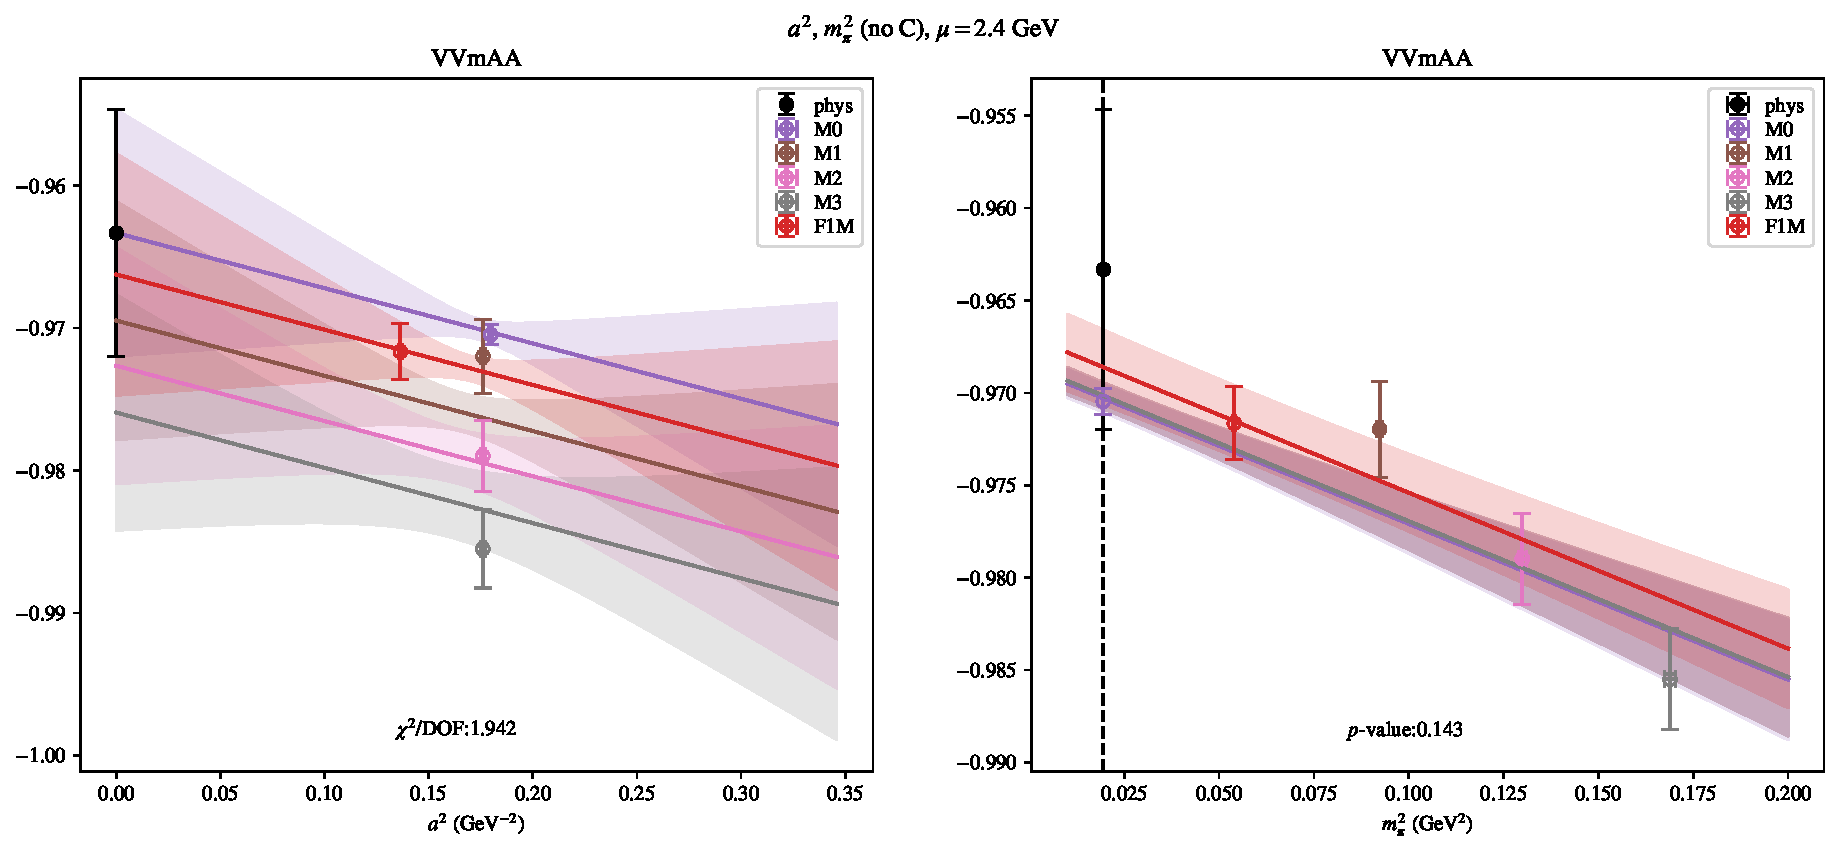
\includepdf[link, pages=-]{VVmAA/NPR/bag_a2m2noC_24.pdf}
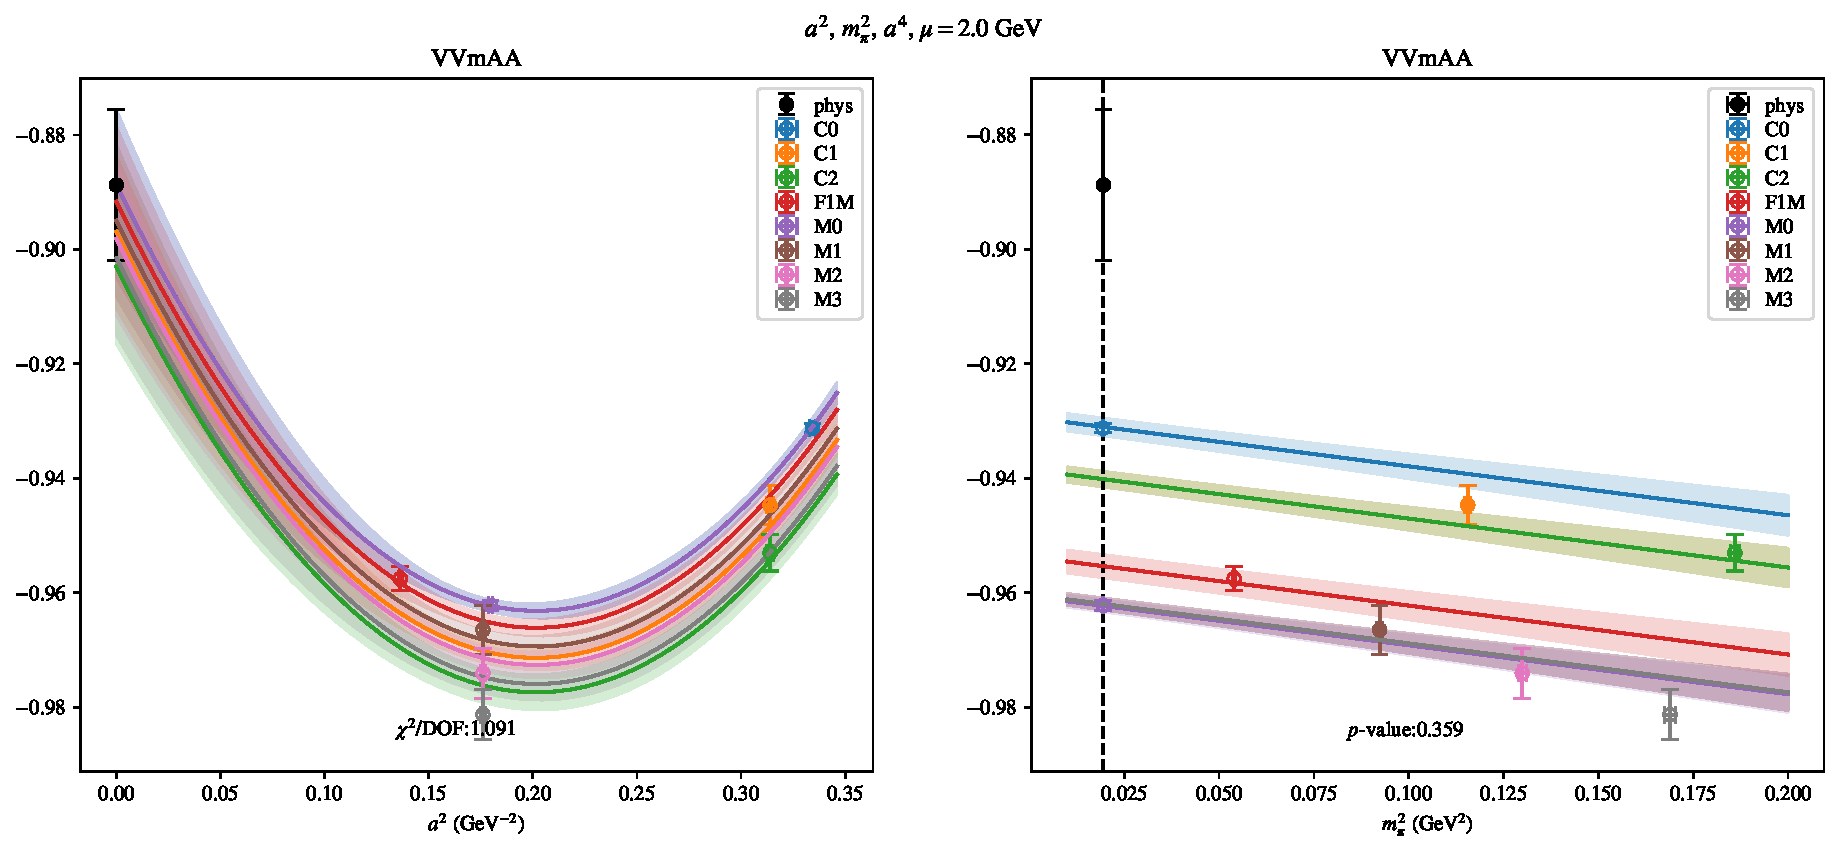
\includepdf[link, pages=-]{VVmAA/NPR/bag_a2a4m2_20.pdf}
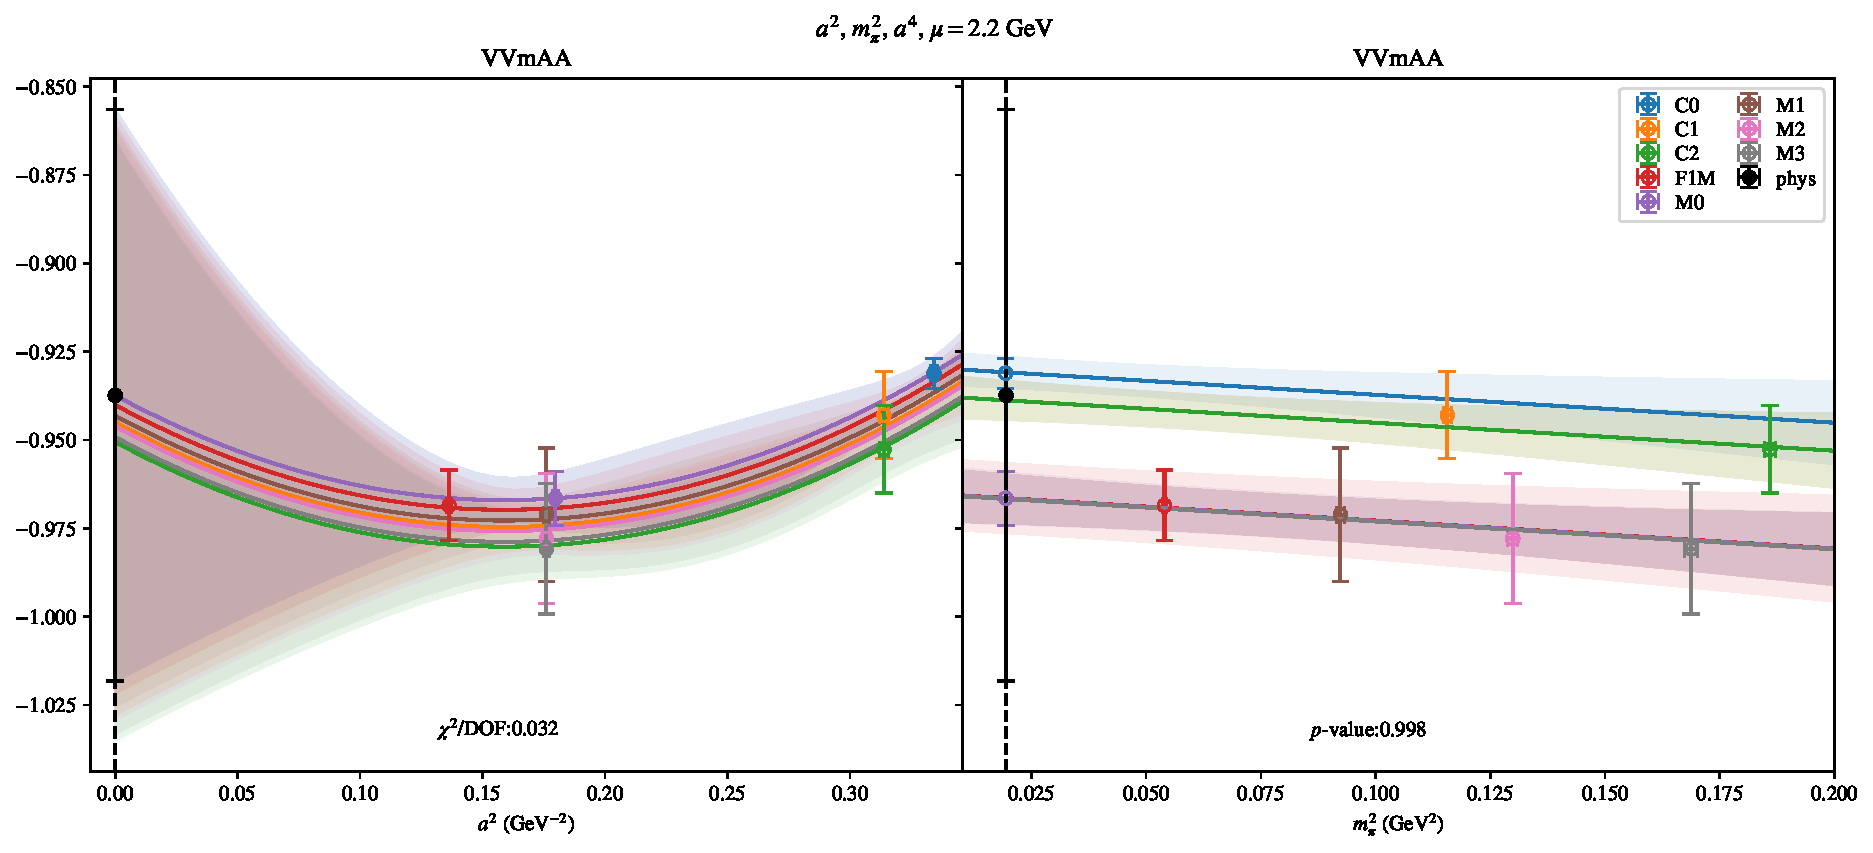
\includepdf[link, pages=-]{VVmAA/NPR/bag_a2a4m2_22.pdf}
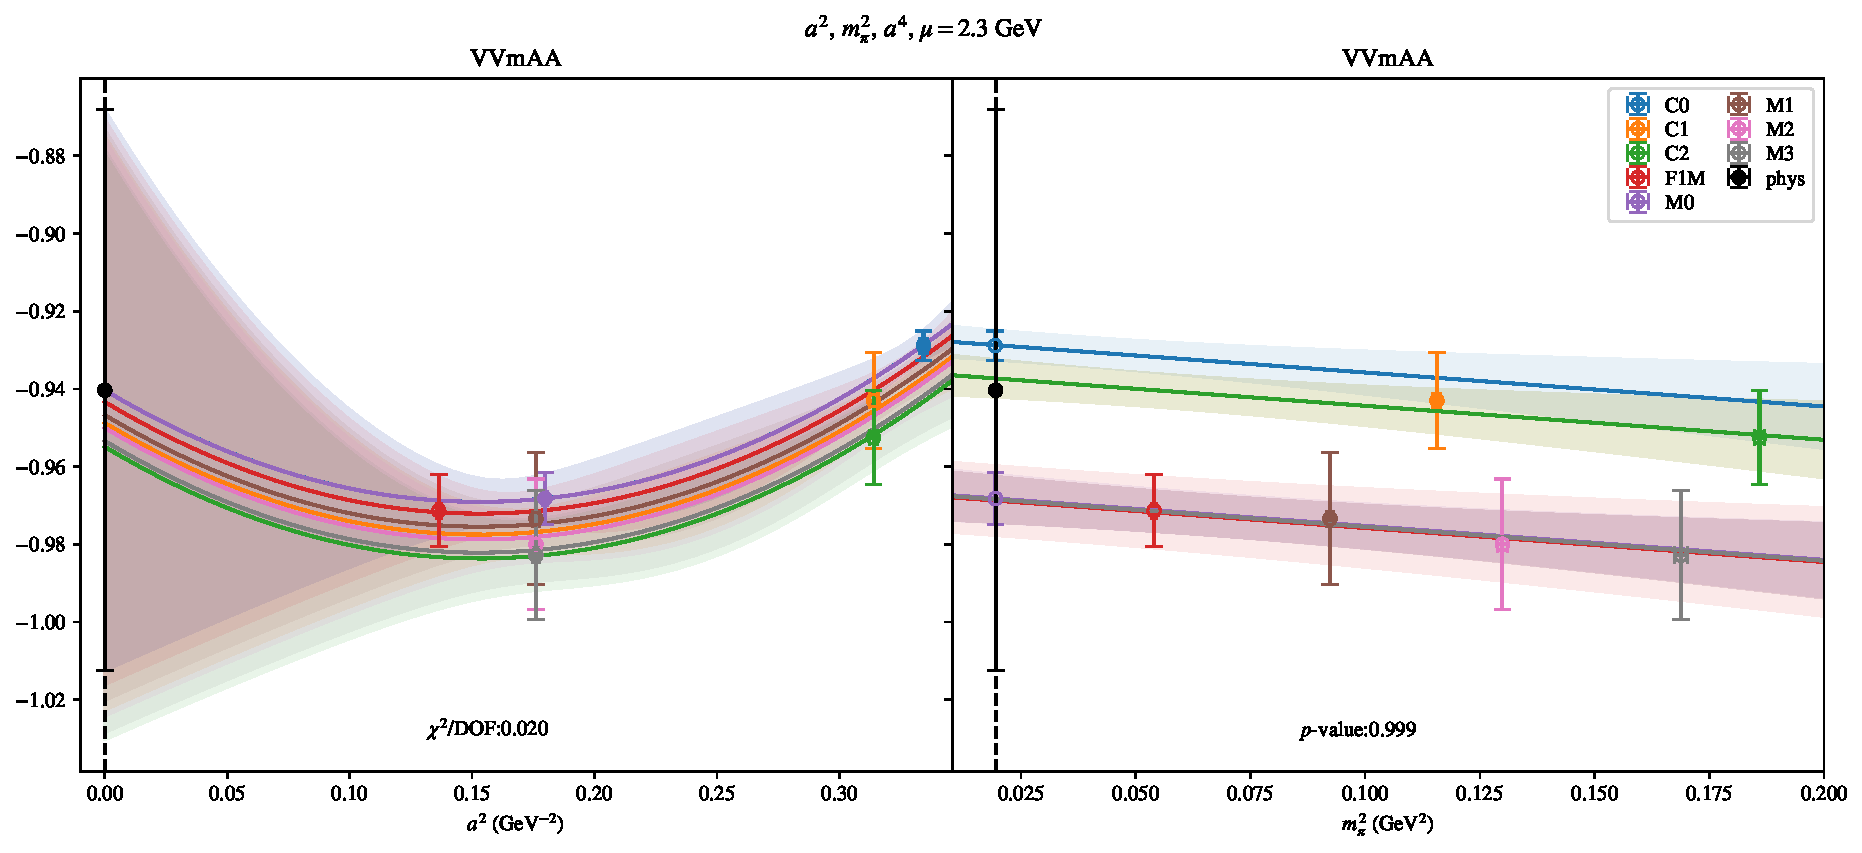
\includepdf[link, pages=-]{VVmAA/NPR/bag_a2a4m2_23.pdf}
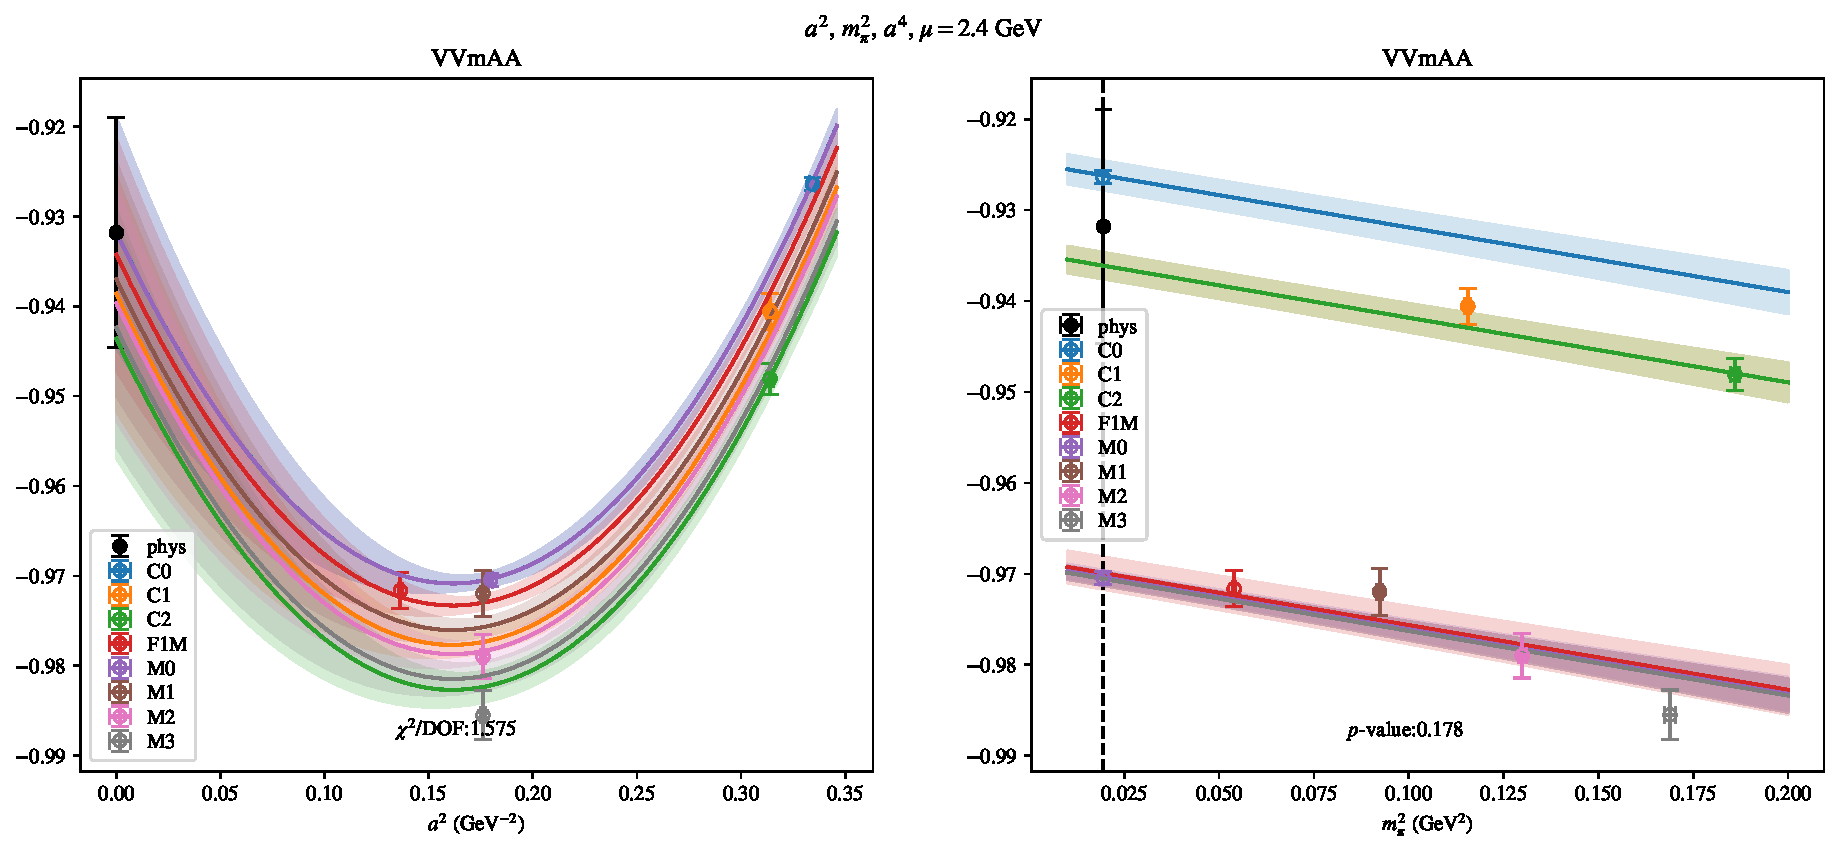
\includepdf[link, pages=-]{VVmAA/NPR/bag_a2a4m2_24.pdf}
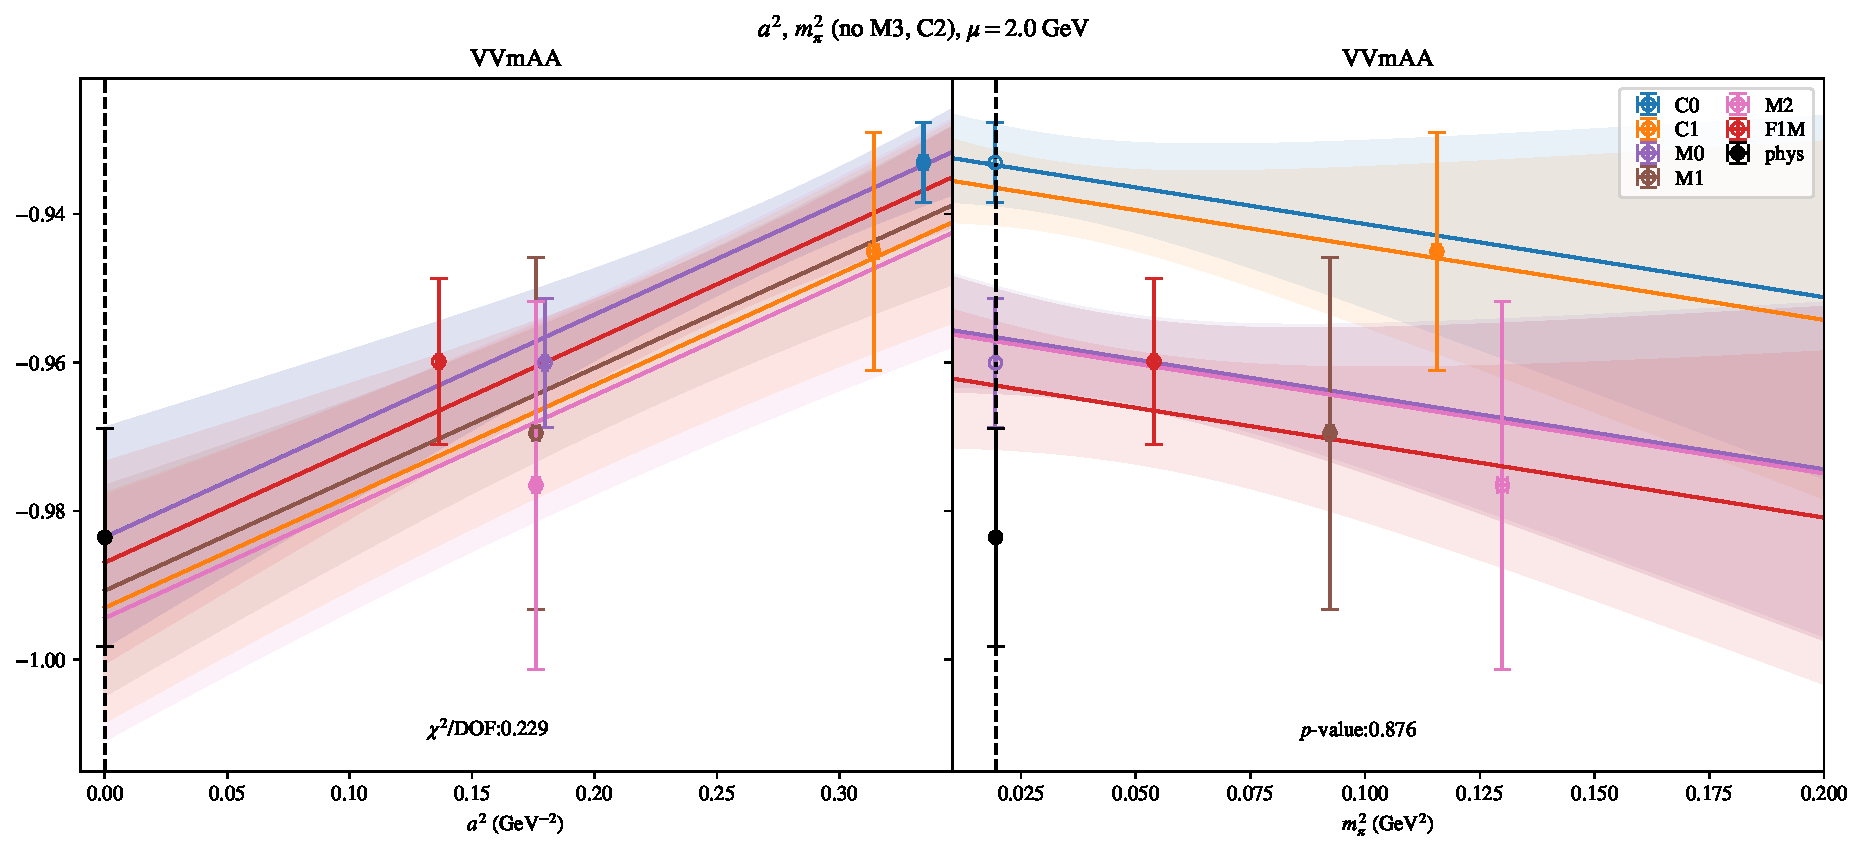
\includepdf[link, pages=-]{VVmAA/NPR/bag_a2m2mcut_20.pdf}
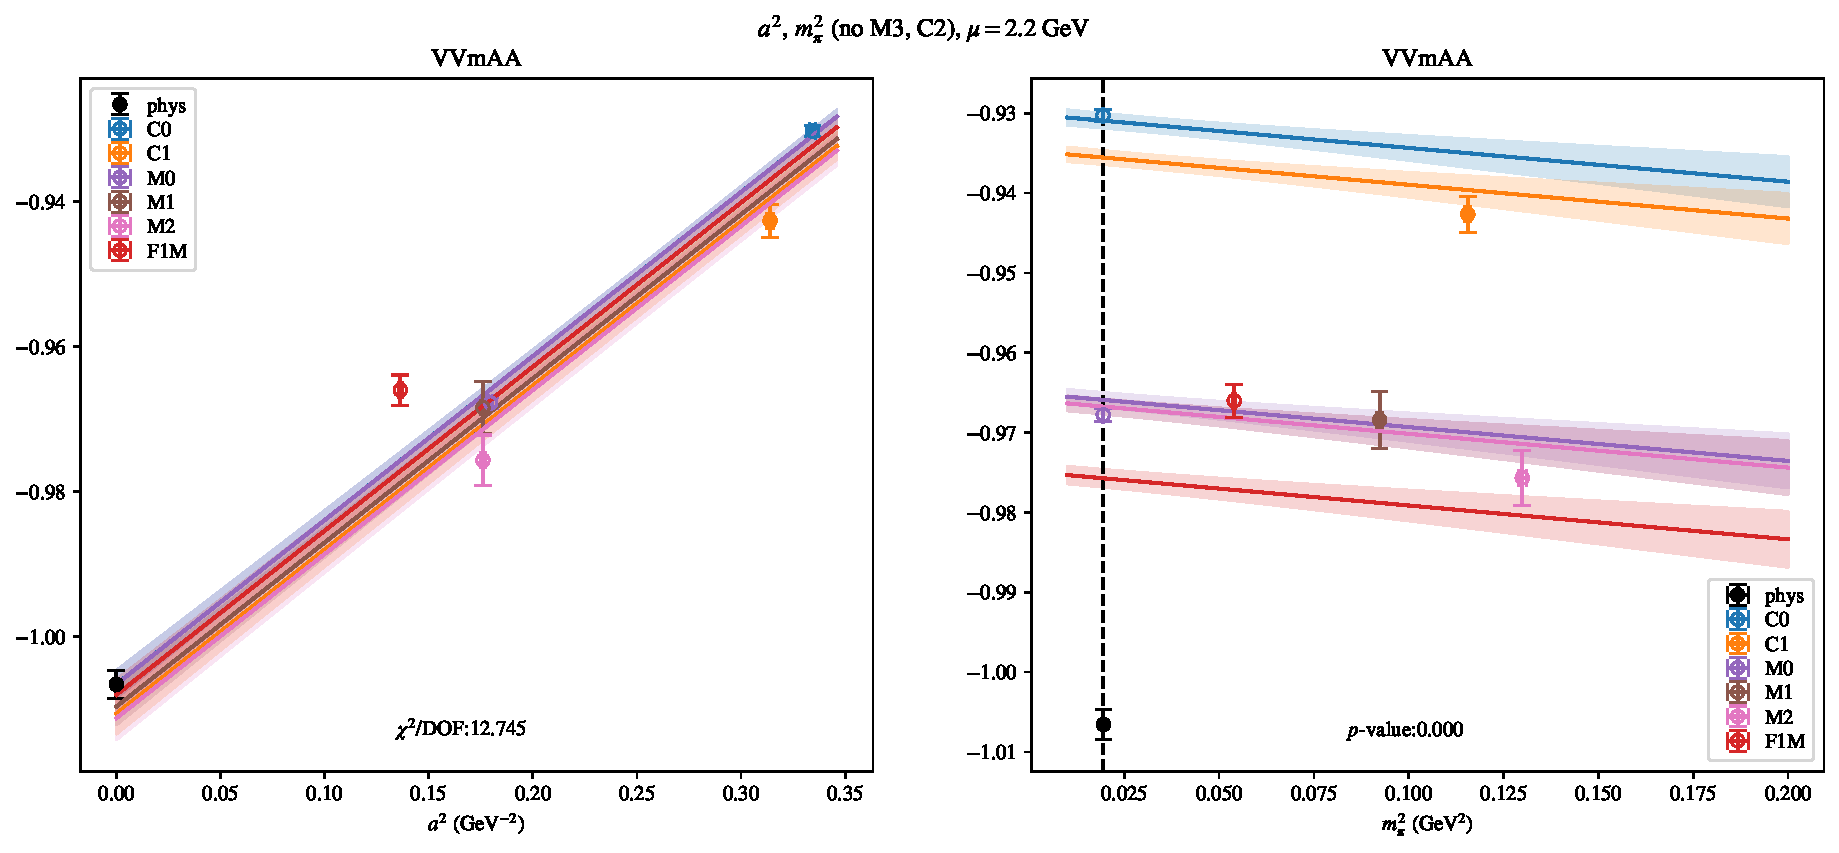
\includepdf[link, pages=-]{VVmAA/NPR/bag_a2m2mcut_22.pdf}
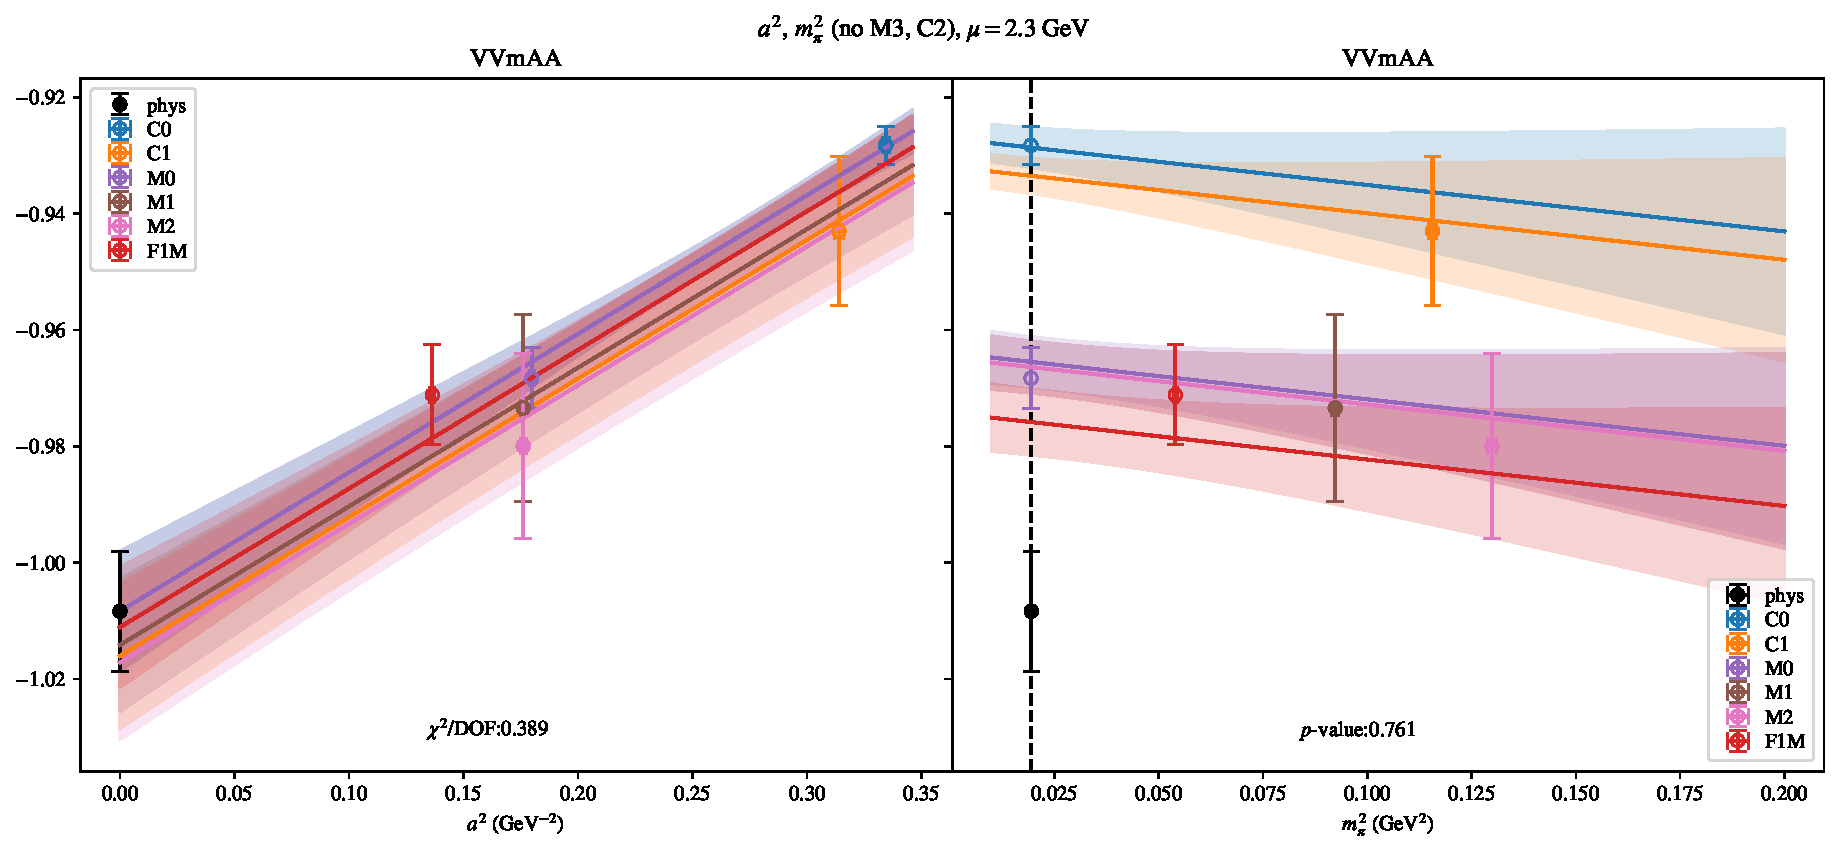
\includepdf[link, pages=-]{VVmAA/NPR/bag_a2m2mcut_23.pdf}
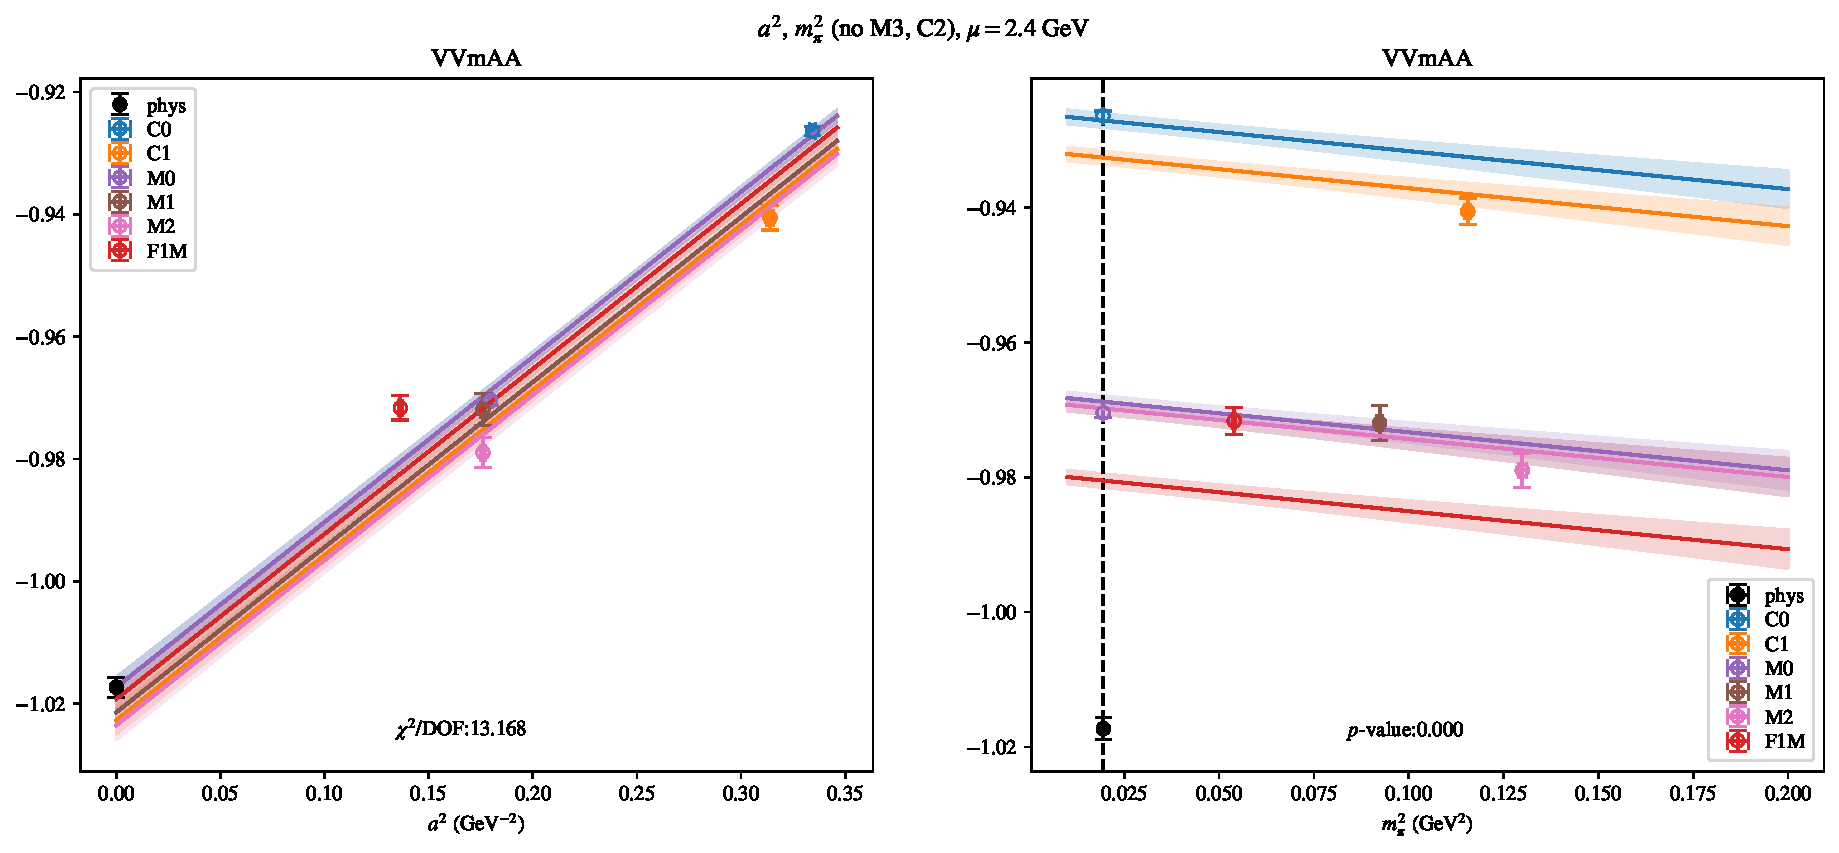
\includepdf[link, pages=-]{VVmAA/NPR/bag_a2m2mcut_24.pdf}
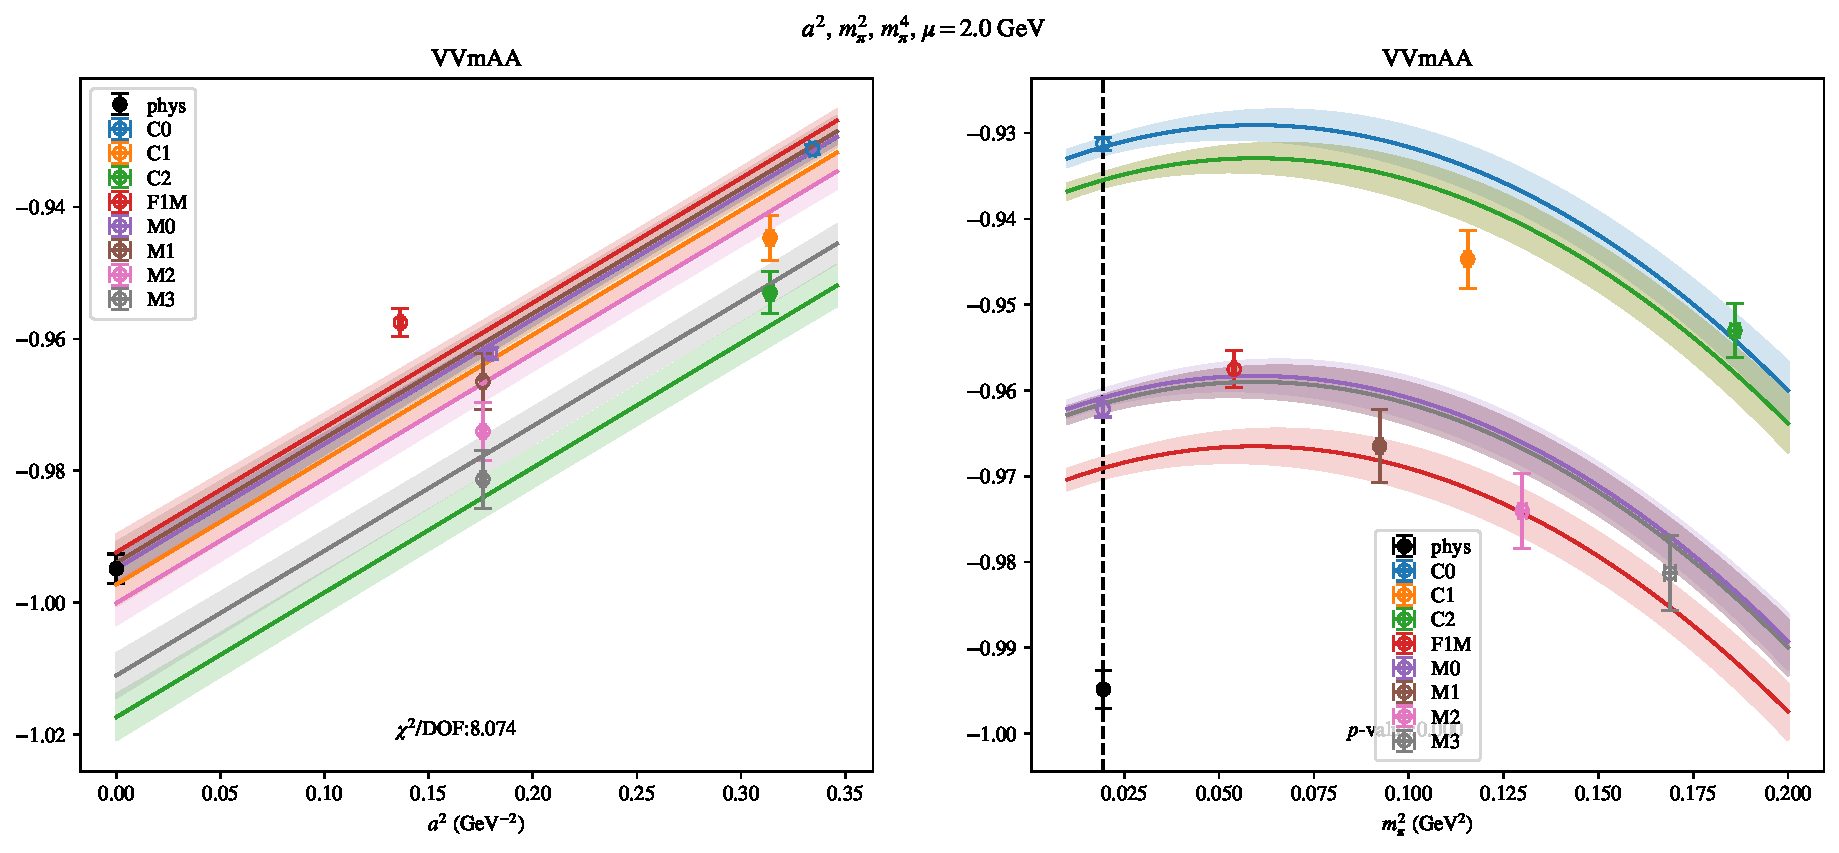
\includepdf[link, pages=-]{VVmAA/NPR/bag_a2m2m4_20.pdf}
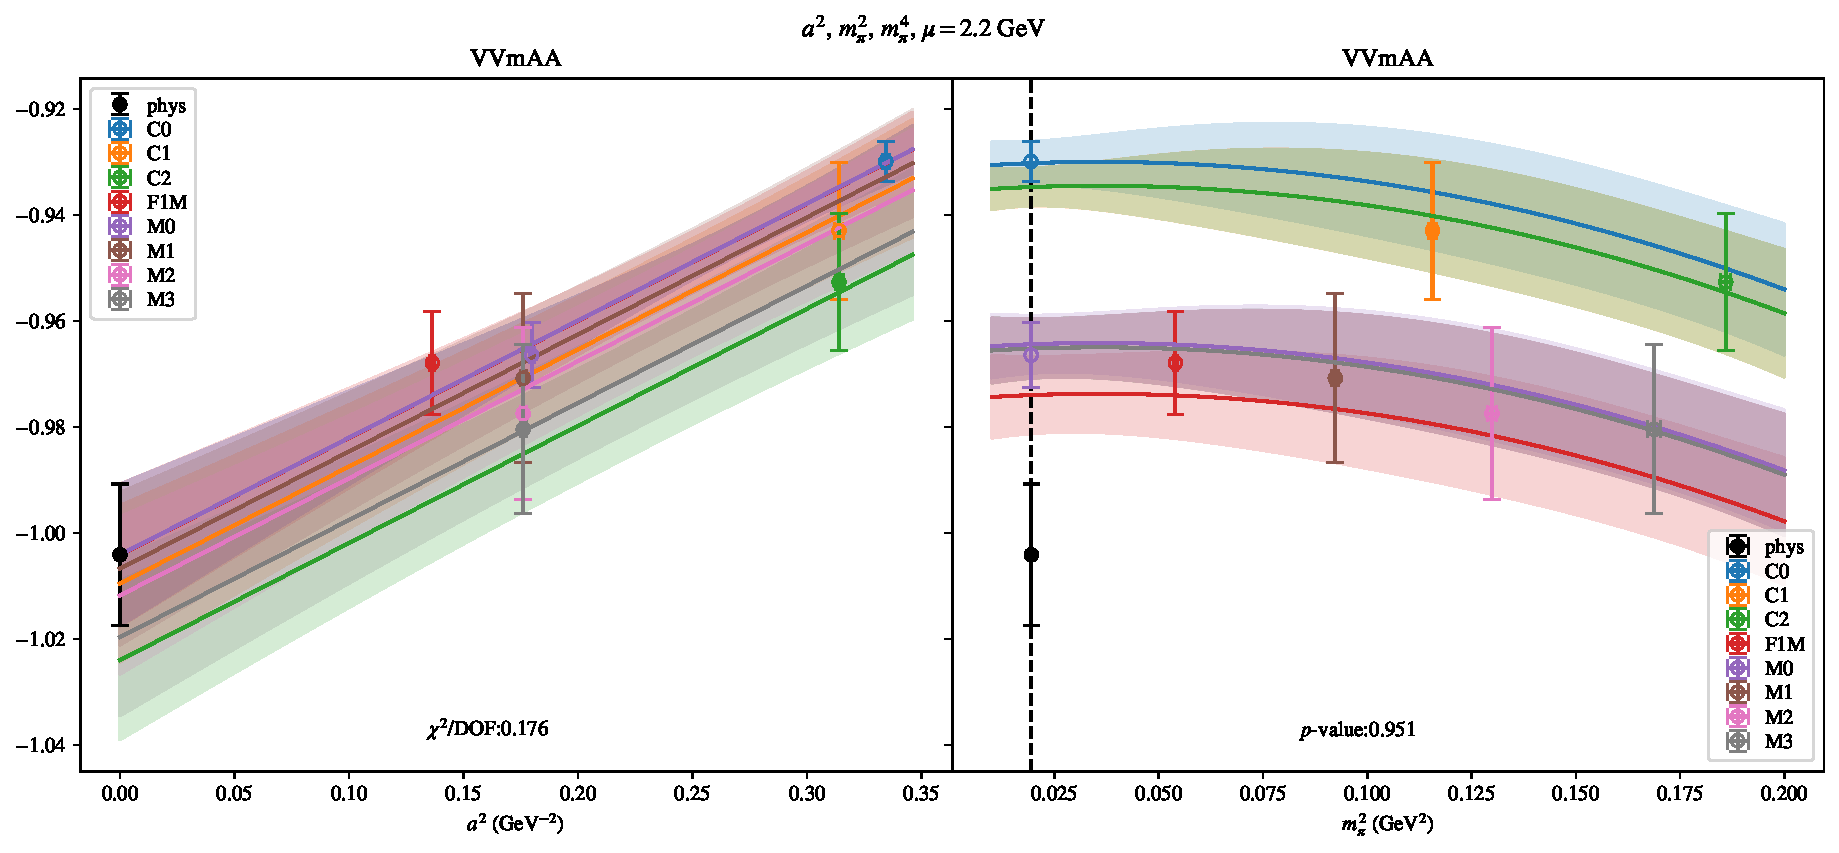
\includepdf[link, pages=-]{VVmAA/NPR/bag_a2m2m4_22.pdf}
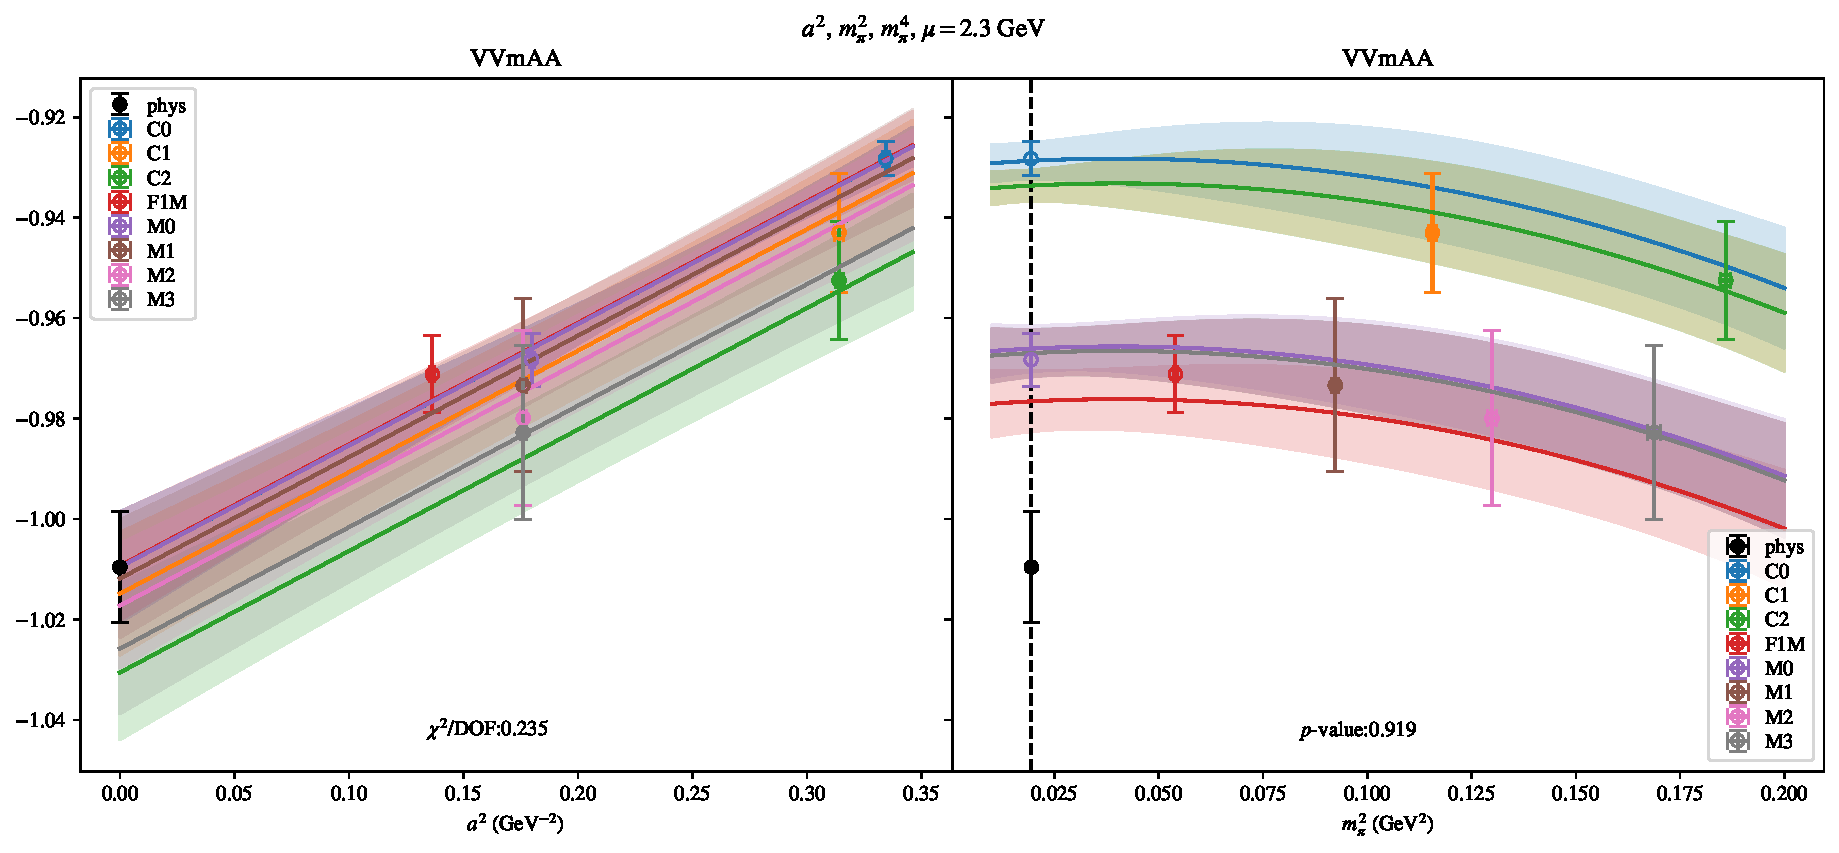
\includepdf[link, pages=-]{VVmAA/NPR/bag_a2m2m4_23.pdf}
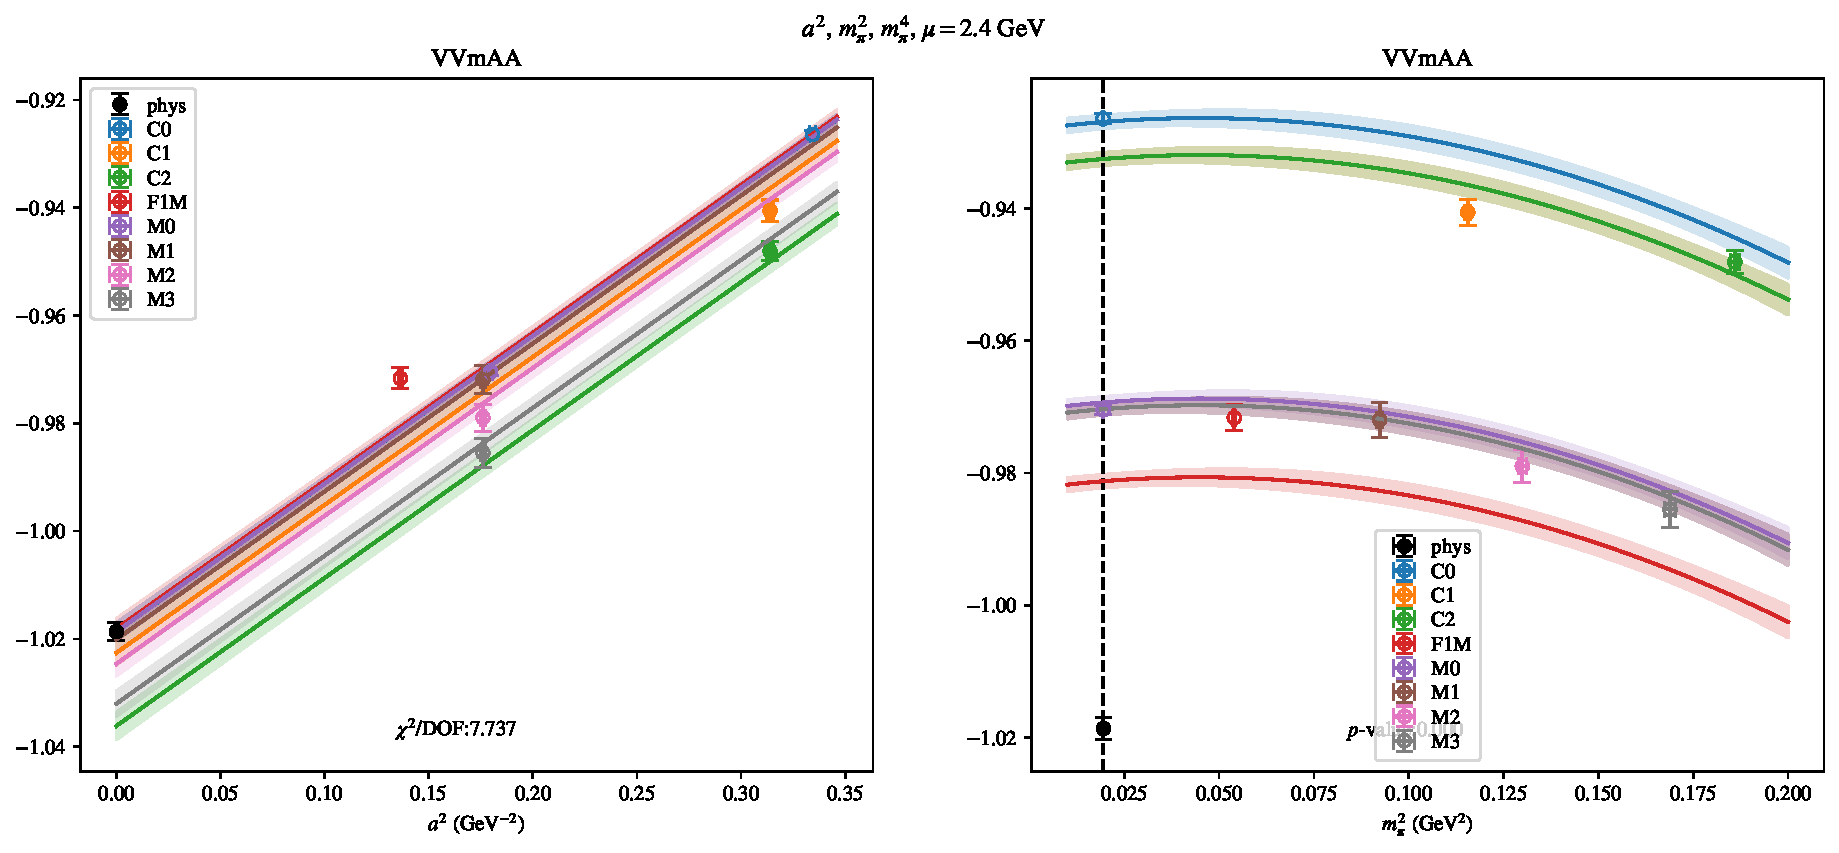
\includepdf[link, pages=-]{VVmAA/NPR/bag_a2m2m4_24.pdf}
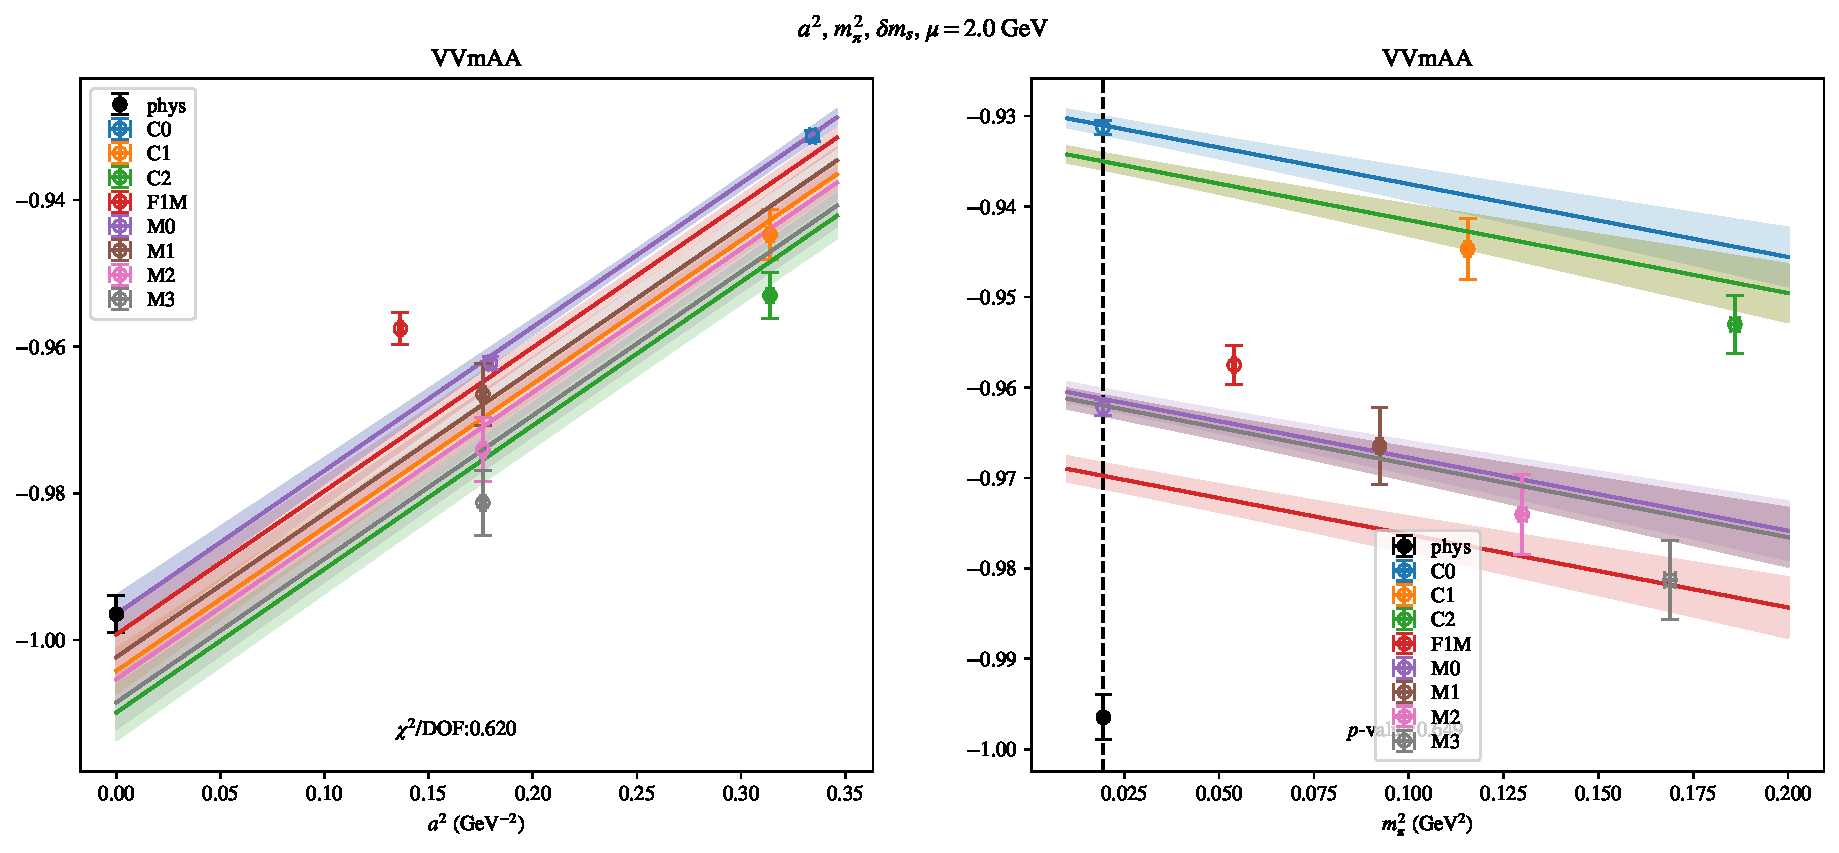
\includepdf[link, pages=-]{VVmAA/NPR/bag_a2m2delm_20.pdf}
\includepdf[link, pages=-]{VVmAA/NPR/bag_a2m2delm_22.pdf}
\includepdf[link, pages=-]{VVmAA/NPR/bag_a2m2delm_23.pdf}
\includepdf[link, pages=-]{VVmAA/NPR/bag_a2m2delm_24.pdf}
\clearpage
\section{$\mathcal{B}_3$}
\begin{table}[h!]
\begin{center}
\begin{tabular}{|c|c|c|c|c|c|c|}
\hline
$\mu$ (GeV) & $a^2$, $m_\pi^2$& $a^2$, $m_\pi^2$ (no C)& $a^2$, $m_\pi^2$, $a^4$& $a^2$, $m_\pi^2$ (no M3, C2)& $a^2$, $m_\pi^2$, $m_\pi^4$& $a^2$, $m_\pi^2$, $\delta m_s$\\
\hline
2.0& \hyperlink{SSmPP/NPR/bag_a2m2_20.pdf.1}{\textbf{1.7945(30)}: 9.735 (0.0)} & \hyperlink{SSmPP/NPR/bag_a2m2noC_20.pdf.1}{\textbf{1.706(13)}: 0.231 (0.794)} & \hyperlink{SSmPP/NPR/bag_a2a4m2_20.pdf.1}{\textbf{1.647(22)}: 0.867 (0.483)} & \hyperlink{SSmPP/NPR/bag_a2m2mcut_20.pdf.1}{\textbf{1.7939(34)}: 17.355 (0.0)} & \hyperlink{SSmPP/NPR/bag_a2m2m4_20.pdf.1}{\textbf{1.7983(36)}: 10.384 (0.0)} & \hyperlink{SSmPP/NPR/bag_a2m2delm_20.pdf.1}{\textbf{1.7934(36)}: 5.47 (0.0)}\\
2.2& \hyperlink{SSmPP/NPR/bag_a2m2_22.pdf.1}{\textbf{1.7994(28)}: 8.86 (0.0)} & \hyperlink{SSmPP/NPR/bag_a2m2noC_22.pdf.1}{\textbf{1.720(12)}: 0.169 (0.845)} & \hyperlink{SSmPP/NPR/bag_a2a4m2_22.pdf.1}{\textbf{1.664(21)}: 0.978 (0.418)} & \hyperlink{SSmPP/NPR/bag_a2m2mcut_22.pdf.1}{\textbf{1.8008(32)}: 14.387 (0.0)} & \hyperlink{SSmPP/NPR/bag_a2m2m4_22.pdf.1}{\textbf{1.8038(34)}: 8.738 (0.0)} & \hyperlink{SSmPP/NPR/bag_a2m2delm_22.pdf.1}{\textbf{1.7990(32)}: 6.417 (0.0)}\\
2.3& \hyperlink{SSmPP/NPR/bag_a2m2_23.pdf.1}{\textbf{1.8019(27)}: 8.332 (0.0)} & \hyperlink{SSmPP/NPR/bag_a2m2noC_23.pdf.1}{\textbf{1.725(12)}: 0.209 (0.811)} & \hyperlink{SSmPP/NPR/bag_a2a4m2_23.pdf.1}{\textbf{1.671(21)}: 0.784 (0.535)} & \hyperlink{SSmPP/NPR/bag_a2m2mcut_23.pdf.1}{\textbf{1.8030(32)}: 13.509 (0.0)} & \hyperlink{SSmPP/NPR/bag_a2m2m4_23.pdf.1}{\textbf{1.8059(34)}: 8.663 (0.0)} & \hyperlink{SSmPP/NPR/bag_a2m2delm_23.pdf.1}{\textbf{1.8015(30)}: 5.717 (0.0)}\\
2.4& \hyperlink{SSmPP/NPR/bag_a2m2_24.pdf.1}{\textbf{1.8035(28)}: 7.761 (0.0)} & \hyperlink{SSmPP/NPR/bag_a2m2noC_24.pdf.1}{\textbf{1.730(12)}: 0.187 (0.829)} & \hyperlink{SSmPP/NPR/bag_a2a4m2_24.pdf.1}{\textbf{1.678(21)}: 0.732 (0.57)} & \hyperlink{SSmPP/NPR/bag_a2m2mcut_24.pdf.1}{\textbf{1.8048(33)}: 12.436 (0.0)} & \hyperlink{SSmPP/NPR/bag_a2m2m4_24.pdf.1}{\textbf{1.8074(34)}: 8.054 (0.0)} & \hyperlink{SSmPP/NPR/bag_a2m2delm_24.pdf.1}{\textbf{1.8031(29)}: 5.07 (0.0)}\\
\hline
\end{tabular}
\caption{Physical point value from chiral and continuum extrapolation at renormalisation scale $\mu$. Entries are \textbf{value(error)}: $\chi^2/\text{DOF}$ ($p$-value).}
\end{center}
\end{table}
\begin{table}[h!]
\begin{center}
\begin{tabular}{|c c|c|c|c|c|c|c|}
\hline
$\mu$ (GeV) &  & $a^2$, $m_\pi^2$& $a^2$, $m_\pi^2$ (no C)& $a^2$, $m_\pi^2$, $a^4$& $a^2$, $m_\pi^2$ (no M3, C2)& $a^2$, $m_\pi^2$, $m_\pi^4$& $a^2$, $m_\pi^2$, $\delta m_s$\\
\hline
\multirow{3}{0.5in}{2.0} & $\alpha$ & 0.140(11)& 0.668(77)& 1.49(20)& 0.142(12)& 0.129(12)& 0.136(12)\\
 & $\beta$ & -0.00151(24)& -0.00172(50)& -0.00215(27)& -0.00187(44)& -0.0050(13)& -0.00419(56)\\
 & $\gamma$ &  &  & -2.74(40)&  & 0.00032(12)& 0.106(20)\\
\hline
\multirow{3}{0.5in}{2.2} & $\alpha$ & 0.153(10)& 0.632(74)& 1.40(19)& 0.149(12)& 0.139(12)& 0.147(11)\\
 & $\beta$ & -0.00095(22)& -0.00134(47)& -0.00157(25)& -0.00147(39)& -0.0047(12)& -0.00300(52)\\
 & $\gamma$ &  &  & -2.53(39)&  & 0.00034(10)& 0.082(18)\\
\hline
\multirow{3}{0.5in}{2.3} & $\alpha$ & 0.154(10)& 0.617(75)& 1.36(19)& 0.151(12)& 0.142(12)& 0.149(10)\\
 & $\beta$ & -0.00085(21)& -0.00124(45)& -0.00146(24)& -0.00125(40)& -0.0041(11)& -0.00285(53)\\
 & $\gamma$ &  &  & -2.44(39)&  & 0.00030(10)& 0.079(18)\\
\hline
\multirow{3}{0.5in}{2.4} & $\alpha$ & 0.157(10)& 0.603(74)& 1.32(19)& 0.153(12)& 0.145(12)& 0.152(10)\\
 & $\beta$ & -0.00077(21)& -0.00113(46)& -0.00136(24)& -0.00113(39)& -0.0037(11)& -0.00275(53)\\
 & $\gamma$ &  &  & -2.35(39)&  & 0.00026(10)& 0.079(18)\\
\hline
\end{tabular}
\caption{Fit values of coefficients in $Q = Q_{phys} + \mathbf{\alpha} a^2 + \mathbf{\beta}\left(\frac{m_\pi^2}{f_\pi^2}-\frac{m_{\pi,PDG}^2}{f_\pi^2}\right) + \gamma(\ldots)$}
\end{center}
\end{table}
\includepdf[link, pages=-]{SSmPP/NPR/bag_a2m2_20.pdf}
\includepdf[link, pages=-]{SSmPP/NPR/bag_a2m2_22.pdf}
\includepdf[link, pages=-]{SSmPP/NPR/bag_a2m2_23.pdf}
\includepdf[link, pages=-]{SSmPP/NPR/bag_a2m2_24.pdf}
\includepdf[link, pages=-]{SSmPP/NPR/bag_a2m2noC_20.pdf}
\includepdf[link, pages=-]{SSmPP/NPR/bag_a2m2noC_22.pdf}
\includepdf[link, pages=-]{SSmPP/NPR/bag_a2m2noC_23.pdf}
\includepdf[link, pages=-]{SSmPP/NPR/bag_a2m2noC_24.pdf}
\includepdf[link, pages=-]{SSmPP/NPR/bag_a2a4m2_20.pdf}
\includepdf[link, pages=-]{SSmPP/NPR/bag_a2a4m2_22.pdf}
\includepdf[link, pages=-]{SSmPP/NPR/bag_a2a4m2_23.pdf}
\includepdf[link, pages=-]{SSmPP/NPR/bag_a2a4m2_24.pdf}
\includepdf[link, pages=-]{SSmPP/NPR/bag_a2m2mcut_20.pdf}
\includepdf[link, pages=-]{SSmPP/NPR/bag_a2m2mcut_22.pdf}
\includepdf[link, pages=-]{SSmPP/NPR/bag_a2m2mcut_23.pdf}
\includepdf[link, pages=-]{SSmPP/NPR/bag_a2m2mcut_24.pdf}
\includepdf[link, pages=-]{SSmPP/NPR/bag_a2m2m4_20.pdf}
\includepdf[link, pages=-]{SSmPP/NPR/bag_a2m2m4_22.pdf}
\includepdf[link, pages=-]{SSmPP/NPR/bag_a2m2m4_23.pdf}
\includepdf[link, pages=-]{SSmPP/NPR/bag_a2m2m4_24.pdf}
\includepdf[link, pages=-]{SSmPP/NPR/bag_a2m2delm_20.pdf}
\includepdf[link, pages=-]{SSmPP/NPR/bag_a2m2delm_22.pdf}
\includepdf[link, pages=-]{SSmPP/NPR/bag_a2m2delm_23.pdf}
\includepdf[link, pages=-]{SSmPP/NPR/bag_a2m2delm_24.pdf}
\clearpage
\section{$\mathcal{B}_4$}
\begin{table}[h!]
\begin{center}
\begin{tabular}{|c|c|c|c|c|c|c|}
\hline
$\mu$ (GeV) & $a^2$, $m_\pi^2$& $a^2$, $m_\pi^2$ (no C)& $a^2$, $m_\pi^2$, $a^4$& $a^2$, $m_\pi^2$ (no M3, C2)& $a^2$, $m_\pi^2$, $m_\pi^4$& $a^2$, $m_\pi^2$, $\delta m_s$\\
\hline
2.0& \hyperlink{SSpPP/NPR/bag_a2m2_20.pdf.1}{\textbf{-0.9261(18)}: 3.582 (0.003)} & \hyperlink{SSpPP/NPR/bag_a2m2noC_20.pdf.1}{\textbf{-0.9463(80)}: 2.283 (0.102)} & \hyperlink{SSpPP/NPR/bag_a2a4m2_20.pdf.1}{\textbf{-0.947(14)}: 3.868 (0.004)} & \hyperlink{SSpPP/NPR/bag_a2m2mcut_20.pdf.1}{\textbf{-0.9253(18)}: 3.699 (0.011)} & \hyperlink{SSpPP/NPR/bag_a2m2m4_20.pdf.1}{\textbf{-0.9233(20)}: 2.372 (0.05)} & \hyperlink{SSpPP/NPR/bag_a2m2delm_20.pdf.1}{\textbf{-0.9260(18)}: 4.391 (0.002)}\\
2.2& \hyperlink{SSpPP/NPR/bag_a2m2_22.pdf.1}{\textbf{-0.9061(17)}: 4.545 (0.0)} & \hyperlink{SSpPP/NPR/bag_a2m2noC_22.pdf.1}{\textbf{-0.9299(72)}: 1.673 (0.188)} & \hyperlink{SSpPP/NPR/bag_a2a4m2_22.pdf.1}{\textbf{-0.930(13)}: 5.027 (0.0)} & \hyperlink{SSpPP/NPR/bag_a2m2mcut_22.pdf.1}{\textbf{-0.9061(18)}: 4.641 (0.003)} & \hyperlink{SSpPP/NPR/bag_a2m2m4_22.pdf.1}{\textbf{-0.9039(19)}: 4.171 (0.002)} & \hyperlink{SSpPP/NPR/bag_a2m2delm_22.pdf.1}{\textbf{-0.9064(17)}: 5.704 (0.0)}\\
2.3& \hyperlink{SSpPP/NPR/bag_a2m2_23.pdf.1}{\textbf{-0.8975(16)}: 5.412 (0.0)} & \hyperlink{SSpPP/NPR/bag_a2m2noC_23.pdf.1}{\textbf{-0.9226(72)}: 2.085 (0.124)} & \hyperlink{SSpPP/NPR/bag_a2a4m2_23.pdf.1}{\textbf{-0.922(13)}: 5.849 (0.0)} & \hyperlink{SSpPP/NPR/bag_a2m2mcut_23.pdf.1}{\textbf{-0.8973(17)}: 5.81 (0.001)} & \hyperlink{SSpPP/NPR/bag_a2m2m4_23.pdf.1}{\textbf{-0.8952(17)}: 4.511 (0.001)} & \hyperlink{SSpPP/NPR/bag_a2m2delm_23.pdf.1}{\textbf{-0.8978(17)}: 6.558 (0.0)}\\
2.4& \hyperlink{SSpPP/NPR/bag_a2m2_24.pdf.1}{\textbf{-0.8901(16)}: 5.729 (0.0)} & \hyperlink{SSpPP/NPR/bag_a2m2noC_24.pdf.1}{\textbf{-0.9154(76)}: 2.068 (0.126)} & \hyperlink{SSpPP/NPR/bag_a2a4m2_24.pdf.1}{\textbf{-0.915(12)}: 6.145 (0.0)} & \hyperlink{SSpPP/NPR/bag_a2m2mcut_24.pdf.1}{\textbf{-0.8896(17)}: 7.045 (0.0)} & \hyperlink{SSpPP/NPR/bag_a2m2m4_24.pdf.1}{\textbf{-0.8871(18)}: 4.833 (0.001)} & \hyperlink{SSpPP/NPR/bag_a2m2delm_24.pdf.1}{\textbf{-0.8898(16)}: 7.09 (0.0)}\\
\hline
\end{tabular}
\caption{Physical point value from chiral and continuum extrapolation at renormalisation scale $\mu$. Entries are \textbf{value(error)}: $\chi^2/\text{DOF}$ ($p$-value).}
\end{center}
\end{table}
\begin{table}[h!]
\begin{center}
\begin{tabular}{|c c|c|c|c|c|c|c|}
\hline
$\mu$ (GeV) &  & $a^2$, $m_\pi^2$& $a^2$, $m_\pi^2$ (no C)& $a^2$, $m_\pi^2$, $a^4$& $a^2$, $m_\pi^2$ (no M3, C2)& $a^2$, $m_\pi^2$, $m_\pi^4$& $a^2$, $m_\pi^2$, $\delta m_s$\\
\hline
\multirow{3}{0.5in}{2.0} & $\alpha$ & -0.3481(69)& -0.232(46)& -0.16(12)& -0.3503(69)& -0.3571(72)& -0.3487(72)\\
 & $\beta$ & -0.00626(15)& -0.00586(26)& -0.00635(15)& -0.00674(25)& -0.00860(79)& -0.00629(36)\\
 & $\gamma$ &  &  & -0.39(26)&  & 0.000213(70)& 0.0007(141)\\
\hline
\multirow{3}{0.5in}{2.2} & $\alpha$ & -0.3837(66)& -0.249(41)& -0.17(12)& -0.3828(67)& -0.3905(69)& -0.3830(70)\\
 & $\beta$ & -0.00650(14)& -0.00596(27)& -0.00659(14)& -0.00693(26)& -0.00850(75)& -0.00656(34)\\
 & $\gamma$ &  &  & -0.43(24)&  & 0.000183(67)& 0.002(13)\\
\hline
\multirow{3}{0.5in}{2.3} & $\alpha$ & -0.3990(64)& -0.257(42)& -0.18(12)& -0.3988(67)& -0.4061(64)& -0.3983(70)\\
 & $\beta$ & -0.00653(13)& -0.00600(24)& -0.00664(14)& -0.00698(25)& -0.00877(71)& -0.00658(34)\\
 & $\gamma$ &  &  & -0.45(24)&  & 0.000204(62)& 0.003(13)\\
\hline
\multirow{3}{0.5in}{2.4} & $\alpha$ & -0.4115(63)& -0.267(44)& -0.18(11)& -0.4124(66)& -0.4208(65)& -0.4129(66)\\
 & $\beta$ & -0.00654(14)& -0.00601(25)& -0.00665(13)& -0.00689(24)& -0.00879(73)& -0.00661(34)\\
 & $\gamma$ &  &  & -0.47(24)&  & 0.000204(65)& 0.002(14)\\
\hline
\end{tabular}
\caption{Fit values of coefficients in $Q = Q_{phys} + \mathbf{\alpha} a^2 + \mathbf{\beta}\left(\frac{m_\pi^2}{f_\pi^2}-\frac{m_{\pi,PDG}^2}{f_\pi^2}\right) + \gamma(\ldots)$}
\end{center}
\end{table}
\includepdf[link, pages=-]{SSpPP/NPR/bag_a2m2_20.pdf}
\includepdf[link, pages=-]{SSpPP/NPR/bag_a2m2_22.pdf}
\includepdf[link, pages=-]{SSpPP/NPR/bag_a2m2_23.pdf}
\includepdf[link, pages=-]{SSpPP/NPR/bag_a2m2_24.pdf}
\includepdf[link, pages=-]{SSpPP/NPR/bag_a2m2noC_20.pdf}
\includepdf[link, pages=-]{SSpPP/NPR/bag_a2m2noC_22.pdf}
\includepdf[link, pages=-]{SSpPP/NPR/bag_a2m2noC_23.pdf}
\includepdf[link, pages=-]{SSpPP/NPR/bag_a2m2noC_24.pdf}
\includepdf[link, pages=-]{SSpPP/NPR/bag_a2a4m2_20.pdf}
\includepdf[link, pages=-]{SSpPP/NPR/bag_a2a4m2_22.pdf}
\includepdf[link, pages=-]{SSpPP/NPR/bag_a2a4m2_23.pdf}
\includepdf[link, pages=-]{SSpPP/NPR/bag_a2a4m2_24.pdf}
\includepdf[link, pages=-]{SSpPP/NPR/bag_a2m2mcut_20.pdf}
\includepdf[link, pages=-]{SSpPP/NPR/bag_a2m2mcut_22.pdf}
\includepdf[link, pages=-]{SSpPP/NPR/bag_a2m2mcut_23.pdf}
\includepdf[link, pages=-]{SSpPP/NPR/bag_a2m2mcut_24.pdf}
\includepdf[link, pages=-]{SSpPP/NPR/bag_a2m2m4_20.pdf}
\includepdf[link, pages=-]{SSpPP/NPR/bag_a2m2m4_22.pdf}
\includepdf[link, pages=-]{SSpPP/NPR/bag_a2m2m4_23.pdf}
\includepdf[link, pages=-]{SSpPP/NPR/bag_a2m2m4_24.pdf}
\includepdf[link, pages=-]{SSpPP/NPR/bag_a2m2delm_20.pdf}
\includepdf[link, pages=-]{SSpPP/NPR/bag_a2m2delm_22.pdf}
\includepdf[link, pages=-]{SSpPP/NPR/bag_a2m2delm_23.pdf}
\includepdf[link, pages=-]{SSpPP/NPR/bag_a2m2delm_24.pdf}
\clearpage
\section{$\mathcal{B}_5$}
\begin{table}[h!]
\begin{center}
\begin{tabular}{|c|c|c|c|c|c|c|}
\hline
$\mu$ (GeV) & $a^2$, $m_\pi^2$& $a^2$, $m_\pi^2$ (no C)& $a^2$, $m_\pi^2$, $a^4$& $a^2$, $m_\pi^2$ (no M3, C2)& $a^2$, $m_\pi^2$, $m_\pi^4$& $a^2$, $m_\pi^2$, $\delta m_s$\\
\hline
2.0& \hyperlink{TT/NPR/bag_a2m2_20.pdf.1}{\textbf{-0.3621(43)}: 0.053 (0.998)} & \hyperlink{TT/NPR/bag_a2m2noC_20.pdf.1}{\textbf{-0.369(20)}: 0.024 (0.977)} & \hyperlink{TT/NPR/bag_a2a4m2_20.pdf.1}{\textbf{-0.370(30)}: 0.058 (0.994)} & \hyperlink{TT/NPR/bag_a2m2mcut_20.pdf.1}{\textbf{-0.3623(48)}: 0.043 (0.988)} & \hyperlink{TT/NPR/bag_a2m2m4_20.pdf.1}{\textbf{-0.3616(51)}: 0.033 (0.998)} & \hyperlink{TT/NPR/bag_a2m2delm_20.pdf.1}{\textbf{-0.3625(43)}: 0.071 (0.991)}\\
2.2& \hyperlink{TT/NPR/bag_a2m2_22.pdf.1}{\textbf{-0.3597(36)}: 0.076 (0.996)} & \hyperlink{TT/NPR/bag_a2m2noC_22.pdf.1}{\textbf{-0.367(17)}: 0.015 (0.985)} & \hyperlink{TT/NPR/bag_a2a4m2_22.pdf.1}{\textbf{-0.367(27)}: 0.077 (0.989)} & \hyperlink{TT/NPR/bag_a2m2mcut_22.pdf.1}{\textbf{-0.3596(42)}: 0.082 (0.97)} & \hyperlink{TT/NPR/bag_a2m2m4_22.pdf.1}{\textbf{-0.3591(43)}: 0.064 (0.992)} & \hyperlink{TT/NPR/bag_a2m2delm_22.pdf.1}{\textbf{-0.3597(38)}: 0.095 (0.984)}\\
2.3& \hyperlink{TT/NPR/bag_a2m2_23.pdf.1}{\textbf{-0.3588(31)}: 0.099 (0.992)} & \hyperlink{TT/NPR/bag_a2m2noC_23.pdf.1}{\textbf{-0.366(15)}: 0.026 (0.974)} & \hyperlink{TT/NPR/bag_a2a4m2_23.pdf.1}{\textbf{-0.365(27)}: 0.112 (0.978)} & \hyperlink{TT/NPR/bag_a2m2mcut_23.pdf.1}{\textbf{-0.3585(37)}: 0.087 (0.967)} & \hyperlink{TT/NPR/bag_a2m2m4_23.pdf.1}{\textbf{-0.3580(36)}: 0.068 (0.992)} & \hyperlink{TT/NPR/bag_a2m2delm_23.pdf.1}{\textbf{-0.3586(33)}: 0.123 (0.974)}\\
2.4& \hyperlink{TT/NPR/bag_a2m2_24.pdf.1}{\textbf{-0.3579(32)}: 0.123 (0.987)} & \hyperlink{TT/NPR/bag_a2m2noC_24.pdf.1}{\textbf{-0.365(14)}: 0.043 (0.958)} & \hyperlink{TT/NPR/bag_a2a4m2_24.pdf.1}{\textbf{-0.364(24)}: 0.142 (0.967)} & \hyperlink{TT/NPR/bag_a2m2mcut_24.pdf.1}{\textbf{-0.3575(36)}: 0.107 (0.956)} & \hyperlink{TT/NPR/bag_a2m2m4_24.pdf.1}{\textbf{-0.3571(35)}: 0.065 (0.992)} & \hyperlink{TT/NPR/bag_a2m2delm_24.pdf.1}{\textbf{-0.3579(30)}: 0.151 (0.963)}\\
\hline
\end{tabular}
\caption{Physical point value from chiral and continuum extrapolation at renormalisation scale $\mu$. Entries are \textbf{value(error)}: $\chi^2/\text{DOF}$ ($p$-value).}
\end{center}
\end{table}
\begin{table}[h!]
\begin{center}
\begin{tabular}{|c c|c|c|c|c|c|c|}
\hline
$\mu$ (GeV) &  & $a^2$, $m_\pi^2$& $a^2$, $m_\pi^2$ (no C)& $a^2$, $m_\pi^2$, $a^4$& $a^2$, $m_\pi^2$ (no M3, C2)& $a^2$, $m_\pi^2$, $m_\pi^4$& $a^2$, $m_\pi^2$, $\delta m_s$\\
\hline
\multirow{3}{0.5in}{2.0} & $\alpha$ & 0.012(15)& 0.05(12)& 0.08(28)& 0.013(16)& 0.010(17)& 0.013(15)\\
 & $\beta$ & -0.00223(25)& -0.00218(61)& -0.00227(30)& -0.00235(48)& -0.0028(14)& -0.00221(57)\\
 & $\gamma$ &  &  & -0.14(57)&  & 0.00005(11)& -0.001(20)\\
\hline
\multirow{3}{0.5in}{2.2} & $\alpha$ & 0.028(12)& 0.07(10)& 0.10(24)& 0.028(14)& 0.026(14)& 0.028(13)\\
 & $\beta$ & -0.00229(23)& -0.00220(47)& -0.00233(30)& -0.00238(38)& -0.0027(11)& -0.00229(55)\\
 & $\gamma$ &  &  & -0.15(50)&  & 0.000036(98)& 0.00002(1891)\\
\hline
\multirow{3}{0.5in}{2.3} & $\alpha$ & 0.037(11)& 0.077(92)& 0.10(25)& 0.036(13)& 0.035(12)& 0.036(12)\\
 & $\beta$ & -0.00228(22)& -0.00221(42)& -0.00231(27)& -0.00241(38)& -0.0028(10)& -0.00223(55)\\
 & $\gamma$ &  &  & -0.12(52)&  & 0.000047(90)& -0.002(18)\\
\hline
\multirow{3}{0.5in}{2.4} & $\alpha$ & 0.045(11)& 0.085(83)& 0.10(22)& 0.045(12)& 0.043(11)& 0.046(10)\\
 & $\beta$ & -0.00225(21)& -0.00221(43)& -0.00228(23)& -0.00239(35)& -0.0028(10)& -0.00218(46)\\
 & $\gamma$ &  &  & -0.12(45)&  & 0.000052(90)& -0.003(16)\\
\hline
\end{tabular}
\caption{Fit values of coefficients in $Q = Q_{phys} + \mathbf{\alpha} a^2 + \mathbf{\beta}\left(\frac{m_\pi^2}{f_\pi^2}-\frac{m_{\pi,PDG}^2}{f_\pi^2}\right) + \gamma(\ldots)$}
\end{center}
\end{table}
\includepdf[link, pages=-]{TT/NPR/bag_a2m2_20.pdf}
\includepdf[link, pages=-]{TT/NPR/bag_a2m2_22.pdf}
\includepdf[link, pages=-]{TT/NPR/bag_a2m2_23.pdf}
\includepdf[link, pages=-]{TT/NPR/bag_a2m2_24.pdf}
\includepdf[link, pages=-]{TT/NPR/bag_a2m2noC_20.pdf}
\includepdf[link, pages=-]{TT/NPR/bag_a2m2noC_22.pdf}
\includepdf[link, pages=-]{TT/NPR/bag_a2m2noC_23.pdf}
\includepdf[link, pages=-]{TT/NPR/bag_a2m2noC_24.pdf}
\includepdf[link, pages=-]{TT/NPR/bag_a2a4m2_20.pdf}
\includepdf[link, pages=-]{TT/NPR/bag_a2a4m2_22.pdf}
\includepdf[link, pages=-]{TT/NPR/bag_a2a4m2_23.pdf}
\includepdf[link, pages=-]{TT/NPR/bag_a2a4m2_24.pdf}
\includepdf[link, pages=-]{TT/NPR/bag_a2m2mcut_20.pdf}
\includepdf[link, pages=-]{TT/NPR/bag_a2m2mcut_22.pdf}
\includepdf[link, pages=-]{TT/NPR/bag_a2m2mcut_23.pdf}
\includepdf[link, pages=-]{TT/NPR/bag_a2m2mcut_24.pdf}
\includepdf[link, pages=-]{TT/NPR/bag_a2m2m4_20.pdf}
\includepdf[link, pages=-]{TT/NPR/bag_a2m2m4_22.pdf}
\includepdf[link, pages=-]{TT/NPR/bag_a2m2m4_23.pdf}
\includepdf[link, pages=-]{TT/NPR/bag_a2m2m4_24.pdf}
\includepdf[link, pages=-]{TT/NPR/bag_a2m2delm_20.pdf}
\includepdf[link, pages=-]{TT/NPR/bag_a2m2delm_22.pdf}
\includepdf[link, pages=-]{TT/NPR/bag_a2m2delm_23.pdf}
\includepdf[link, pages=-]{TT/NPR/bag_a2m2delm_24.pdf}
\clearpage
\end{document}